\documentclass[12pt]{My_preprint}
\title{
    Theoretical calculation of the droplet induced agitation (or pseudoturbulence) in mono disperse buoyant emulsions for low inertia and dilute regime.
    }

\author[1,2]{Nicolas Fintzi}
% \author[1]{Jean-Lou Pierson}
% \author[2]{Stephane Popinet}
\affil[1]{IFP Energies Nouvelles, Rond-point de l’echangeur de Solaize, 69360 Solaize}
\affil[2]{Sorbonne Universit\'e, Institut Jean le Rond d'Alembert, 4 place Jussieu, 75252 PARIS CEDEX 05, France}
\normalmarginpar


\begin{document}

\maketitle

\begin{abstract}
    In this study we derive an analytical expression for the continuous phase \textit{Reynolds stress} tensor. 
    This derivation is restricted to the dilute regime where the dispersed phase volume fraction labeled $\phi$ is vanishingly small and for particle Reynolds number $Re \ll 1$. 
    In this context we derive an analytical formula for the pseudoturbulence generated by translating bubbles or droplets inside a Newtonian fluid. 
    To by-pass the integral convergence difficulties generated due to the $\mathcal{O}(r^{-1})$ decay of the disturbance velocity field we make use of the Nearest-Particle-Statistical (NPS) as it is introduced in \citet{zhang2023evolution}. 
\end{abstract}


% 
\section{Introduction}


In this chapter, we focus on the modeling of what is called the \textit{Pseudo-turbulent} stress tensor, or \textit{Reynolds stress} tensor. 
The former terminology is more appropriate since we consider, in this chapter, the modeling of the velocity fluctuations that are generated by the motion of the particles. 
In other words, we focus on the modeling of the velocity fluctuation generated by the wakes or the disturbance velocity fields of the droplets. 

% Our first approach of modeling will be entirely theoretical.
% Then in a second step, we extend the model obtained in the previous step with we use of the results obtained with the DNS presented in the last chapters.  

The \textit{Pseudo-turbulence} stress tenor represents the averaged local values of the velocity fluctuation generated by the motion of the particles present in the flow. 
Therefore, we first need to model the disturbance field generated by a particle immersed in an arbitrary flow and then average it over the carrier fluid phase to obtain the \textit{Pseudo-turbulence} stress. 
To simplify the problem, we will initially consider only uniform relative motions between the droplets and the carrier fluid. 
Subsequently, we will explore the possibility of extending this approach to arbitrary flow fields, based on the general singularity solution of \citet{kim2013microhydrodynamics}. 

In this restricted situation the \textit{Pseudo-turbulence} stress corresponds to the velocity variance, generated due to a droplet in translation relative to a quiescent fluid.
Within this context, \citet{van1998pseudo} computed a \textit{Pseudo turbulence} stress closure model for mono-disperse bubbles rising in a quiescent fluid. 
His model is based on the potential flow solution of the wake generated by a translating bubble in stokes flows.
Then, we perform a similar analysis for a droplet translating in Stokes flow instead of potential flow. In this regime, the wake generated by the droplet decays as $\mathcal{O}(r^{-1})$ with $\textbf{r}$ is the distance from the droplet's center of mass to a point in space. 
This slow decay of the disturbance field prevents us from using the same statistical considerations as \citet{van1998pseudo}  since this approach leads to divergent integrals in the Stokes flow regime, as discussed by \citet{caflisch1985variance}. 


To address this issue, we first present the classical approach of \citet{van1998pseudo} applied to the wake of a particle in Stokes flow. 
By doing so, we demonstrate why this method fails and why the computed \textit{Pseudo-turbulence} stress results in a divergent integral. 
Next, we extend the \textit{Nearest Neighbor Statistics} framework of \citet{zhang2021ensemble} and show how the ensemble-averaged \textit{Pseudo-turbulent} stress tensor is connected to the \textit{nearest neighbor conditionally averaged} wakes of the particles. 
We then demonstrate that the \textit{nearest neighbor conditionally averaged} disturbance velocity field around a particle satisfies the \textit{nearest neighbor conditionally averaged} momentum and mass equation. 
Since these equations are unsolvable in their general form, we consider a dilute emulsion and neglect the effects of inertia.
Solving these equations allows us to compute the \textit{Pseudo-turbulent} stress tensor in the dilute and Stokes regime. 
At this stage, we obtain a closure term of the \textit{Pseudo-turbulent} stress tensor adapted for Stokes flow and dependent on the viscosity ratio, the particle phase velocity variance and the particle fluid mean drift velocity.  


After rigorously validating this model, we attempt to extend the original closure for translating droplets to account for finite $Re$ and $\phi$ based on DNS results.
This new semi-empirical model is then shown to exhibit very good agreement to both experimental and numerical studies in the literature. 

Finally, based on theoretical grounds, we extend the model's applicability by incorporating mean shearing motion from the fluid phase into the \textit{nearest neighbor conditionally averaged} momentum and mass equations. 
This results in a fully closed model that accounts for the mean gradients of the fluid phase.
% \section{Closure with one-point statistics, and why it does not work for Stokes flows.}

The classical method used to close theoretically ensemble average terms, such as the \textit{Reynolds} stress tensor, namely 
\begin{equation*}
    \avg{\chi_f \textbf{u}_f' \textbf{u}_f'}[\textbf{x},t],
\end{equation*} 
is to use conditional averaged variables.
We recall that $\avg{\ldots}$ is an ensemble average procedure and that $\textbf{u}_f' = \textbf{u}_f^0 - \textbf{u}_f$ with,  $\textbf{u}_f^0$ and $\textbf{u}_f$ being the local and averaged velocity respectively.
This is what \citet{van1998pseudo} did in order to take in account the wake generated by translating bubble in potential flows. 
Here we revisit his method and show why it doesn't work for stokes flows. 

We introduce the distribution $\delta_1[\textbf{x},\textbf{w},\FF,t]$, which is non-null at the coordinate $\textbf{y}$ and $\textbf{w}$ as soon as a particle center of mass $\textbf{x}_i$ is located at $\textbf{y}$ with a center of mass velocity $\textbf{u}_i$ equal to $\textbf{w}$, namely, 
\begin{equation*}
    \delta_1[\textbf{x},\textbf{w},\FF,t] =\sum_i^N \delta(\textbf{x}_i[\FF,t] - \textbf{y})\delta(\textbf{u}_i[\FF,t] - \textbf{w}),
\end{equation*}
where $N$ is the total number of particles in the flow. 
Using this distribution and the fact that, 
\begin{equation*}
    \int_{\mathbb{R}^6}
    \delta_1
    d \textbf{y}
    d \textbf{w}
    = 1,
\end{equation*}
we can show without any assumption that, 
\begin{align}
    \avg{\chi_f \textbf{u}_f' \textbf{u}_f'}[\textbf{x},t]
    &= \frac{1}{N}
    \int_{\mathbb{R}^6}
    \avg{\delta_1\chi_f \textbf{u}_f' \textbf{u}_f'}[\textbf{x},t]
    d\textbf{y}
    d\textbf{w}\\
    &= 
    \frac{1}{N}
    \int_{\mathbb{R}^6}
    \textbf{u}_f^{1d}
    \textbf{u}_f^{1d}
    P_{1f}
    d\textbf{y}
    d\textbf{w}
    + 
    \frac{1}{N}
    \int_{\mathbb{R}^6}
    % \textbf{u}_f^{1d}
    % \textbf{u}_f^{1d}
    \avg{\delta_1 \chi_f\textbf{u}_f'' \textbf{u}_f''}
    d\textbf{y}
    d\textbf{w}
    \label{eq:classic_avg}
\end{align}
Where we have introduced,  
\begin{align}
    P_{1f} [\textbf{w},\textbf{y},\textbf{x},t]
    % = n_p[\textbf{y},\textbf{w},t] \phi_f^1[\textbf{x},t|\textbf{y},\textbf{w}], 
    =
    \avg{\chi_f \delta_1},
    % \textbf{u}_f^{1d}P_{1f} [\textbf{w},\textbf{y},\textbf{x},t]
    % = n_p[\textbf{y},\textbf{w},t] \phi_f^1[\textbf{x},t|\textbf{y},\textbf{w}], 
    % =
    % \avg{\chi_f \delta_1\textbf{u}_f^0}
    % - P_{1f} \textbf{u}_f,
\end{align}
as the probability of having a particle with velocity \textbf{w} at \textbf{y} while the continuous phase is present at \textbf{x}.
Notice that $P_{1f}$ can be subdivided into two distribution, namely, 
\begin{equation}
    P_{1f} [\textbf{w},\textbf{y},\textbf{x},t]
    = n_p[\textbf{y},\textbf{w},t] \phi_f^1[\textbf{x},t|\textbf{y},\textbf{w}],
\end{equation}
where $n_p$ is the number density and $\phi_f^1$ the fluid phase volume fraction at $\textbf{x}$ knowing a particle is present at $\textbf{y}$. 
Notice that for identical spherical particles of radius $a$, $\phi_f^1 = 0\; \forall \;|\textbf{x}-\textbf{y}| < a$, reducing the domain of integration in \ref{eq:batchlor_avg} from $\mathbb{R}^3$ to $|\textbf{x}-\textbf{y}| > a$. 
We also defined: 
The velocity fluctuation of the local value around the ensemble average : $\textbf{u}_f' = \textbf{u}_f^0 - \textbf{u}_f$;
The fluctuation of the local velocity value around the single particle conditional average $\textbf{u}_f'' = \textbf{u}_f^0 - \textbf{u}_f^1$;
The fluctuation of the single particle conditional average around the ensemble average : $\textbf{u}_f^{1d} = \textbf{u}_f^1 - \textbf{u}_f$.
In these definitions we have used the definition, $\textbf{u}_f^1 =\avg{\chi_f \delta_1 \textbf{u}_f^1}$.  
The latter definition corresponds to the averaged distance fields generated due to the particles at $\textbf{y}$ with velocity $\textbf{w}$. 
Based on these definitions and \ref{eq:classic_avg} we state that we can separate the \textit{Reynolds stress} into two distinct contribution :  (1) the agitation generated due to the averaged wakes around the particles; (2) all other source of fluctuations such as those generated through particles interactions and the single phase turbulence. 
The second contribution of \ref{eq:classic_avg} is shown to be of $\mathcal{O}(\phi^2)$ for the wake of a translating particle in potential flows \citet[Appendix A]{zhang1994averaged}.
Therefore, we assert that this second term might always be neglected, even for stokes flows. 
Regarding the first integral of this expression, we need the explicit expression of $\textbf{u}_f^{1d}$, and $P_{1f}$ to compute it.

Notice the presence of $N$, the total number of particles in \ref{eq:classic_avg}. 
In principle, we do not have this information, as millions of particles might be present in the industrial process at hand. 
We may try to reformulate, this constant with the number density term. 
Indeed, as the number density $n_p$ is just the number of particle per unit of volume, we may write, $n_p / N = 1/V$, where $V$ is the total volume of our process. 
Considering this last transformation, \citet{eq:classic_avg} reduce to a volume average over the entire $V$ domain considered here. 
However, just like $N$, $V$ is arbitrary here, as we focus on no particular processes. 

This last point is unpractical, and as discussed in length in \ref{chap:daniel2} we use the method originally introduced in \citet{batchelor1972sedimentation} to reformulate this conditional average which solve partially this issue. 
Indeed, using the hypothesis of \textit{additivity} of the particles wakes we arrive at the formula(see \ref{chap:daniel2} and \citet{batchelor1972sedimentation}), 
\begin{align}
    \avg{\chi_f \textbf{u}_f' \textbf{u}_f'}[\textbf{x},t] =
    % \int_{\mathbb{R}^6}
    % \avg{\delta_1\chi_f \textbf{u}_f' \textbf{u}_f'}[\textbf{x},t]
    % d\textbf{y}
    % d\textbf{w}\\
    % &= 
    \int_{\mathbb{R}^6}
    \textbf{u}_f^{1d}
    \textbf{u}_f^{1d}
    P_{1f}
    d\textbf{y}
    d\textbf{w}
    + 
    \int_{\mathbb{R}^6}
    % \textbf{u}_f^{1d}
    % \textbf{u}_f^{1d}
    \avg{\delta_1 \chi_f\textbf{u}_f'' \textbf{u}_f''}
    d\textbf{y}
    d\textbf{w}
    +
    \text{Error}
    \label{eq:batchlor_avg}
\end{align}
with, 
\begin{equation}
    \text{Error}
    = 
    \int_{\mathbb{R}^6}
    \avg{\sum_i
    \chi_f (\textbf{u}_f^0\textbf{u}_f^0)
    }\cdot\mathcal{O}(|\textbf{r}|)
    d\textbf{r}
    d\textbf{w}
    \label{eq:error}
\end{equation}
without going into the details, this formulation get rid of the number of particles $N$, but the counterpart is that it generated an error proportional to the integral over $\mathbb{R}^3$ of $\mathcal{O}(|\textbf{r}|)$.
Equation (2.10) \citet{batchelor1972sedimentation} is in fact equivalent to \ref{eq:batchlor_avg}, but is derived simply based on physical reasoning.
While \ref{eq:batchlor_avg} follows a rigorous ensemble average derivation, which enabled us to derive explicitly the error generated in that expression. 
This, is related to two hypotheses made in this derivation: (1) The hypotheses of additivity mentioned above, and (2) the hypotheses of homogeneity, i.e. the variables does, not depends on $\textbf{x}$, and $t$. 
Consequently, the formula \ref{eq:batchlor_avg} with the explicit expression of the ``Error'' term is original, the derivation can be found in \ref{chap:daniel3}. 
% The main difference between, \ref{eq:batchlor_avg} and (2.10) and \citet{batchelor1972sedimentation} is that the latter stipulated that the error was proportional to $\mathcal{O}(\phi^2)$ while we show that it is not as simple. 
We thus, generalized (2.10) of \citet{batchelor1972sedimentation} which stipulated that the error of \ref{eq:batchlor_avg} was only of $\mathcal{O}(\phi^2)$ under the condition that the integrals converge, since we now have an explicit expression for the error which is $\mathcal{O}(r)$. 


In \citet{van1998pseudo} they only consider the first term on the right-hand side of \ref{eq:batchlor_avg}. 
As firstly demonstrated by \citet{hinch1977averaged}, we can prove rigorously that, at $\mathcal{O}(\phi)$, $\textbf{u}_f^{1d}$ follows the equations of an isolated particle infinite medium of carrier fluid. 
In \ref{chap:daniel2}, we indeed proves with more details that $\textbf{u}_f^{1d}$ follows a set of \textit{Conditionally averaged equations}, and that by neglecting all $\mathcal{O}(\phi)$ terms we recover the system of equation describing an isolated particle. 
The solution of the wake of an isolated droplet in translation in potential flow is known. 
Therefore, following \citet{van1998pseudo,zhang1994averaged} we may use the approximation, 
\begin{equation}
    \textbf{u}_f^{1d}[\textbf{r},\textbf{w}]
    = 
    \frac{\textbf{U}}{2}\cdot \left[
        \frac{\bm\delta}{r^3}-\frac{3\textbf{rr}}{r^5}
    \right]
    + \mathcal{O}(\phi)
    \label{eq:potential_sol}
\end{equation}
where $\textbf{U} = \textbf{w} - \textbf{u}_f[\textbf{y},t]$ is the relative velocity, with $\textbf{u}_f$ the mean fluid phase velocity evaluated at the center of mass of the particle $\textbf{y}$. 
Using this velocity fields in \ref{eq:batchlor_avg} and considering that $\textbf{u}_f^{1d}\sim \frac{1}{r^3}$ at the leading order, yields an ``Error'' term of,  
\begin{equation*}
    \text{Error}
    \sim
    \int_{\mathbb{R}^3}
    \mathcal{O}(|\textbf{r}|/r^6)
    d\textbf{r}
    = \text{finite}. 
\end{equation*}
In light of this result, we conclude that due to the rapid decay of $\textbf{u}_f^{1d}$ in potential flow the error produced is therefore finite, enabling \ref{eq:batchlor_avg} to provide a physical result.

Indeed, by direct integration of the first term on the right-hand side of \citet{eq:batchlor_avg} we obtain, 
\begin{equation}
    \avg{\chi_f \textbf{u}_f'\textbf{u}_f'}
    = \phi \left\{
        \frac{1}{20}[\textbf{u}_{fp}\textbf{u}_{fp}+ \frac{1}{n_p}\pavg{\textbf{u}_\alpha\textbf{u}_\alpha}]
        + 
        \frac{3}{20} (\textbf{u}_{fp}\cdot \textbf{u}_{fp} + 2k_p)\bm\delta
    \right\},
    \label{eq:van_wingarden_sol}
\end{equation} 
where we have defined, $ \textbf{u}_{fp} = \textbf{u}_f - \textbf{u}_p$ as the relative phase velocity, and $\textbf{u}_\alpha' = \textbf{u}_\alpha - \textbf{u}_p$ and the particles fluctuation velocity. 
Notice that all the distances have been made dimensionless with the radius $a$ of the particles. 
This is the original closure obtained by \citet{van1998pseudo} with the addition of the particle phase velocity fluctuations, through the terms $\pavg{\textbf{u}_\alpha\textbf{u}_\alpha}$ and $k_p = \frac{1}{n_p}\pavg{\textbf{u}_\alpha'\cdot\textbf{u}_\alpha'}$ that have been found by \citet{zhang1994averaged}. 
The latter two terms can be obtained noticing that, 
\begin{equation}
    \int_{\mathbb{R}^3} \textbf{ww} n_p[\textbf{y},\textbf{w}] d\textbf{w}
    = \pavg{\textbf{u}_\alpha\textbf{u}_\alpha}. 
\end{equation}
For a better understanding we discard the particle phase velocity fluctuation until otherwise mentioned. 

Let us know consider the Stokes flow regime.
In this case we can prove that $\textbf{u}_f^{1d}$ follows the \textit{Conditionally averaged} Stokes flow equations. 
At $\mathcal{O}(\phi)$, it can be shown (see \ref{chap:daniel2}) that $\textbf{u}_f^{1d}$ corresponds to the velocity field of an isolated droplet.
Since we consider only uniform relative motions with the carrier phase, we may directly write, 
\begin{equation}
    \textbf{u}_f^{1d}
    = 
    \frac{1}{4}\left(\frac{3\lambda + 2}{\lambda +1}\right)
    \left(\frac{ \bm\delta}{r} + \frac{\textbf{rr}}{r^3}\right)  \cdot \textbf{U}
    - 
    \frac{1}{4}\left(\frac{\lambda}{\lambda +1}\right)
    \left(-\frac{\bm\delta}{r^3} + \frac{3 \textbf{rr} }{r^5}\right) 
    \cdot \textbf{U}
    + \mathcal{O}(\phi)
    \label{eq:stokes_sol}
\end{equation}
Again, in this formula the vector $\textbf{r}$ is made dimensionless using the radius $a$ of the particles. 
As already discussed in several studies in the literature \citet{caflisch1985variance}, 
in the Stokes flow regime $\textbf{u}_f^{1d} \sim \frac{1}{r}$, making the first integral on the right-hand side of \ref{eq:batchlor_avg} unable to converge. 
Indeed, in that case, 
\begin{equation}
    \int \textbf{u}_f^{1f} \textbf{u}_f^{1f}  d \textbf{y} = \infty.
    \label{eq:non_convergence}
\end{equation}
Notice that we have considered a finite but constant number density $n_p$ in this integral. 
This, was attributed to an infinite energy generated by the wake of an isolated droplet in Stokes flow \citet{caflisch1985variance}. 
Note that at finite Reynolds number the same problem is found \citet{koch1993hydrodynamic}. 
While this analysis remains true we would like to revisit this discussion with the help of the formula \ref{eq:batchlor_avg}, that is apparently new. 

Firstly, we would like to clarify a point of the most importance. 
Using, the solution provided by \ref{eq:stokes_sol}, does not imply that we are considering a single droplet translating in an infinite medium.
Indeed, it just witness of the fact that   $\textbf{u}_f^{1d}$ at order $\mathcal{O}(1)$ in $\phi$ follows the same equations as the wake of an isolated droplet. 
This means, that the arguments of \citet{caflisch1985variance} is true for the case were we consider such an isolated droplet in an infinite medium.
However, as ``isolated'' $\neq$ ``dilute regime'', this justification is not valid in our case.
Indeed, we are not considering a single particle here, but rather an infinite number of particles, in a dilute medium.   

In other words, it is logic that the variance of an isolated particle's wake is infinite since: in terms of pure math it is what we obtain, and physically it is not inconsistent since isolated particles in an infinite medium simply does not exist.
Indeed, in real life the continuous phase domain is always bounded, making the generation of an infinite amount of energy due to the particle wake impossible. 
Real stokes flows does not exist either, but since we know that this is not the source of the problem \citet{koch1993hydrodynamic} we discard this fact for now. 
Thus, we believe that the conclusion of \citet{caflisch1985variance} is in fact not in contradiction with physical principle since they are computing the variance of a situation that cannot exist in real application. 
So the question is rather, why does our methodology seem to lead us to the computation of the variance of an isolated particle, where $\phi =0$; while we considered all along the derivation a finite, but non-vanishing, volume fraction $\phi$ ?

We believe that the answer is in fact purely mathematical rather than physical. 
Indeed, thanks to the explicit derivation of the ``Error'' term of \ref{eq:batchlor_avg} which was not discovered up to now, we are now able to understand the source of this inconsistency. 
Absolutely, in Stokes flow, at $\mathcal{O}(\phi)$, $\textbf{u}_f^{1d} \sim 1/r$ at the leading order, thus in this situation, 
\begin{equation}
    \text{Error}
    = 
    \int_{\mathbb{R}^3} 
    \mathcal{O}(1/r) d\textbf{r}
    = \infty. 
    \label{eq:real_error}
\end{equation}
In light of \ref{eq:real_error} the error generated by the wake of a dilute emulsion of translating particles in Stokes flow is in fact infinite, making \ref{eq:batchlor_avg} unable to provide consistent results. 


To conclude, against previous studies, especially \citet{caflisch1985variance}, we assert that the non-converge issue encountered in the derivation of $\avg{\chi_d \textbf{u}_f'\textbf{u}_f'}$ is only due to the poor accuracy of Batchelor's formula \eqref{eq:batchlor_avg}, rather than a physical issue due to the wake of particle in Stokes flows. 
Thus, in the following sections, we propose to use another method than, \ref{eq:batchlor_avg} and \ref{eq:classic_avg} to reformulate the ensemble average quantities, as these traditional approaches are either inaccurate or inapplicable to our specific situation. 






% \section{Closure with nearest particle statistics}

To circumvent the issue of diverging integral we introduce the \textit{nearest neighbor statistic} of \citet{zhang2021ensemble}. 
As the computation of the velocity disturbance of the droplets requires the knowledge of its center of mass velocity, we slightly modify the \textit{Nearest neighbor statistics} of \citet{zhang2021ensemble} to include a condition on the \textit{test} particle, regarding its center of mass velocity.
Therefore,  we introduce the \textit{Nearest neighbor velocity-included} distribution as, 
\begin{equation}
    P_\text{nst}^f[\textbf{x},\textbf{r},\textbf{w},t]
    = \frac{1}{\phi_f}\avg{
        \chi_f[\textbf{x},t]
        \sum_i^N 
        \delta(\textbf{x}_i[\FF,t]-\textbf{y})
        \delta(\textbf{u}_i[\FF,t]-\textbf{w})
        h_i[\textbf{x},\FF,t]
    },
\end{equation}
where,
\begin{align}
    \label{eq:h_i_def}
    h_i[\textbf{x},\FF,t]
    = \frac{1}{N[\textbf{x},t,\FF]}
    \prod_j H(|\textbf{x}_j[\FF,t] - \textbf{x}| - |\textbf{x}_i[\FF,t] - \textbf{x}|)\\
    \label{eq:N_def}
    N[\textbf{x},t,\FF]
    = \sum_i\prod_jH(|\textbf{x}_j[\FF,t] - \textbf{x}| - |\textbf{x}_i[\FF,t] - \textbf{x}|).
\end{align}
It must be understood from this definition that $h_i=1$ if and only if the particle $i$ is the nearest neighbor to the point $\textbf{x}$. 
From this definition, $P_\text{nst}^f$ is the probability of finding the nearest neighbor of the point \textbf{x} at \textbf{y}, with a center of mass velocity, \textbf{w}, knowing that the continuous phase is present at \textbf{x} and at time $t$. 

By noticing that, 
\begin{equation}
    \int_{\mathbb{R}^6}
    \sum_i^N 
    \delta(\textbf{x}_i[\FF,t]-\textbf{y})
    \delta(\textbf{u}_i[\FF,t]-\textbf{w})
    h_i[\textbf{x},\FF,t]
    d\textbf{r}
    d\textbf{w} 
    =1,
\end{equation}
we arrive at the same conclusion as \citet{zhang2021ensemble} and write, 
\begin{equation}
    \avg{f_f^0\chi_f}
    = 
    \int_{\mathbb{R}^6}
    (f_f^\text{nst}P_\text{nst}^f\phi_f)[\textbf{x},\textbf{r},\textbf{w},t]
    d\textbf{r}
    d\textbf{w}
    \label{eq:ensemble_avg_to_nst}
\end{equation} 
where $f_f^0[\textbf{x},\FF,t]$ is an arbitrary property pertaining to the continuous phase, and $f_f^\text{nst}[\textbf{x},t|\textbf{w},\textbf{y}]$ its nearest neighbor conditional average, namely, 
\begin{equation}
    f_f^\text{nst}[\textbf{x},t|\textbf{w},\textbf{y}]
    =\frac{1}{P_\text{nst}^f\phi_f}
    \avg{
        (f_f^0
        \chi_f)[\textbf{x},t]
        \sum_i^N 
        \delta(\textbf{x}_i[\FF,t]-\textbf{y})
        \delta(\textbf{u}_i[\FF,t]-\textbf{w})
        h_i[\textbf{x},\FF,t]
    }.
    \label{eq:def_f_nst}
\end{equation}
Note that the only difference between these definitions and, Equation (2.6) to (2.8) of \citet{zhang2021ensemble}, is the inclusion of $\delta(\textbf{u}_i - \textbf{w})$ in our formulas. 
Anyhow, \ref{eq:ensemble_avg_to_nst} permitted us to express any ensemble-averaged quantities in terms of \textit{Nearest neighbor conditioned} quantities. 
Therefore, this formula is similar to \ref{eq:batchlor_avg}, in that it provides a link between ensemble and conditional average, but derived without any assumption, and as a result no errors. 

In the following, we introduce the shorthand, 
\begin{equation*}
    \delta_\text{nst}
    =
    % \chi_f
    \sum_i^N 
    \delta(\textbf{x}_i[\FF,t]-\textbf{y})
    \delta(\textbf{u}_i[\FF,t]-\textbf{w})
    h_i[\textbf{x},\FF,t],
    \label{eq:def_delta_nst}
\end{equation*}
so that the \textit{nearest neighbor  conditional  average} can simply be written, $f_f^\text{nst} P_\text{nst}^f \phi_f = \avg{\chi_f f_f^0 \delta_\text{nst}}$.

\subsection{Formulation of the Reynolds stress tensor}

Now, let us apply \ref{eq:ensemble_avg_to_nst} with $f_f^0 = \textbf{u}_f'\textbf{u}_f'$, it yields,
\begin{equation}
    \avg{\chi_f \textbf{u}_f'\textbf{u}_f'}
    = 
    \phi_f
    \int_{\mathbb{R}^6}
    \textbf{v}_f^\text{nst}
    \textbf{v}_f^\text{nst}
    P_\text{nst}^f
    d\textbf{y}
    d\textbf{w}
    + 
    \int_{\mathbb{R}^6}
    \avg{
        \chi_f
        \textbf{u}_f''
        \textbf{u}_f''
        % \sum_i 
        % \delta(\textbf{x}+\textbf{y}-\textbf{x}_i)
        % \delta(\textbf{w}-\textbf{u}_i)
        % h_i
        \delta_\text{nst}
    }
    d\textbf{y}
    d\textbf{w}.
    \label{eq:relation_ensemble_nst}
\end{equation}
Where we have defined 
the fluctuation of the local value of the fluid phase velocity around the nearest neighbor conditional average velocity, $\textbf{u}_f'' = \textbf{u}_f^0 - \textbf{u}_f^\text{nst}$, and the fluctuation of the nearest neighbor conditional average, velocity around the ensemble average velocity, that is $\textbf{v}_f^\text{nst} = \textbf{u}_f^\text{nst} - \textbf{u}_f$. 
In the first term on the right-hand side of \ref{eq:relation_ensemble_nst}, it is important to note that $\phi_f$ depends only on $\textbf{x}$ and $t$. 
This allows us to treat $\phi_f$ as a constant with respect to the variables of integration, making it possible to factor out $\phi_f$.
According to \ref{eq:relation_ensemble_nst}, 
we state that we can separate the \textit{Reynolds stress} tensor into two distinct contributions :  (1) The agitation generated by the \textit{nearest neighbor conditionally averaged} wakes, denoted by $\textbf{v}_f^\text{nst}$, and (2) all other sources of fluctuations, such as those arising from particle interactions and single-phase turbulence, represented by $\textbf{u}_f''$. 
Note that, this decomposition is similar to \ref{eq:classic_avg,eq:batchlor_avg}, the only difference is the presence of the \textit{nearest neighbor conditionally averaged} fields instead of the classic \textit{single-particle conditionally averaged} fields. 

To give a better physical explanation of what is $\textbf{u}_f^\text{nst}$ we display on \ref{fig:unst} an instantaneous representation of its meaning. 
\begin{figure}[h!]
    \centering
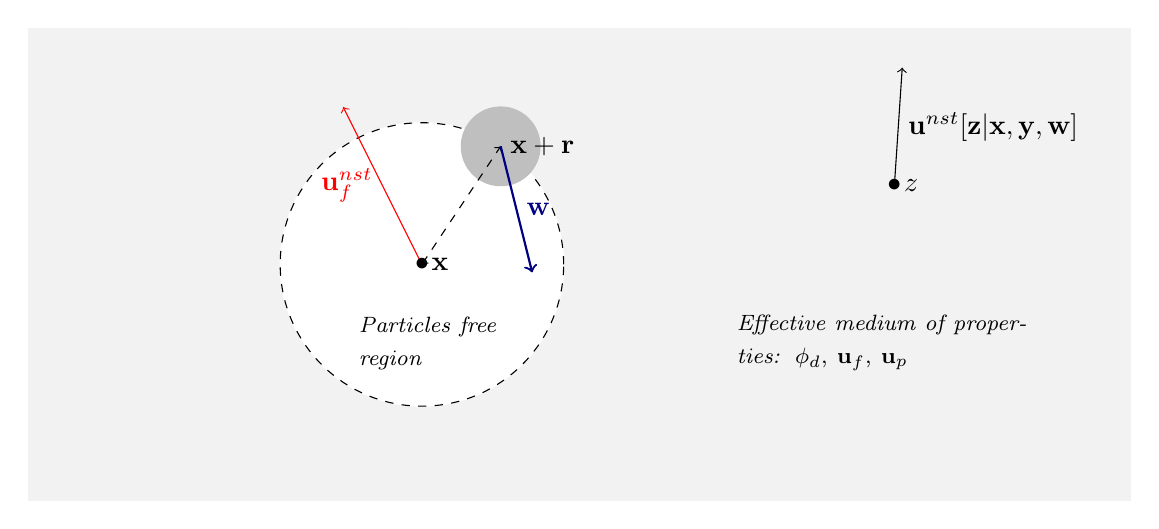
\begin{tikzpicture}
    \filldraw[gray!10](-5,-3) rectangle(9,3);
    \filldraw[white](0,0) circle (1.8);
    \filldraw[ gray!10!white](+2.6,0.5)circle (0.5);
    \filldraw[ gray!10!white](-1.5,2.2)circle (0.5);
    \draw[dashed](0:1.8) arc (0:360:1.8);
    % \filldraw[ gray!50!white](0,0) circle (0.5);
    \filldraw[ gray!50!white](1,1.5)circle (0.5);
    \filldraw[ gray!10!white](-0.2,2.5)circle (0.5);
    \draw[->,red](0,0)--++(-1,2)node[midway,left]{$\textbf{u}_f^\text{nst}$};
    \draw(0,0)node{$\bullet$}node[right]{$\textbf{x}$};
    \draw[dashed,<->](0,0)--(1,1.5)node[right]{$\textbf{x}+\textbf{r}$};
    \draw[->,blue!50!black,thick](1,1.5)--++(0.4,-1.6)node[midway,right]{$\textbf{w}$};
    % \draw[dashed](-0.2,3.5);
    \node[text width=2cm] (title) at (0.2,-1) {\footnotesize\textit{Particles free region}};
    % \node[ultra thick] (title) at (-0.5,-1.5) {(\textit{Case 1})};
    \node[text width=4cm] (title) at (6,-1) {\footnotesize\textit{Effective medium of properties:} $\phi_d$, $\textbf{u}_f$, $\textbf{u}_p$};
    \draw[->] (6,1)node{$\bullet$}node[right]{$z$}--++(0.1,1.5)node[right,midway]{$\textbf{u}^\text{nst}[\textbf{z}|\textbf{x},\textbf{y},\textbf{w}]$};
\end{tikzpicture} 
\caption{Representation of the \textit{nearest neighbor conditionally averaged} velocity fields $\textbf{u}_\text{nst}^f[\textbf{x},\textbf{w},\textbf{r},t]$.
Figure adapted from (Figure 2) of \citet{zhang2021ensemble}}
\label{fig:unst}
\end{figure}
According to \ref{eq:def_f_nst} and \ref{fig:unst} $\textbf{u}_f^\text{nst}[\textbf{x},\textbf{r},\textbf{w}]$ is the averaged value of $\textbf{u}_f^0$, evaluated at \textbf{x}, on all configuration where the nearest droplet is present at $\textbf{y} = \textbf{x} + \textbf{r}$ with velocity $\textbf{w}$. 
Consequently, the region delimited by the sphere, centered at \textbf{x} of radius $|\textbf{y} - \textbf{x}|$ must be empty of particles center of mass since the closest neighboring droplet is at \textbf{y} \citep{zhang2021ensemble}. 
The region outside this particle-free region corresponds therefore to an effective medium where both the particle and the fluid phase are averaged conditionally on the configuration represented by $\chi_f\delta_\text{nst}$. 
This deeper physical understanding will prove valuable in the subsequent section.  
We argue however that the particle-free zone as defined by \ref{fig:unst} is incomplete. 
Indeed, inside the spherical shell of radius $2a$ centered at $\textbf{y}$ no center of mass of droplets can be present due to the impenetrability of the droplets. 
However, we neglect this term for now. 


In summary, we reformulated the ensemble-averaged \textit{Reynolds stress} tensor using a well-normed conditional average \eqref{eq:def_f_nst} based on the nearest particle's position and velocity. 
However, in this phase-space, $\textbf{v}_f^\text{nst}$ is not merely the velocity field around a particle but rather the velocity field averaged over a specific scenario, as illustrated in \ref{fig:unst}. 

\subsection{Equations for the nearest neighbor averaged velocity fields. }

To compute the sedimentation velocity in non-dilute suspensions of hard spheres, \citet[Appendix B]{zhang2021ensemble} derived the field $\textbf{u}_f^\text{nst}$ using the \textit{nearest neighbor conditionally averaged} Navier-Stokes equations. 
% As the derivation lacks detailed proof, particularly regarding the steps leading to Equation (B 1) of \citet{zhang2021ensemble}, 
We present in this section a systematic methodology for deriving these conditionally averaged equations. 

Inspired by the classic conditional average methodology of \citet{hinch1977averaged}, we propose that the \textit{nearest neighbor conditionally averaged} velocity fields, i.e., $\textbf{v}_f^\text{nst}$, can be obtained by conditionally averaging the local-scale mass and momentum equations, and then solving the resulting equations for $\textbf{v}_f^\text{nst}$. 
% Thus, we first recall the local mass and momentum equations, 
% \begin{align}
%     \pddt (\rho_f\chi_f) +  \pddx \cdot (\rho_f\chi_f\textbf{u}^0_f) &= 0 
%     \label{eq:local_equations_mass}
%     \\
%     \pddt (\rho_f\chi_f\textbf{u}^0_f)
%     + \pddx\cdot (\rho_f\chi_f\textbf{u}^0_f\textbf{u}^0_f - \chi_f\bm\sigma^0_f)
%     &= 
%     - \delta_\Gamma \bm\sigma_f^0 \cdot \textbf{n}_d. 
%     + \chi_f \rho_f \textbf{g}
%     \label{eq:local_equations_mom}
% \end{align}
% Note that, at this stage, the inertial terms cannot be neglected since the momentum equation is not yet expressed in the reference frame of the droplet at \textbf{y}. 
Then, note that we can obtain $\textbf{v}_f^\text{nst}$ from $\textbf{u}_f^0$ directly through the averaging procedure: 
\begin{equation}
    \textbf{v}_f^\text{nst} P_\text{nst}^f\phi_f
    = 
    (\textbf{u}_f^\text{nst} P_\text{nst}^f
    - \textbf{u}_f P_\text{nst}^f)\phi_f
    = 
    \avg{(\delta_\text{nst}  - P_\text{nst}^f)\chi_f\textbf{u}_f^0}
\end{equation}
Following the methodology of \ref{chap:daniel2} we deduce that to obtain an equation for $\textbf{v}_f^\text{nst}$ we must multiply the local scale equations evaluated at \textbf{x}, by $(\delta_\text{nst}\chi_f - P_\text{nst}^f\chi_f)$ and average over all configurations. 
This introduces the need for a conservation equation for the distributions $\delta_\text{nst}$ and $P_\text{nst}^f$ since these distributions does not commute with the time and space derivative. 

\subsubsection{Evolution equation for $\delta_\text{nst}$ and  $P_\text{nst}^f$ }

By taking the partial time derivative of each distribution present in \ref{eq:def_delta_nst} independently, we obtain the conservation equations, 
\begin{align}
    \label{eq:dt_delta_x}
    \pddt \delta(\textbf{x}_i  - \textbf{y})
    +\textbf{u}_i  
    \cdot \pddy \delta(\textbf{x}_i  - \textbf{y})
    = 0\\
    \pddt \delta(\textbf{u}_i -\textbf{w})
    +\textbf{a}_i \cdot  \pddw   \delta(\textbf{u}_i  - \textbf{w})
    = 0\\
    \pddt \chi_f 
    + \textbf{u}_\Gamma^0 
    \cdot \pddx \chi_f = 0 \\
    \pddx \chi_f = - \delta_\Gamma \textbf{n}_f,
    \label{eq:chi_f_dt}
\end{align}
where we recall that $\textbf{u}_\Gamma^0$ is the velocity of the droplets interfaces, and $\textbf{n}_f$ is the normal pointing inward the droplets surfaces. 
Additionally, The vector $\textbf{a}_i = \ddt \textbf{u}_i$ corresponds to the center of mass acceleration of the particle $i$. 
From the conservation laws given by \ref{eq:dt_delta_x} to \ref{eq:chi_f_dt}, we deduce that, 
\begin{align}
    \pddt \delta_\text{nst}
    + \pddy \cdot (\textbf{w} \delta_\text{nst})
    + \pddw \cdot (\textbf{a}_i  \delta_\text{nst})
    = 
    \sum_i \delta(\textbf{x}_i -\textbf{y}) \delta(\textbf{u}_i - \textbf{w}) \pddt h_i
\end{align}
% and, 
% \begin{align*}
%     \pddt (\chi_f \delta_\text{nst})
%     + \pddy \cdot (\textbf{w} \chi_f \delta_\text{nst})
%     + \pddw \cdot (\textbf{a}_i  \chi_f \delta_\text{nst})
%     = 
%     \chi_f \delta(\textbf{x}_i -\textbf{y}) \delta(\textbf{u}_i - \textbf{w}) \pddt h_i
%     + \delta_\Gamma \delta_\text{nst} \textbf{u}_\Gamma\cdot \textbf{n}_f
% \end{align*}
Additionally, it can be shown that,
\begin{align}
    \pddt  h_i[\textbf{x},t,\FF]
    = 
    h_i
    \sum_k 
    \delta(r_k - r_i)
    (\textbf{u}_k  \cdot \hat{\textbf{r}}_k - \textbf{u}_i  \cdot \hat{\textbf{r}}_i)\\
    \pddx  h_i[\textbf{x},t,\FF]
    = 
    h_i
    \sum_k 
    \delta(r_k - r_i)
    ( \hat{\textbf{r}}_k -  \hat{\textbf{r}}_i),
    \label{eq:dt_h_i}
\end{align}
where $\textbf{u}_k$ and $\textbf{u}_i$  are the center of mass velocity of the particle $k$ and $i$, respectively.
Note that the second expression agrees with \citet[Appendix A]{zhang2021ensemble}. 
We also introduced the notation $r_i$ and $r_k$ which represents the radial distance from the particle $i$ to the point $\textbf{x}$ namely, $r_i = |\textbf{x}_i - \textbf{x}|$.  
Considering \ref{eq:dt_h_i}  yields an expression for the transport equation of $\delta_\text{nst}$ namely,
\begin{equation}
    \pddt \delta_\text{nst}
    + \pddy \cdot (\textbf{w} \delta_\text{nst})
    + \pddw \cdot (\textbf{a}_i  \delta_\text{nst})
    = 
    % \sum_i
    % \delta(\textbf{x}_i -\textbf{y}) 
    % \delta(\textbf{u}_i - \textbf{w}) 
    \delta_\text{nst}
    % h_i
    \sum_k 
    \delta(r_k - r_i)
    (\textbf{u}_k  \cdot \hat{\textbf{r}}_k - \textbf{u}_i  \cdot \hat{\textbf{r}}_i). 
    \label{eq:dt_delta_nst_start}
\end{equation}
As demonstrated in \citet{zhang2023evolution}, the right-hand side term of \ref{eq:dt_delta_nst_start} represents the source terms due to the permutation of nearest neighbor to the point \textbf{x}. 
For reasons that will become clear later on, we add the term $\textbf{u}_f^0\cdot \pddx \delta_\text{nst}$ on each side of \ref{eq:dt_delta_nst_start}, which gives,
\begin{equation}
    \pddt \delta_\text{nst}
    + \textbf{u}_f^0\cdot \pddx \delta_\text{nst}
    + \textbf{w}   \cdot \pddy \delta_\text{nst}
    + \textbf{a}_i \cdot \pddw   \delta_\text{nst}
    = 
    % \sum_i
    % \delta(\textbf{x}_i -\textbf{y}) 
    % \delta(\textbf{u}_i - \textbf{w}) 
    \delta_\text{nst}
    % h_i
    \sum_k 
    \delta(r_k - r_i)
    [(\textbf{u}_k - \textbf{u}_f^0) \cdot \hat{\textbf{r}}_k - (\textbf{u}_i  - \textbf{u}_f^0)\cdot \hat{\textbf{r}}_i]. 
    \label{eq:dt_delta_nst}
\end{equation}
Where on the right-hand side of \ref{eq:dt_delta_nst} we have reformulated the term $\textbf{u}_f^0\cdot \pddx \delta_\text{nst}$, using \ref{eq:dt_h_i}. 

To derive an equation for $\phi_f P_\text{nst}^f = \avg{\chi_f \delta_\text{nst}}$ we multiply \ref{eq:dt_delta_nst} by $\chi_f$, and use \ref{eq:chi_f_dt}, namely
\begin{multline}
    \pddt (\chi_f\delta_\text{nst})
    +  \pddx \cdot (\textbf{u}_f^0 \chi_f\delta_\text{nst})
    +  \pddy \cdot (\textbf{w}    \chi_f\delta_\text{nst})
    +  \pddw \cdot   (\textbf{a}_i  \chi_f\delta_\text{nst})\\
    = 
    % \sum_i
    % \delta(\textbf{x}_i -\textbf{y}) 
    % \delta(\textbf{u}_i - \textbf{w}) 
    (\chi_f\delta_\text{nst})
    % h_i
    \sum_k 
    \delta(r_k - r_i)
    [(\textbf{u}_k - \textbf{u}_f^0) \cdot \hat{\textbf{r}}_k - (\textbf{u}_i  - \textbf{u}_f^0)\cdot \hat{\textbf{r}}_i],
    \label{eq:dt_delta_nst_chi}
\end{multline}
which upon averaging directly gives,
\begin{multline}
    \pddt (\phi_fP_\text{nst}^f)
    + 
    \pddx \cdot (
        \phi_f 
        P_\text{nst}^f
        \textbf{u}_f^\text{nst}
    )
    + \pddy \cdot (
        \phi_f
        P_\text{nst}^f
        \textbf{w} 
    )
    +
    \pddw \cdot (  
        \phi_f 
        P_\text{nst}^f
        \textbf{a}_p^\text{nst} 
    )
    = \\
    + \avg{
    %  \chi_f \textbf{u}_\Gamma \cdot \pddx \delta_\text{nst}
     \chi_f \delta_\text{nst}
    \sum_k 
    \delta(r_k - r_i)
    [(\textbf{u}_k - \textbf{u}_\Gamma^0) \cdot \hat{\textbf{r}}_k - (\textbf{u}_i- \textbf{u}_\Gamma^0)  \cdot \hat{\textbf{r}}_i]}.
    \label{eq:dt_P_nst_chi}
\end{multline}
% where we have noted that $\textbf{u}_\Gamma^0 = \textbf{u}_f^0$ in the absence of mass transfer. 
In this relation, the left-hand side terms represent the advection of $\phi_f P_\text{nst}^f$ along the phase space variables ($t$, $\textbf{x}$, $\textbf{y}$ and $\textbf{w}$).
The source term on the right-hand side of \ref{eq:dt_P_nst_chi} accounts for the changes in nearest neighbor distribution due to the permutation of the nearest neighbor at the local scale. 
Note the similarities of the right-hand side source term of \ref{eq:dt_P_nst_chi} with (A10) of \citet{zhang2023evolution}, which derived a transport equation for $P_\text{nst}$, which is defined as the probability density of the nearest pairs of particles as it is described in \ref{chap:microstructure}. 
We remark that the source terms of (A10) \citet{zhang2023evolution} and \ref{eq:dt_P_nst_chi} yield the same form.
Still in \ref{eq:dt_P_nst_chi} the velocity $\textbf{u}_i$ and $\textbf{u}_k$ are evaluated with respect to the local velocity of the fluid $\textbf{u}_f^0$, while in \citet{zhang2023evolution} it is evaluated relative to the velocity of the particles centered at \textbf{x}. 


% \ref{eq:dt_P_nst_chi} can also be written in ``conservative'' form using the conserving law, 
% \begin{equation}
%     \pddt \phi_f 
%     + \div(
%         \phi_f
%         \textbf{u}_f 
%         ) 
%     = 0, 
% \end{equation}
% which gives, 
% \begin{multline}
%     \pddt P_\text{nst}^f
%     + 
%     \pddx \cdot (
%         P_\text{nst}^f
%         \textbf{u}_f^\text{nst}
%     )
%     + \pddy \cdot (
%         P_\text{nst}^f
%         \textbf{w}
%     )
%     +
%     \pddw \cdot (  
%         P_\text{nst}^f
%         \textbf{a}_p^\text{nst} 
%     )
%     = \\
%     + \frac{1}{\phi_f}\avg{
%     %  \chi_f \textbf{u}_\Gamma \cdot \pddx \delta_\text{nst}
%      \chi_f \delta_\text{nst}
%     \sum_k 
%     \delta(r_k - r_i)
%     [(\textbf{u}_k - \textbf{u}_\Gamma^0) \cdot \hat{\textbf{r}}_k - (\textbf{u}_i- \textbf{u}_\Gamma^0)  \cdot \hat{\textbf{r}}_i]}.
%     \label{eq:dt_Pc_nst_chi}
% \end{multline}
% this equation corresponds to the \textit{nearest neighbor conditional averaged} conservation equation for the continuous phase.
% As the continuous phase density $\rho_f$ is constant, \ref{eq:dt_Pc_nst_chi} also corresponds to the  \textit{nearest neighbor conditional averaged} mass conservation equation.  

% \subsubsection{First form of the conditional averaged momentum equation}
% Now that the transport equation for $\delta_\text{nst}$ and $P_\text{nst}^f$ are properly derived we can derive the \textit{nearest neighbor conditionally averaged} momentum equation. 
% Multiplying \ref{eq:local_equations_mom} by $\delta_\text{nst}$, and making use of \ref{eq:dt_delta_nst} and averaging overall configurations yields, 
% \begin{multline}
%     \pddt (\rho_f\phi_f P_\text{nst} \textbf{u}^\text{nst}_f)
%     + \pddx\cdot (
%         \rho_f\phi_fP_\text{nst}^f \textbf{u}^\text{nst}_f\textbf{u}^\text{nst}_f 
%         +\bm\sigma_\text{nst}^\text{eq})
%     + \pddy\cdot (\phi_fP_\text{nst}^f \textbf{w}\textbf{u}_f^\text{nst} )
%     + \pddw\cdot (\phi_fP_\text{nst}^f \textbf{a}_p^\text{nst} \textbf{u}_f^\text{nst} )\\
%     = 
%     \phi_fP_\text{nst}^f  \rho_f \textbf{g}
%     - \avg{\delta_\text{nst}\delta_\Gamma \bm\sigma_f \cdot \textbf{n}_d} 
%     % - \avg{\chi_f \bm\sigma_f^0 \cdot \grad\delta_\text{nst}}
%     +\avg{
%         \delta_\text{nst}
%         \chi_f \bm\sigma_f^0 \cdot
%         \sum_k 
%         \delta(r_k - r_i)
%         [\hat{\textbf{r}}_k - \hat{\textbf{r}}_i]}\\
%     +\avg{
%         %  \chi_f \textbf{u}_\Gamma \cdot \pddx \delta_\text{nst}
%          \textbf{u}_f^0\chi_f \delta_\text{nst}
%         \sum_k 
%         \delta(r_k - r_i)
%         [(\textbf{u}_k - \textbf{u}_f^0) \cdot \hat{\textbf{r}}_k - (\textbf{u}_i- \textbf{u}_f^0)  \cdot \hat{\textbf{r}}_i]},
%     \label{eq:momentum_avg_nst}
% \end{multline}
% with the effective stress $\bm\sigma_\text{nst}^\text{eq}$ defined as, 
% \begin{equation}
%     \bm\sigma_\text{nst}^\text{eq}=
%     \avg{\rho_f\chi_f\delta_\text{nst} \textbf{u}''_f\textbf{u}''_f} 
%     - P_\text{nst}^f \avg{\rho_f\chi_f\textbf{u}'_f\textbf{u}'_f} 
%     - \phi_f P_\text{nst}^f \bm\sigma^\text{nst}_f. 
% \end{equation}
% The terms on the left-hand side of \ref{eq:momentum_avg_nst} represent the advection of the \textit{nearest neighbor conditional average} momentum along the phase space coordinate, plus the contribution of the \textit{nearest neighbor conditional average} viscous stresses $\bm\sigma^\text{nst}_f$
% The first term on right-hand side of \ref{eq:momentum_avg_nst} corresponds to the momentum exchange between phases, but conditionally averaged. 
% Specifically, $\avg{\delta_\text{nst}\delta_\Gamma \bm\sigma_f \cdot \textbf{n}_d} $ represents the exchange of momentum at \textbf{x}, conditioned on the presence of the interface at \textbf{x} with the nearest neighbor to the point \textbf{x} located at \textbf{y} with velocity \textbf{w}.
% The second and third terms are the additional contribution of the convective and non-convective fluxes due to the birth or death of nearest neighbors. 

% In this form \ref{eq:momentum_avg_nst} is hardly solvable. 

\subsubsection{Conditional averaged momentum equations}

While, the boundary condition at the surface of the particle (centered at \textbf{y}) for the velocity $\textbf{u}_f^\text{nst}[\textbf{y}+a \textbf{n}, \textbf{y},\textbf{w}]$ is well-defined, there is a lack of boundary conditions infinitely far from the particle. 
Indeed, since the velocity field $\textbf{u}_f^\text{nst}$ is conditioned on the velocity of the droplet, we can be certain that $\textbf{u}_f^\text{nst}\cdot \textbf{n} = \textbf{w}\cdot \textbf{n}$ for the points lying on the droplet surface. 
However, $\lim_{|\textbf{x}- \textbf{y}|\to \infty} \textbf{u}^\text{nst}_f$ is undefined, since in the same limits $P_\text{nst}^f = 0$.
In other words, infinitely far from the particle's center of mass, the velocity field $\textbf{u}^\text{nst}_f$ has no physical meaning, because the probability of finding the nearest neighbor to a point in the fluid at such a distance is zero.
% This, lack of boundary condition at infinity makes, \ref{eq:momentum_avg_nst} unsolvable regardless of the possible assumption that could be made.


To settle this issue we follow \citet[Appendix B]{zhang2021ensemble} and propose to solve for an auxiliary but equivalent problem.
Indeed, as $\textbf{u}_f^\text{nst}$ lacks a boundary condition at infinity, we choose instead to solve for the field $\textbf{u}^\text{nst}$ which is defined as,  
\begin{equation*}
    P_\text{nst-f}[\textbf{y},\textbf{w},\textbf{x},t]\textbf{u}^\text{nst}[\textbf{z},t|\textbf{x},\textbf{y},\textbf{w}]
    = \avg{\delta_\text{nst-f}  \textbf{u}^0[\textbf{z},\FF,t]}
    \label{eq:def_u_z}
\end{equation*}
where, $\delta_\text{nst-f} = \chi_f[\textbf{x},t,\FF]\delta_\text{nst}[\textbf{y},\textbf{w}, \FF,t]$. 
We recall that $\textbf{u}^0 = \chi_f\textbf{u}_f^0 + \chi_d \textbf{u}_d^0$ is the local bulk velocity of the mixture. 
Additionally, $P_\text{nst-f}$ is defined as,
\begin{equation}
    P_\text{nst-f}[\textbf{x},\textbf{y},\textbf{w},t] = \phi_f[\textbf{x},t]P_\text{nst}^f[\textbf{y},\textbf{w},t|\textbf{x}] = \avg{\delta_\text{nst-f}}. 
\end{equation}
Note that we included the subscript $f$ in $P_\text{nst-f}$ to indicate that the probability distribution $\phi_f$ is not a condition but is rather part of the distribution $P_\text{nst-f}$.
Thus, $\textbf{u}^\text{nst}$ is the \textit{nearest neighbor conditionally averaged} bulk velocity field evaluated at $\textbf{z}$, knowing the fluid phase is present at $\textbf{x}$ with the nearest neighbor to \textbf{x} being located in \textbf{y} with center of mass velocity \textbf{w}. 
A graphical representation of $\textbf{u}^\text{nst}$ is given in \ref{fig:unst}.
With that definition, we have the following boundary condition far from the particle-free region, 
\begin{equation}
    \lim_{|\textbf{z} - \textbf{y}|\to \infty}
    \textbf{u}^\text{nst}[\textbf{z},t|\textbf{x},\textbf{y},\textbf{w}]
    = \textbf{u}[\textbf{z},t]. 
    % \lim_{|\textbf{z} - \textbf{y}|\to \infty}
    % \phi^\text{nst}[\textbf{z},t|\textbf{x},\textbf{y},\textbf{w}]
    % = \phi[\textbf{z},t],
    \label{eq:boundary}
\end{equation}
We recall that $\textbf{u} = \avg{\chi_f\textbf{u}_f^0 + \chi_d \textbf{u}_d^0}$. 
\ref{eq:boundary} indicates that, far from the particle-free region, the particle located at \textbf{y} has no influence on the averaged quantities.
Additionally, note that, $\textbf{u}^\text{nst}$ is related to $\textbf{u}_f^\text{nst}$ such that, $\textbf{u}^\text{nst}[\textbf{x},t|\textbf{x},\textbf{y},\textbf{w}] = \textbf{u}_f^\text{nst}[\textbf{x},\textbf{y},\textbf{w},t]$ since only the fluid phase is present at \textbf{x} by definition. 
Therefore, $\textbf{u}^\text{nst}$ possesses the advantageous property of having well-defined boundary conditions at large distances from the particle center, and is equivalent to $\textbf{u}_f^\text{nst}$ (which is required in \ref{eq:relation_ensemble_nst}) when evaluated at \textbf{x}. 


Now, we introduce the disturbance fields $\textbf{v}^\text{nst} = \textbf{u}^\text{nst} - \textbf{u}$, which, according to  \ref{eq:boundary}, satisfy the condition
\begin{equation}
    \lim_{|\textbf{z} - \textbf{y}|\to \infty}
    \textbf{v}^\text{nst}[\textbf{z},t|\textbf{x},\textbf{y},\textbf{w}]
    = 0,
\end{equation}
while the boundary condition at the surface of the particle is given by, 
\begin{equation}
    \textbf{v}^\text{nst}\cdot \textbf{n}
    = 
    (\textbf{w} - \textbf{u}[\textbf{z},t])\cdot \textbf{n}
    = 
    \left\{
        \textbf{w}
        - \textbf{u}[\textbf{y},t]
        - (\textbf{y} - \textbf{z})\cdot \grad\textbf{u}|_{\textbf{z}=\textbf{y}}
        + \ldots 
    \right\}
    \;\;\; \forall \textbf{z}\in \left\{ |\textbf{z} - \textbf{y}| = a  \right\}. 
    \label{eq:bounday2}
\end{equation}
The second equality is obtained by expanding $ \textbf{u}[\textbf{z},t]$ in a Taylor expansion around the point \textbf{y}. 
Since, $\textbf{v}^\text{nst} = 0$ far from the particle at \textbf{y}, we can state that  $\textbf{v}^\text{nst}$ is a ``disturbance field'', that is conditioned by the presence of a droplet at \textbf{y} that is the nearest neighbor to a point \textbf{x} in the fluid. 
Note that these boundary conditions, as well as those derived in \ref{chap:daniel2} for the Single-point conditionally averaged Navier-Stokes equations, are exactly the same but applied to the bulk velocity rather than the continuous phase velocity.

Since, the boundary condition at the surface of the particle involves the bulk velocity $\textbf{u}$, we use the \textit{single-fluid} formulation of the local mass and momentum conservation equations. 
We recall their form here : 
\begin{align}
    \pddz \cdot \textbf{u}^0 = 0 \\
    \pddt (\rho^0\textbf{u}^0)
    + \pddz\cdot 
    (\rho^0\textbf{u}^0\textbf{u}^0 
    -\bm\sigma^0)
    &= 
    + \rho^0 \textbf{g}. 
    \label{eq:local_equations_bulk}
\end{align}
To obtain the \textit{nearest neighbor conditionally averaged} Navier-Stokes equations for the disturbance field  $\textbf{v}^\text{nst}$, we multiply \ref{eq:local_equations_bulk} by $(\delta_\text{nst-f} - P_\text{nst-f})$ and average overall configurations.
We recall that \ref{eq:local_equations_bulk} is evaluated at the point \textbf{z}, which is independent of \textbf{x} or \textbf{y}. 
Therefore, since $(\delta_\text{nst-f} - P_\text{nst-f})[\textbf{x},\textbf{y},\textbf{w},t]$ is not a function of \textbf{x} the mass conservation directly gives, 
\begin{equation}
    \pddz \cdot \avg{(\delta_\text{nst-f} - P_\text{nst-f}) \textbf{u}^0}
    = 0. 
    \label{eq:mass_nst_d}
\end{equation}
As the time derivative and $(\delta_\text{nst-f} - P_\text{nst-f})$ do not commute, the momentum equation is obtained by using \ref{eq:dt_delta_nst_chi} and \ref{eq:dt_P_nst_chi}, which gives, 
\begin{multline}
    \pddt \avg{(\delta_\text{nst-f} - P_\text{nst-f})\rho^0\textbf{u}^0}
    + \pddz\cdot \avg{ (\delta_\text{nst-f} - P_\text{nst-f}) ( \rho^0  \textbf{u}^0 \textbf{u}^0 - \bm\sigma^0)}\\
    +  \pddx \cdot \avg{(\delta_\text{nst-f} \textbf{u}_f^0 - P_\text{nst-f}\textbf{u}_f^\text{nst}) \rho^0 \textbf{u}^0}
    +  \pddy \cdot \avg{(\delta_\text{nst-f} - P_\text{nst-f}) \textbf{w} \textbf{u}^0 \rho^0}\\
    +  \pddw \cdot \avg{(\delta_\text{nst-f} \textbf{a}_i - P_\text{nst-f} \textbf{a}_p^\text{nst})\textbf{u}^0 \rho^0 }
    = 
    % - \avg{(\delta_\text{nst-f} - P_\text{nst-f})\delta_\Gamma \bm\sigma_f^0 \cdot \textbf{n}_d }
     \avg{(\delta_\text{nst-f} - P_\text{nst-f})\rho^0 \textbf{g}} 
    + 
    \avg{\rho^0 \textbf{u}^0 S'_\text{nst} },
    \label{eq:momentum_nst_d}
\end{multline}
where we have defined $S_\text{nst}'$ as the source change of momentum generated by permutation of nearest neighbors to the point \textbf{x}, that is,
\begin{multline}
    S_\text{nst}'
    =
    \left\{
    \delta_\text{nst-f}
        % h_i
        \sum_k 
        \delta(r_k - r_i)
        ((\textbf{u}_k - \textbf{u}_f^0) \cdot \hat{\textbf{r}}_k - (\textbf{u}_i  - \textbf{u}_f^0)\cdot \hat{\textbf{r}}_i) 
    - \right.\\ \left.
    \avg{
         \delta_\text{nst-f}
        % h_i
        \sum_k 
        \delta(r_k - r_i)
        ((\textbf{u}_k - \textbf{u}_f^0) \cdot \hat{\textbf{r}}_k - (\textbf{u}_i  - \textbf{u}_f^0)\cdot \hat{\textbf{r}}_i) 
    }
    \right\}. 
\end{multline}
In this general form, these equations may appear complex; thus, we will now provide a detailed explanation of the meaning of each term.

We start by the \textit{nearest-neighbor conditional averaged} mass conservation equation \eqref{eq:mass_nst_d}. 
By definition, we have, 
\begin{equation}
    \avg{(\delta_\text{nst-f} - P_\text{nst-f} )\textbf{u}^0}
    = P_\text{nst-f} (\textbf{u}^\text{nst} - \textbf{u})
    = P_\text{nst-f} \textbf{v}^\text{nst}. 
\end{equation}
Since $P_\text{nst}$ is not a function of \textbf{z}, \ref{eq:mass_nst_d} reduce to $\div\textbf{v}^\text{nst}=0$.
Thus, we have demonstrated that the non-trivial disturbance field $\textbf{v}^\text{nst}$ remains divergence-free, irrespective of the flow regime.

Regarding the \textit{nearest neighbor conditionally averaged} equations \eqref{eq:momentum_nst_d} we may reformulate the first term on the left-hand side as, 
\begin{equation}
    \avg{(\delta_\text{nst-f} - P_\text{nst-f})\rho^0 \textbf{u}^0}
    = P_\text{nst-f} [
        \rho^\text{nst}\textbf{u}_m^\text{nst}
        - 
        \rho \textbf{u}_m
    ]
    = P_\text{nst-f} [
        \rho^\text{nst-d}\textbf{v}^\text{nst}_m
        + \rho^\text{nst-d}\textbf{u}_m
        + \rho \textbf{v}^\text{nst}_m
    ]
\end{equation}
where we recall that $\rho \textbf{u}_m = \avg{\rho_f\chi_f \textbf{u}_f + \rho_d\chi_f  \textbf{u}_d}$ is the weighted or Favre average.
Likewise, $\rho^\text{nst} \textbf{u}_m^\text{nst} = \avg{\delta_{nst-f}(\rho_f\chi_f \textbf{u}_f + \rho_d\chi_f  \textbf{u}_d)}$ is the conditional Favre average of the velocity. 
We introduced the superscript $^{-d}$ on $\rho^\text{nst-d} = \rho^\text{nst} - \rho$ to indicate that $\rho^\text{nst-d}$ is a disturbance field that vanishes at large distances  $|\textbf{z} - \textbf{y}|$, similar to the condition in \ref{eq:boundary} for the velocity field $\textbf{v}^\text{nst}$. 
Thus, the first term on the left-hand side of \ref{eq:momentum_nst_d} is the time derivative of the disturbance momentum field. 
We deduce that \ref{eq:momentum_nst_d} is a conservation equation for the disturbance momentum field.
Thus, the remaining terms on the left-hand side of \ref{eq:momentum_nst_d} correspond to the advective terms over the phase space coordinates.
And finally the last term is the \textit{nearest neighbor conditionally averaged} disturbance stress,  
\begin{equation}
    \avg{(\delta_\text{nst-f} - P_\text{nst-f}) \bm\sigma^0}
    = P_\text{nst-f} (\bm\sigma^\text{nst} - \bm\sigma)
    = P_\text{nst-f} \bm\sigma^\text{nst-d}
\end{equation}
Note that since both fluids are considered Newtonian $\bm\sigma_k^0 = -p_k^0\bm\delta + \mu_k (\grad \textbf{u}_k^0 + \grad \textbf{u}_k^0)$, therefore we write,
\begin{align}
    \avg{(\delta_\text{nst-f} - P_\text{nst-f}) \bm\sigma^0}
    % &=
    % \avg{(\delta_\text{nst-f} - P_\text{nst-f}) 
    % \left[
    % - p^0 \bm\delta 
    % + \mu_f(\grad \textbf{u}^\dagger + (\grad \textbf{u}^0)^\dagger )
    % + \chi_d (\mu_d-\mu_f)\textbf{e}_d^0 
    % + \delta_\Gamma \gamma (\bm\delta - \textbf{nn})
    % \right]
    % }\nonumber \\
    &=
    P_\text{nst-f}\left\{
        -p^\text{nst-d}\bm\delta 
        + \mu_f [\pddz \textbf{u}^\text{nst-d}+^\dagger\pddz \textbf{u}^\text{nst-d}]
    \right\}\nonumber\\
   &+  \avg{(\delta_\text{nst-f} - P_\text{nst-f})[
    \chi_d  2 (\mu_d-\mu_f)\textbf{e}_d^0 
    + \delta_\Gamma \gamma (\bm\delta - \textbf{nn})]
    }
    \label{eq:stress_nst}
\end{align}
The terms on the first line on the right-hand side correspond to the mean fluid phase stress, with the mean disturbance pressure, $p^\text{nst-d}$ and the mean disturbance shear rate $\mu_f [\pddz \textbf{u}^\text{nst-d}+^\dagger\pddz \textbf{u}^\text{nst-d}]$. 
The terms on the second line represent the particle contribution to the mixture stresses, including surface tension effects and particle internal shear rate. 
Note that both parts of the stresses satisfy the property to vanish at a large distance to the particle-free zone.

Finally, on the right-hand side of \ref{eq:momentum_nst_d} we find the disturbance source terms related to the buoyancy force, namely,
\begin{equation*}
    \avg{(\delta_\text{nst} - P_\text{nst-f}) \chi_f \rho^0 \textbf{g}}
    = 
    P_\text{nst-f} \rho^\text{nst-d} \textbf{g}. 
\end{equation*}
More details will be given in the next section regarding this contribution. 

To summary, \ref{eq:mass_nst_d} and \ref{eq:momentum_nst_d} together with the boundary conditions formed by \ref{eq:boundary} and \ref{eq:bounday2}, constitute a system of conditionally averaged equation, to be solved for the disturbance velocity fields, $\textbf{v}^\text{nst}[\textbf{z},t|\textbf{x},\textbf{y},\textbf{w}]$ and the disturbance density, $\rho^\text{nst-d}[\textbf{z},t|\textbf{x},\textbf{y},\textbf{w}]$.
However, due to the complexity of the problem, arising due to the consideration of a phase space with  13 dimensions ($\textbf{z},t,\textbf{x},\textbf{y},\textbf{w}$), we must now consider some simplifying hypothesis.

\subsection{Simplifying assumptions}

Due to the challenging theoretical nature of the problem, we must make several simplifying assumptions. 
Specifically, we consider a stationary, inertialess scenario, meaning that we neglect the time derivatives and advective terms in \ref{eq:mass_nst_d} and \ref{eq:momentum_nst_d}. 
The advective terms in \ref{eq:momentum_nst_d} are all proportional to $\textbf{v}^\text{nst}\textbf{v}^\text{nst}$, which is itself proportional to the relative velocity between the particle and the continuous phase. Consequently, these terms are of $\mathcal{O}(Re)$ or higher, where $Re$ represents the Reynolds number based on the relative phase velocity.
Likewise, we will assume a dilute regime, meaning that we neglect all terms of $\mathcal{O}(\phi)$ or higher. Finally, we assume the suspension is homogeneous, implying that the ensemble-averaged quantities are uniform and do not depend on $\textbf{z}$.
Consequently, $\textbf{u}[\textbf{z},t] = \textbf{u}[\textbf{y}]$ in \ref{eq:boundary}. 


At $\mathcal{O}(\phi)$ in the particle-free-region, $\rho^\text{nst} = \rho_f$, and outside the particle-free region $\rho^\text{nst} = \phi_d\rho_d + \phi_f\rho_f= \rho$.
Indeed, outside the particle-free region we consider the values of the effective medium according to \ref{fig:unst}. 
Consequently, the density disturbance fields, $\rho^\text{nst-d}$, has the following form in the dilute regime, 
\begin{equation*}
    \rho^\text{nst-d}[\textbf{z},t|\textbf{x},\textbf{y},\textbf{w}]
    = \phi_d (\rho_f - \rho_d) H(|\textbf{y} - \textbf{x}| - |\textbf{z} - \textbf{x}|).
\end{equation*}
Note that this definition applies only to the points \textbf{z} exterior to the particle. 
Inside the particle, we consider the Stokes equations for single-phase flows of viscosity $\mu_d$. 
Therefore, the buoyancy source term in \ref{eq:momentum_nst_d} is given by, 
\begin{equation*}
    \avg{(\delta_\text{nst} - P_\text{nst-f}) \chi_f \rho_f \textbf{g}}
    = 
    P_\text{nst-f} [\textbf{x},\textbf{y},\textbf{w},t]
    \phi_d[\textbf{z},t] 
    \textbf{g}
    (\rho_f - \rho_d) H(|\textbf{y} - \textbf{x}| - |\textbf{z} - \textbf{x}|), 
\end{equation*}
When $|\textbf{z} - \textbf{y}| > a$. 
Note that in a uniform and steady-state medium $\phi_d[\textbf{z},t] = \phi$ is constant. 


The source term $S_\text{nst}'$ is hard to model, however it seems that it is negligible at $\mathcal{O}(\phi)$ \citet{zhang2021ensemble}. 
Indeed, this term is non-zero only when a second-nearest neighbor is present, meaning that it is proportional to a pair probability density, which is of $\mathcal{O}(\phi)$ higher than the other terms. 

The terms on the second line of the averaged stress \eqref{eq:stress_nst} can be written in the hybrid form as, 
\begin{multline}
    {\chi_d  2 (\mu_d-\mu_f)\textbf{e}_d^0 
    + \delta_\Gamma \gamma (\bm\delta - \textbf{nn})}\\
    \approx
    \frac{1}{2}
     \delta_\alpha\intS{
        \left[(\textbf{r}\bm\sigma_f^0 
        + \bm\sigma_f^0 \textbf{r}
        - \frac{2}{3}\bm\sigma_f^0 \cdot \textbf{r}
        )\cdot \textbf{n} 
        - 2\mu_f (
            \textbf{u}_f^0 \textbf{n}
            + \textbf{n}\textbf{u}_f^0 
        )\right]
    }
    + \div[\ldots],
    \label{eq:stressletalphase}
\end{multline}
where we have not written explicitly the higher order moments. 
Note that the term on the right-hand side of \ref{eq:stressletalphase} corresponds exactly to the Stresslet on the droplet $\alpha$.
The term with the $[\ldots]$ represent the higher order moments of force on this droplet. 
According to \ref{fig:unst} we can assume by completely neglecting the particle interaction that, 
\begin{multline}
    \avg{(\delta_\text{nst-f} - P_\text{nst-f})[\chi_d  2 (\mu_d-\mu_f)\textbf{e}_d^0 
    + \delta_\Gamma \gamma (\bm\delta - \textbf{nn})]} \\
    \approx
    % -\frac{1}{2}
    %  \pSavg{
    %     \left[(\textbf{r}\bm\sigma_f^0 
    %     + \bm\sigma_f^0 \textbf{r}
    %     - \frac{2}{3}\bm\sigma_f^0 \cdot \textbf{r}
    %     )\cdot \textbf{n} 
    %     - 2\mu_f (
    %         \textbf{u}_f^0 \textbf{n}
    %         + \textbf{n}\textbf{u}_f^0 
    %     )\right]
    % }
    % H(|\textbf{y}- \textbf{x}| - |\textbf{z} -\textbf{x}|) \\
    = \{
        -\textbf{S}_p[\textbf{z},t]
        H(|\textbf{y}- \textbf{x}| - |\textbf{z} -\textbf{x}|)
        +
        \frac{1}{2}\div[\textbf{S}_p^{(2)}[\textbf{z},t]H(|\textbf{y}- \textbf{x}| - |\textbf{z} -\textbf{x}|)]\}\\
    + 
    \{
        -(\textbf{S}_p)^\text{nst}[\textbf{y},t]
        \delta(\textbf{z}-\textbf{y})
        +\frac{1}{2}\div[\delta(\textbf{z}-\textbf{y})(\textbf{S}_p^{(2)})^\text{nst}[\textbf{y},t]]
    \}
    + \ldots.
    % \\
    % &- \pddz \cdot \left[
    %     \intS{
    %     \textbf{rr}(\bm\sigma_f^0 \cdot \textbf{n} )}
    %     - 2\mu_f\intO{\textbf{re}_d^0}
    % \right]
    \label{eq:equivalent_stress2NST}
\end{multline}
The contributions present on the second line of \ref{eq:equivalent_stress2NST} correspond to the contribution of the particle-free zone. 
We have introduced the notation $\textbf{S}_p$ and $\textbf{S}_p^{(2)}$ for the ensemble-averaged first and second moment of the hydrodynamic forces on the droplets. 
As we have neglected the droplet-droplet interactions only the value of the ensemble-averaged moments of force remain. 
In stokes flow regime it is clear that $\textbf{S}_p \sim  \phi \mu_f \textbf{e}$ and $\textbf{S}_p^{(2)} \sim  \phi \mu_f (\textbf{u}_p - \textbf{u}_f)\bm\delta$.
However, we do not consider the mean shearing motion in this problem so that $\textbf{e}=0$, $\textbf{S}_p$ is therefore negligible. 
However, $\textbf{S}_p^{(2)}$ isn't null and might not be negligible in this scenario. 
Nevertheless, in the following, we neglect this contribution since for reason that will become clear latter this contribution will turns out to be negligible as well.  

Likewise, $(\textbf{S}_p)^\text{nst}$ and $(\textbf{S}_p^{(2)})^\text{nst}$ correspond to the first and second moment of forces generated by the droplet positioned at $\textbf{y}$. 
In other words $(\textbf{S}_p)^\text{nst}$ and $(\textbf{S}_p^{(2)})^\text{nst}$ represent the response from the droplet surface boundary condition to the flow. 
% For example $(\textbf{S}_p^{(2)})^\text{nst}$ represents the degenerate quadrupole that is present to ensure the no-slip boundary condition for a spherical solid particle in translation in an unbounded Stokes flow. 
Additionally, due to the particle-free zone induced motions, the droplet at \textbf{y} will experience not only a uniform ``background flow'' but also linear and quadratic contributions. 
These moments can be computed using a method similar to the method of reflection \citep{kim2013microhydrodynamics}. 
However, in this case, one must perform a single reflection between the droplet and the flow induced by the particle-free zone (instead of another droplet in the classic method). 
Although these terms are important to ensure that the boundary condition at the surface of the droplet is respected they turn out to be negligible in the final of the Reynolds stress. 



Finally, according to \ref{eq:stress_nst} and the above hypothesis, the disturbance stress might be written, 
\begin{equation}
    \avg{(\delta_\text{nst-f} - P_\text{nst-f}) \bm\sigma^0}
    =
    P_\text{nst-f}\left\{
        -p^\text{nst-d}\bm\delta 
        + \mu_f [\pddz \textbf{u}^\text{nst-d}+^\dagger\pddz \textbf{u}^\text{nst-d}]
    \right\},
\end{equation}
outside the droplet domain, i.e. for $|\textbf{z} - \textbf{y}| > a$. 
Note that since we evaluated the expression outside the droplet domain, the Dirac delta, $\delta(\textbf{z}-\textbf{y})(\textbf{S}_p^{(2)})^\text{nst}$ is not present in this formula. 

Considering all of these hypotheses we may re-write the mass and momentum conditionally averaged equations of the bulk phases, on the domain outside the particle at \textbf{y}, namely,
\begin{equation}
    % \pddt \avg{(\delta_\text{nst-f} - P_\text{nst-f})\chi_f}
    \pddz \cdot \textbf{v}^\text{nst}
    = 0
    \label{eq:mass_nst_d_stokes}
\end{equation}
\begin{equation}
    - \pddz p^\text{nst-d} 
    + \mu_f \pddz^2 \textbf{v}^\text{nst}
    = 
    \phi
    \textbf{g}
    \Delta\rho H(|\textbf{y} - \textbf{x}| - |\textbf{z} - \textbf{x}|). 
    \label{eq:momentum_nst_d_stokes}
\end{equation}
where $\Delta \rho = (\rho_f - \rho_d)$. 
In summary, following our rigorous averaging method we demonstrated that $\textbf{v}^\text{nst}$ followed the forced Stokes equations. 
Note that \citet{zhang2021ensemble} carried the derivation for an equation for $\textbf{u}^\text{nst} = \textbf{v}^\text{nst} + \textbf{u}$ and not $\textbf{v}^\text{nst}$. 
That is the reason why an additional uniform source term is present on the left-hand side of his Equation (B 1). 
\ref{eq:momentum_nst_d_stokes} is therefore consistent with \citet{zhang2021ensemble}. 
While this difference seems a detail, it is of major importance since only the disturbance fields $\textbf{v}^\text{nst}$ follows the Stokes equations.
Indeed, in the general case $\textbf{u}$ and therefore, $\textbf{u}^\text{nst}$, follow the Navier-Stokes equations including the inertial terms. 



% All of these assumptions may seem unfounded, and indeed they are, but it will be demonstrated in the subsequent sections of this work that they consistent with the numerical results. 
% Despite these assumptions, good agreement with the numerical result will be obtained. 



\subsection{Solution without buoyancy } 

As a first step, we first consider \ref{eq:momentum_nst_d_stokes} without the forcing terms on the right-hand side. 
In this situation, \ref{eq:momentum_nst_d_stokes}, corresponds to the Stokes equations of the disturbance fields of an isolated translating droplet located at \textbf{y}. 
In this situation we may directly find that, 
\begin{equation}
    \textbf{v}^\text{nst}[\textbf{z},t|\textbf{x},\textbf{w},\textbf{y}]
    = 
    \mathcal{U}(\textbf{r})
    \cdot
    (\textbf{w}- \textbf{u}[\textbf{y},t])
    % \frac{1}{4}\left(\frac{2+3\lambda}{\lambda+1}\right)
    % (\textbf{w}- \textbf{u}[\textbf{y},t])
    % \cdot
    % \left[
    %     1
    %     +
    %     \frac{\lambda}{2(2+3\lambda)}\pddz^2 
    % \right]\mathcal{G}(\textbf{z},\textbf{y}),
    + \mathcal{O}(\phi)
    \label{eq:solution_isolated}
\end{equation}
% where $\mathcal{G}(\textbf{r})$ represents the Oseen tensor, namely, 
% \begin{equation}
%     \mathcal{G}(\textbf{r})
%     = \frac{\bm\delta}{r}
%     + \frac{\textbf{rr}}{r^3},
% \end{equation}
where $\textbf{r} = (\textbf{z} - \textbf{y})/a$, and we recall that $\mathcal{U}$ is given by \ref{eq:Umathcal}. 
% Note that all the distances have been made dimensionless with the radius of the particle. 
We recall that the quantity of interest  is $\textbf{v}^\text{nst}_f[\textbf{x},\textbf{y},\textbf{w},t]$, not $\textbf{v}^\text{nst}[\textbf{z},t|\textbf{x},\textbf{w},\textbf{y}]$  (see \ref{eq:relation_ensemble_nst}). 
% Thus, the continuous phase conditionally averaged velocity field can be obtained following, 
Nevertheless, we can obtain $\textbf{v}^\text{nst}_f$ from \ref{eq:solution_isolated} using the relation,
\begin{equation}
    \textbf{v}^\text{nst}_f[\textbf{x},\textbf{y},\textbf{w},t]
    = 
    \textbf{u}^\text{nst}[\textbf{x},t|\textbf{x},\textbf{w},\textbf{y}]
    - \textbf{u}_f[\textbf{x},t]
    = 
    \textbf{v}^\text{nst}[\textbf{x},t|\textbf{x},\textbf{w},\textbf{y}]
    + \phi(\textbf{u}_d - \textbf{u}_f)[\textbf{x},t]
    \label{eq:reformulation}
\end{equation}
Thus, using \ref{eq:reformulation} and neglecting the $\mathcal{O}(\phi)$ terms we obtain, 
\begin{equation}
    \textbf{v}^\text{nst}_f[\textbf{x},\textbf{y},\textbf{w},t]
    = 
    % \frac{1}{4}\left(\frac{2+3\lambda}{\lambda+1}\right)
    % (\textbf{w}- \textbf{u}_f[\textbf{y},t])\cdot\left[
    %     1
    %     +
    %     \frac{\lambda}{2(2+3\lambda)}\pddx^2 
    % \right]\mathcal{G}(\textbf{x},\textbf{y})
    % + \phi(\textbf{u}_d - \textbf{u}_f)[\textbf{x},t].
    \mathcal{U}(\textbf{r})
    \cdot
    (\textbf{w}- \textbf{u}_f[\textbf{y},t])
    + \mathcal{O}(\phi)
    \label{eq:solution_isolated_at_x}
\end{equation}
According to \ref{eq:bounday2} and \ref{eq:reformulation}, we reformulate the boundary condition of $\textbf{v}^\text{nst}_f$ at the surface of the particle. 
It yields, 
\begin{equation*}
    \textbf{v}^\text{nst}_f\cdot \textbf{n}
    % = \left[
    %     \textbf{w} - \textbf{u} + \phi (\textbf{u}_p - \textbf{u}_f)
    % \right]\cdot \textbf{n}
    = \left(
        \textbf{w} - \textbf{u}_f
    \right)\cdot \textbf{n}.
\end{equation*}
Thus, the relative velocity of the disturbance field  at the particle interface is $\textbf{w} - \textbf{u}_f$ which is the relative velocity, not the slip velocity $\textbf{w} - \textbf{u}$. 

Now that we obtained an explicit closure for $\textbf{v}^\text{nst}_f$ let us focus 
on the distribution $P_\text{nst-f}$. 
In the isotropic and dilute regime it can be shown that $P_\text{nst-f}$ is given by the expression\citep{zhang2021ensemble}: 
\begin{equation}
    P_\text{nst-f}[\textbf{x},\textbf{y},\textbf{w},t]
    = \phi_f[\textbf{x},t] \frac{3\phi}{4\pi} e^{-\phi(r^3 -1)}
    \label{eq:Pnst_explicit}
\end{equation} 
where $r = |\textbf{y} - \textbf{x}|/a$ is the dimensionless distance from the point \textbf{x},  and $\phi[\textbf{w},\textbf{x}] = \frac{4}{3}\pi a^3 n_p[\textbf{x},\textbf{w}]$ is the volume fraction of particle at \textbf{x} with velocity \textbf{w}. 
Note that the presence of the term $e^{-\phi(r^3 -1)}$ within the integral will ensure the convergence of the integration, in opposition to \ref{eq:error}. 
A physical explanation of the behavior of $P_\text{nst-f}$ is provided in \ref{fig:P_nst_f}. 
\begin{figure}[h!]
    \centering
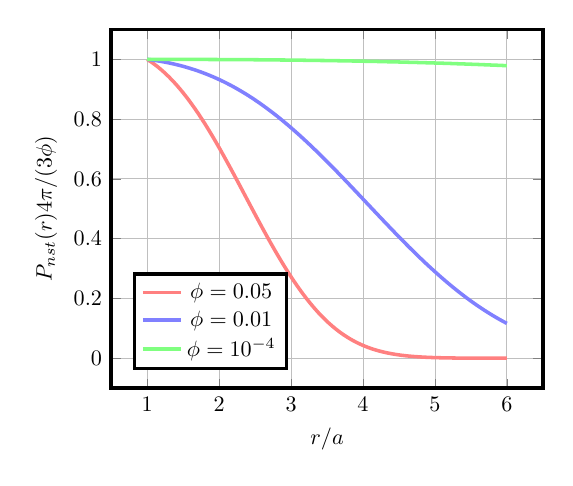
\begin{tikzpicture}[scale=0.8]
    \begin{axis}[
        xlabel={$r/a$},
        ylabel={$P_\text{nst}(r) 4\pi/ (3\phi) $},
        legend style={at={(0.05,0.05)}, anchor=south west},
        grid=major,
        domain=1:6,
        samples=100,
        ultra thick
    ]
    
    % Plot for phi = 0.05
    \addplot[color=red!50,ultra thick]
    { exp(-0.05 * (x^3 - 1))};
    \addlegendentry{$\phi = 0.05$}
    
    % Plot for phi = 0.01
    \addplot[color=blue!50,ultra thick]
    { exp(-0.01 * (x^3 - 1))};
    \addlegendentry{$\phi = 0.01$}
    
    % Plot for phi = 0.001
    \addplot[color=green!50,ultra thick]
    { exp(-0.0001 * (x^3 - 1))};
    \addlegendentry{$\phi = 10^{-4}$}
    
    \end{axis}
\end{tikzpicture}
\hfil
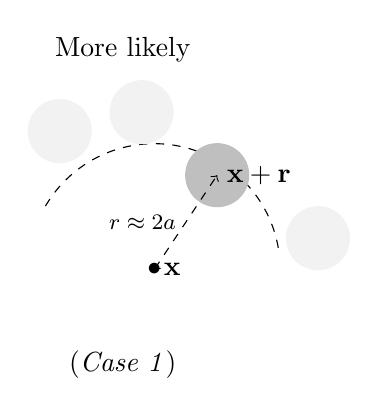
\begin{tikzpicture}[scale=0.8]
  \filldraw[ gray!10!white](+2.6,0.5)circle (0.5);
  \filldraw[ gray!10!white](-1.5,2.2)circle (0.5);
  \draw[dashed](10:2) arc (10:150:2);
  % \filldraw[ gray!50!white](0,0) circle (0.5);
  \filldraw[ gray!50!white](1,1.5)circle (0.5);
  \filldraw[ gray!10!white](-0.2,2.5)circle (0.5);
  \draw(0,0)node{$\bullet$}node[right]{$\textbf{x}$};
  \draw[dashed,<->](0,0)--(1,1.5)node[midway,left]{\footnotesize $r\approx 2 a$}node[right]{$\textbf{x}+\textbf{r}$};
  % \draw[dashed](-0.2,3.5);
  \node[ultra thick] (title) at (-0.5,3.5) {{More likely}};
  \node[ultra thick] (title) at (-0.5,-1.5) {(\textit{Case 1})};
\end{tikzpicture} 
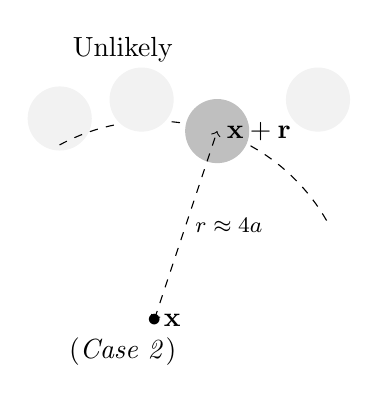
\begin{tikzpicture}[scale=0.8]
  \filldraw[ gray!10!white](+2.6,3.5)circle (0.5);
  \filldraw[ gray!10!white](-1.5,3.2)circle (0.5);
  \draw[dashed](30:3.16) arc (30:120:3.16);
  % \filldraw[ gray!50!white](0,0) circle (0.5);
  \filldraw[ gray!50!white](1,3)circle (0.5);
  \filldraw[ gray!10!white](-0.2,3.5)circle (0.5);
  \draw(0,0)node{$\bullet$}node[right]{$\textbf{x}$};
  \draw[dashed,<->](0,0)--(1,3)node[midway,right]{\footnotesize  $r\approx 4a$}node[right]{$\textbf{x}+\textbf{r}$};
  % \draw[dashed](-0.2,3.5);
  \node[ultra thick] (title) at (-0.5,4.3) {{Unlikely}};
  \node[ultra thick] (title) at (-0.5,-0.5) {(\textit{Case 2})};
\end{tikzpicture} 
\caption{(left) Plot of the normalized nearest neighbor distribution $P_\text{nst}$. 
(right) Sketches explaining the behavior of the nearest neighbor distribution $P_\text{nst}$: 
(\textit{Case 1}) A droplet located at $\textbf{x}+\textbf{r}$ relatively \underline{close} to a point occupied by the continuous phase at \textbf{x}; this situation is likely to happen. 
(\textit{Case 2}) A droplet located at $\textbf{x}+\textbf{r}$ relatively \underline{far} to a point occupied by the continuous phase at \textbf{x}; this situation very unlikely to happen.
Indeed, it implies that no particles are present within the sphere of radius $4a$ centered at $\textbf{x}$ since the nearest neighbor is located at a distance $4a$. 
}
\label{fig:P_nst_f}
\end{figure}
With these assumptions in place, we can compute the \textit{Reynolds stress} using, \ref{eq:relation_ensemble_nst} which reduces to the following formula, 
\begin{equation}
    \avg{\chi_f \textbf{u}_f'\textbf{u}_f'}/\phi_f
    = 
    \frac{3\phi}{4\pi}
    \int_{\mathbb{R}^6}
    \textbf{v}_f^\text{nst}
    \textbf{v}_f^\text{nst}
     e^{-\phi(r^3 -1)}
    d\textbf{r}
    d\textbf{w},
    \label{eq:step_one}
\end{equation}
where it must be understood that $\textbf{v}_f^\text{nst}$ is given by \ref{eq:stokes_sol}. 


Before computing the integration for Stokes flows, we would like to apply this formulation to re-compute the \textit{Reynolds stress} for translating spherical particles in potential flows. 
This will allow us to verify the consistency of our methodology. 
Indeed, it can be shown that \ref{eq:solution_isolated_at_x} also holds for the \textit{nearest neighbor conditionally averaged} momentum equations in potential flows, thus in that case $\textbf{v}^\text{nst}_f \approx \textbf{u}_f^{1d}$ where we recall that $ \textbf{u}_f^{1d}$ is given by \ref{eq:potential_sol}.
Therefore, we carry out the direct integration of \ref{eq:step_one} using \ref{eq:potential_sol} and obtain, 
\begin{equation}
    \avg{\chi_f \textbf{u}_f'\textbf{u}_f'}
    = \Gamma_\text{inc}(-1,\phi)\phi^2 e^\phi \left\{
        \frac{1}{20}[\textbf{u}_{fp}\textbf{u}_{fp}+ \frac{1}{n_p}\pavg{\textbf{u}_\alpha'\textbf{u}_\alpha'}]
        + 
        \frac{3}{20} (\textbf{u}_{fp}\cdot \textbf{u}_{fp} + 2k_p)\bm\delta
    \right\},
    \label{eq:potential_nst}
\end{equation}
where $\Gamma_\text{inc}$ is the gamma incomplete function. 
According to \ref{eq:potential_nst} our results differ with \ref{eq:van_wingarden_sol} by a factor of $\Gamma_\text{inc}(-1,\phi)\phi^2 e^\phi$. 
Nevertheless, this inconsistency is easily solved noticing that $\Gamma_\text{inc}(-1,\phi)\phi^2 e^\phi \sim \phi + \mathcal{O}(\phi^2)$. 
Thus, we conclude that at the leading order, our methodology seem consistent with the classical conditional average methodology introduced by \citet{batchelor1972sedimentation}. 

Now that we have all the tools in hand, let us carry out the direct integration of \ref{eq:step_one} for the wake of a spherical droplet in stokes flows. 
Using \ref{eq:solution_isolated_at_x} and \ref{eq:Pnst_explicit} in \ref{eq:step_one} gives, in dimensionless form,  
\begin{equation}
    \avg{\chi_f  \textbf{u}_f'\textbf{u}_f'}
    = 
    C_1
    \left\{
        \textbf{u}_{fp}\textbf{u}_{fp}+ \frac{1}{n_p}\pavg{\textbf{u}_\alpha'\textbf{u}_\alpha'}
        -\frac{1}{3} (\textbf{u}_{fp}\cdot \textbf{u}_{fp} + 2k_p)\bm\delta
    \right\},    
    +  C_2
    (\textbf{u}_{fp}\cdot \textbf{u}_{fp} + 2k_p)\bm\delta,
    \label{eq:final_closure}
\end{equation}
with,
\begin{align*}
    C_1(\phi,\lambda)
    = \frac{9(2+3\lambda)^2}{80(1+l)^2}
    % \left[
        \Gamma(1/3) \phi^{2/3}
        % - (27+82\lambda +62\lambda^2)
    % \right]
    ,
    &&
    C_2(\phi,\lambda)
    = \frac{(2+3\lambda)^2}{24(1+l)^2}
    % \left[
        \Gamma(1/3) \phi^{2/3}.
        % - (3+10\lambda +8\lambda^2)
    % \right].
\end{align*}
% \tb{maybe remove order phi terms}
We have decomposed the \textit{Reynolds stress} tensor into two contributions. 
The first term on the right-hand side of \ref{eq:final_closure} is a traceless symmetric tensor, proportional to the functional $C_1$. 
The second term is the isotropic part of the \textit{Reynolds stress} tensor, which is proportional to $C_2$. 

Additionally, we can note that, according to the value of $C_1$ and $C_2$, the \textit{pseudo turbulence} or \textit{Reynolds stress} induced by the translation of the droplets is higher for large values of $\lambda$. 
In other words, a solid particle in translation induces more velocity fluctuation than a bubble of the same size. 

Moreover, as witnessed by the presence of the term $\phi^{2/3}$, in $C_1$ and $C_2$, we conclude that the solution obtained here is still consistent with the observation made in \ref{eq:real_error} or in the previous study \citep{caflisch1985variance}. 
Indeed, for an isolated droplet, i.e. when we take the limit, $\phi \to 0$, we obtain $\lim_{\phi \to 0} \avg{\chi_f \textbf{u}_f' \textbf{u}_f'} / \phi = \infty$. 
Consequently, in agreement with the previous statements, the normalized \textit{Reynolds stress}, i.e. the Reynolds stress divided by the number density or $\phi$,  is infinite for an isolated droplet.
However, when considering a small but finite value of $\phi$ the \textit{Reynolds stress} remains finite and is given by \ref{eq:final_closure}. 

Finally, as it is not the \textit{Reynolds stress} divided by $\phi$ that matter, but $\avg{\chi_f\textbf{u}_f'\textbf{u}_f'}$ itself, note that at the leading order in $\phi$ we obtain,  $\avg{\chi_f\textbf{u}_f'\textbf{u}_f'}\sim\phi^{2/3}$. 
Notably, this trend in $\sim\phi^{2/3}$ is not new and agrees with previous studies found in the literature.
Specifically, in \citet{hill2001first} they compute \textit{Reynolds stress} for ordered array of solid spheres and found $k_f \sim 0.969 \phi^{2/3}$. 
\ref{eq:final_closure} with $\lambda =\infty$ gives, $k_f  = 1.50 \phi^{2/3}$.
The difference between our results and \citet{hill2001first}'s result, probably comes from the different particles arrangement considered.  



\subsection{Solution including the buoyancy force. }

Although we chose to neglect the source term in \ref{eq:momentum_nst_d_stokes} how can we be certain that it was indeed negligible? 
Even though this term is $\mathcal{O}(\phi)$ in $\textbf{v}^\text{nst}$, it does not necessarily imply that it will contribute at $\mathcal{O}(\phi)$ in $\avg{\rho_f\chi_f \textbf{u}_f'\textbf{u}_f'}$. 
Indeed, in \citet{zhang2021ensemble}, while carrying similar derivations, he found out that the terms of $\mathcal{O}(\phi)$ in the equation for $\textbf{v}^\text{nst}$, contributed to $\mathcal{O}(\phi^{1/3})$ in their final results.  
Thus, in this section we carry out the same calculation, but with the consideration of the buoyancy source term. 

\subsubsection{The velocity fields singularity solution}

Since the velocity field $\textbf{v}^\text{nst}$ still satisfy the linear Stokes equations, we may proceed into two steps. 

First, regardless of the right-hand side of \ref{eq:momentum_nst_d_stokes} the boundary condition at the surface of the particle, located at \textbf{y}, will generate the velocity fields \citep{pozrikidis1992boundary}, 
\begin{equation}
    \textbf{v}^\text{nst}[\textbf{z},t|\textbf{x},\textbf{w},\textbf{y}]
    = 
    % \frac{a}{4}(\textbf{w}- \textbf{u}[\textbf{y},t])\cdot\left[
    %     \frac{2+3\lambda}{1+\lambda}
    %     +
    %     a^2\frac{\lambda}{2(1+\lambda)}\pddz^2 
    % \right]\mathcal{G}(\textbf{z},\textbf{y}).
    \mathcal{U}[(\textbf{z} - \textbf{y})/a]\cdot 
    (\textbf{w}- \textbf{u}[\textbf{y},t]).
    \label{eq:solution_isolated2}
\end{equation}
Recall that $\mathcal{U}$ takes a dimensionless distance as argument. 

Secondly, let us turn our attention to the source term on the right-hand side of \ref{eq:momentum_nst_d_stokes}. 
Following \citet{zhang2021ensemble}, we remark that the contribution to the velocity field, generated by the particle-free zone, can be written as a sum of \textit{Stokeslets} of magnitude $\phi\Delta \rho \textbf{g}$.
Indeed, since the Dirac delta function is a unit of convolution product, we may write, 
\begin{equation}
    \phi \Delta\rho  \textbf{g} H(|\textbf{y} - \textbf{x}| - |\textbf{z} - \textbf{x}|)
    = 
    \phi \Delta\rho  \textbf{g} 
    \int_{|\textbf{y} - \textbf{x}| > |\textbf{x}' - \textbf{x}|}
    \delta(\textbf{x}'-\textbf{z})
    d\textbf{x}'. 
\end{equation}
Additionally, the velocity field evaluated at \textbf{z}, generated by the point force,  $\phi\Delta \rho \textbf{g}\delta(\textbf{x}' - \textbf{z})$, can be written \citep{pozrikidis1992boundary}, 
\begin{equation}
    \frac{\phi\Delta \rho \textbf{g}}{8\pi \mu_f}\cdot \mathcal{G}(\textbf{z} - \textbf{x}')
\end{equation}
where $\mathcal{G}(\textbf{r})$ is the Green function of the Stokes equations, namely, 
\begin{equation}
    \mathcal{G}(\textbf{r}) = \frac{\bm\delta}{r} + \frac{\textbf{rr}}{r^3}.
\end{equation}
Consequently, the velocity fields generated by the right-hand-side of \ref{eq:momentum_nst_d_stokes}, meaning by particle-free zone, as given in \ref{fig:unst}, can be written as, 
\begin{equation}
    \textbf{v}_b^\text{nst}[\textbf{z},t|\textbf{y},\textbf{w},\textbf{x}]
    = 
    \frac{\phi\Delta \rho \textbf{g}}{8\pi \mu_f}\cdot 
    \int_{|\textbf{x}'-\textbf{x}|< |\textbf{y}- \textbf{x}|}
    \mathcal{G}(\textbf{z} - \textbf{x}')
    d\textbf{x}'
    \label{eq:v_b_sol}
\end{equation}
where we used the subscript $_b$ to denote the particle-free zone contribution. 
Due to the linearity of the Stokes equations, the total velocity field is thus the sum of \ref{eq:solution_isolated2} and \ref{eq:v_b_sol}. 
% Likewise, the stress generated by the particle-free-zone might be written \citep{pozrikidis1992boundary},
% \begin{equation}
%     \bm\sigma_b^\text{nst}[\textbf{z},t|\textbf{y},\textbf{w},\textbf{x}]
%     = 
%     \frac{\phi\Delta \rho \textbf{g}}{8\pi}\cdot 
%     \int_{|\textbf{x}'-\textbf{x}|< |\textbf{y}- \textbf{x}|}
%     \mathcal{T}(\textbf{z},\textbf{x}')
%     d\textbf{x}'
%     \label{eq:sigma_b_sol}
% \end{equation}
% with, 
% \begin{equation}
%     \mathcal{T}(\textbf{z},\textbf{x}')
%     = - 6\frac{\textbf{rrr}}{r^5}. 
% \end{equation}
% Here, $\textbf{r} = \textbf{z} - \textbf{x}'$. 

Therefore, the total velocity field $\textbf{v}^\text{nst}_f$ at the point $\textbf{x}$, can be obtained using \ref{eq:v_b_sol} and \ref{eq:solution_isolated2} evaluated at the point \textbf{x}, and  \ref{eq:reformulation}, which yields,  
\begin{multline}
    \textbf{v}^\text{nst}_f [\textbf{x},\textbf{w},\textbf{y},t]
    =
    % \frac{a}{4}(\textbf{w}- \textbf{u}[\textbf{y},t])\cdot\left[
    %     \frac{2+3\lambda}{1+\lambda}
    %     +
    %     a^2\frac{\lambda}{2(1+\lambda)}\grad^2 
    % \right]\mathcal{G}(\textbf{x},\textbf{y})
    \mathcal{U}[(\textbf{x} - \textbf{y})/a]\cdot 
    (\textbf{w}- \textbf{u}[\textbf{y},t])
    \\
    +
    \phi(\textbf{u}_d - \textbf{u}_f)
    + 
    \frac{\phi\Delta \rho \textbf{g}}{8\pi \mu_f}\cdot 
    \int_{|\textbf{x}'-\textbf{x}|< |\textbf{y}- \textbf{x}|}
    \mathcal{G}(\textbf{x},\textbf{x}')
    d\textbf{x}',
\end{multline}
Carrying out the integral on the second line directly gives,
\begin{equation}
    \int_{|\textbf{x}'-\textbf{x}|< |\textbf{y}- \textbf{x}|}
    \mathcal{G}(\textbf{x},\textbf{x}')
    d\textbf{x}'
    = \frac{8\pi}{3}|\textbf{x}- \textbf{y}|^2\bm\delta
\end{equation}
Note that using a similar procedure one can evaluate the contribution to the velocity field of the $\textbf{S}_p^{(2)}$ however it turns out to be exactly zero.
\footnote{
    The ensemble averaged second moment of forces have the form $\textbf{S}_p^{(2)} \sim \phi \mu_f \textbf{u}_{pf} \bm\delta$. 
    Thus, the contribution of this term in \ref{eq:momentum_nst_d_stokes} is of the form, 
    \begin{equation*}
        \phi \mu_f \textbf{u}_{pf} \grad^2  H(|\textbf{y}- \textbf{x}| - |\textbf{z} -\textbf{x}|)
        =  \phi \mu_f \textbf{u}_{pf} \grad\grad \int_{|\textbf{y} - \textbf{x}| > |\textbf{x}' - \textbf{x}|}
        \delta(\textbf{x}'-\textbf{z})
        d\textbf{x}',
    \end{equation*}
    if one assume that the mean slip velocity $\textbf{u}_{pf}$ as well as the volume fraction $\phi$ is not a function of \textbf{z}. 
    Consequently, the velocity fields generated by this contribution can be written as, 
    \begin{equation*}
        \phi \mu_f \textbf{u}_{pf} \grad^2  H(|\textbf{y}- \textbf{x}| - |\textbf{z} -\textbf{x}|)
        \rightarrow \phi \mu_f \textbf{u}_{pf} \int_{|\textbf{y} - \textbf{x}| > |\textbf{x}' - \textbf{x}|}
        \grad\grad\mathcal{G}(\textbf{z} - \textbf{x}')
        d\textbf{x}'. 
    \end{equation*}     
    Evaluating this expression at $\textbf{z} = \textbf{x}$ gives, 
    \begin{equation*}
        \phi \mu_f \textbf{u}_{pf} \int_{|\textbf{y} - \textbf{x}| > |\textbf{r}|}
        \grad^2\mathcal{G}(\textbf{r})
        d\textbf{r} 
        = 
        \phi \mu_f \textbf{u}_{pf} \int_{|\textbf{y} - \textbf{x}| > |\textbf{r}|}
        (\frac{\bm\delta}{r^3} - \frac{3\textbf{rr}}{r^5})
        d\textbf{r} 
        = 0. 
    \end{equation*}     
    Hence, contributing to nothing in $\textbf{v}_f^\text{nst}$.
} 
It finally gives the result, 
\begin{equation}
    \textbf{v}^\text{nst}_f
    =
    \mathcal{U}[(\textbf{x} - \textbf{y})/a]\cdot 
    (\textbf{w}- \textbf{u}_f[\textbf{y},t])
    + 
    \frac{\Delta \rho \textbf{g}a^2}{3\mu_f} \frac{ |\textbf{x}-\textbf{y}|^2}{a^2}\phi
    +
    \mathcal{O}(\phi).
    \label{eq:final_sol_v_nst}
\end{equation}
Note that we neglected the $\mathcal{O}(\phi)$ terms however we must keep the buoyancy term as it is of $\mathcal{O}(|\textbf{x}-\textbf{y}|^2/a^2\phi)$ which remains significant  for large $|\textbf{x}-\textbf{y}|/a$, or more precisely for the distances such that $|\textbf{x}-\textbf{y}|/a  > 1/\sqrt{\phi}$. 
In this expression, we clearly identify $2$ distinct contributions. 
The first two terms on the right-hand side of \ref{eq:final_sol_v_nst} correspond to the disturbance field generated by an isolated droplet, which was the only contribution in \ref{eq:solution_isolated_at_x}. 
The third term corresponds to the ``backflow velocity'' as called by \citet{zhang2021ensemble}, it refers to the flow generated by the particle-free zone, due to buoyancy forces. 
% Finally, the last term ensure that we stay in the right reference frame. 
Note that in \citet[Appendix A]{zhang2021ensemble} they carried out nearly the same calculation for solid particles.
One can note a small differences between \ref{eq:final_sol_v_nst} with $\lambda = \infty$ and Eq. (B 4) of  \citet[Appendix A]{zhang2021ensemble} , indeed, while $(\textbf{w}- \textbf{u}_f[\textbf{y},t])$ is in factor of the first term in \ref{eq:final_sol_v_nst}, \citet[Appendix A]{zhang2021ensemble} obtained the factor $(\textbf{w}- \textbf{u}_f - \textbf{v}_b^\text{nst})$. 
This is due to the different reference frames used for the velocity fields.
Indeed, here we solved for $\textbf{v}^\text{nst}$ while in \citet{zhang2021ensemble} they solve for $\textbf{u}^\text{nst}$. 
The consequence is that, while we have only one source term at the right-hand side of \ref{eq:momentum_nst_d_stokes}, \citet{zhang2021ensemble} has a supplementary, constant source term overall the domain. 
This is the reason for the presence of his $\textbf{v}_b'$ which is not present in \ref{eq:final_sol_v_nst}. 
% Thus, our result is consistent with \citet{zhang2021ensemble}, moreover, we generalized and demonstrated his results for spherical droplets. 


For a better physical understanding, we present now the dimensionless form of \ref{eq:final_sol_v_nst}. 
The lengths are made dimensionless using the radius of the particle $a$ such that $\textbf{r} = |\textbf{x} - \textbf{y}|/a$, the velocity vector $\textbf{w} - \textbf{u}_f$ is made dimensionless using $U = |\textbf{w} - \textbf{u}_f|$, 
We also introduce the unit vector: $\textbf{e} = (\textbf{w} - \textbf{u}_f)/U$. 
Likewise, the gravity acceleration vector is made dimensionless using its norm, such that the unit vector in the direction of the acceleration of gravity is given by $\textbf{k} = \textbf{g} / g$, with $g = |\textbf{g}|$. 
Dividing \ref{eq:final_sol_v_nst} by $U$ and using these definitions yields directly the dimensionless expression for the disturbance velocity field, 
\begin{equation}
    \frac{\textbf{v}^\text{nst}_f}{U}
    =
    \mathcal{U}(\textbf{r})\cdot 
    \textbf{e}
    + \phi A |\textbf{r}|^2 \textbf{k}
    + \mathcal{O}(\phi). 
    \label{eq:v_nst_solution_adim}
\end{equation}
Where we introduced the dimensionless number, 
\begin{equation}
    A = \frac{Ga^2}{12 Re}=\frac{\Delta \rho g (2a)^2}{12 \mu_f U}
    \label{eq:A_general}
\end{equation}
where we recall that $Ga$ is the \textit{Galileo} number and $Re$ the \textit{Reynolds} number, defined as,  
\begin{align*}
    Re= \frac{\rho_f U 2a}{\mu_f},
    &&
    Ga^2 = \frac{\rho_f \Delta\rho g (2a)^3}{\mu_f^2},
\end{align*}
respectively. 
Upon considering specific scenarios, such as a steady state buoyant rising droplet, one is able to relate $Ga$ and $Re$ and give an explicit expression for the term $A$.
 



\subsubsection{The pseudo turbulent tensor closure}

From \ref{eq:v_nst_solution_adim} we may already compute the integral in \ref{eq:step_one}. 
However, as $\textbf{e}$ and $\textbf{k}$ in \ref{eq:v_nst_solution_adim}  are not necessarily collinear vectors, the functional form of the resulting stress tensor is not trivial. 
Indeed, since $\textbf{v}_f^\text{nst}\sim \textbf{e}$ and $\sim \textbf{k}$, the final results must be a tensor built from sums of products of these two vectors.  
Additionally, since $\avg{\rho_f \textbf{u}_f'\textbf{u}_f'}$ is a symmetric tensor, the result must be a symmetric tensor as well. 
The only second-order symmetric tensors that can be constructed from the  two arbitrary vectors: $\textbf{e}$ and $\textbf{k}$ are, 
\begin{align*}
    \textbf{ee}
    && (\textbf{e}\cdot \textbf{e})\bm\delta, 
    && \textbf{kk},
    && (\textbf{k}\cdot \textbf{k})\bm\delta,
    && \textbf{ke}+\textbf{ek},
    && (\textbf{k}\cdot \textbf{e})\bm\delta, 
\end{align*}
we deduce that the volume integral of \ref{eq:step_one}, reads, 
\begin{align}
    \frac{1}{U^2}
    \frac{3\phi}{4\pi}\int_{\mathbb{R}^3}
    \textbf{v}_f^\text{nst}
    \textbf{v}_f^\text{nst}
     e^{-\phi(r^3 -1)}
    d\textbf{r}
    &= C^{(1)}_e \left[
        \textbf{ee}
         - \frac{1}{3}(\textbf{e}\cdot \textbf{e})\bm\delta
    \right]
    + C^{(2)}_e 
    (\textbf{e}\cdot \textbf{e})\bm\delta \nonumber \\
    &+ C^{(1)}_k \left[
        \textbf{kk}
         - \frac{1}{3}(\textbf{k}\cdot \textbf{k})\bm\delta
    \right]
    + C^{(2)}_k 
    (\textbf{k}\cdot \textbf{k})\bm\delta \nonumber \\
    &+ C^{(1)}_{ek} \frac{1}{2}\left[
        (\textbf{ek}  + \textbf{ke})
         - \frac{2}{3}(\textbf{k}\cdot \textbf{e})\bm\delta
    \right]
    + C^{(2)}_{ek} 
    (\textbf{e}\cdot \textbf{k})\bm\delta 
    \label{eq:functional_form}
\end{align}
where the first term of each line correspond to symmetric traceless tensors, and the second term of each line to the corresponding isotropic contribution. 
The first two constant, $C^{(1)}_e$ and $C^{(2)}_e$ can be obtained setting $\textbf{k}= 0$ in \ref{eq:v_nst_solution_adim} and performing the integration. 
Likewise, $C^{(1)}_k$ and $C^{(2)}_k$ can be obtained setting $\textbf{e}=0$ in \ref{eq:v_nst_solution_adim}. 
The constants, $C^{(1)}_{ek}$ and $C^{(2)}_{ek}$ can be obtained setting $\textbf{g} = 0$ in of the $\textbf{v}_f^\text{nst}$ on the left-hand side of \ref{eq:functional_form} and $\textbf{e}=0$ in the other $\textbf{v}_f^\text{nst}$. 
Thus, we obtain at the leading order, 
\begin{align}
    C_e^{(1)} =
    % \frac{9(2+3\lambda)^2 \Gamma(\frac{1}{3})}{80(\lambda+1)^2}\phi^{2/3}
    \frac{27}{10}
    C_e^{(2)}
    % + \mathcal{O}(\phi)
    &&  C_e^{(2)} =
    \frac{(2+3\lambda)^2 \Gamma(\frac{1}{3})}{24(\lambda+1)^2}\phi^{2/3}
    + \mathcal{O}(\phi)
    \\
    C_k^{(1)} =
    % A^2 \Gamma\left(7/3\right)\phi^{2/3}
    3
    C_k^{(2)}
    % + \mathcal{O}(\phi^{5/3})
    && C_k^{(2)} =
    A^2 \frac{\Gamma(\frac{7}{3})}{3}\phi^{2/3}
    + \mathcal{O}(\phi^{5/3})
    \\
    C_{ek}^{(1)} =
    3
    C_{ek}^{(2)}
    % A\frac{2 (2+3\lambda) \Gamma(\frac{4}{3})}{3 (\lambda+1)}\phi^{2/3}
    % + \mathcal{O}(\phi^{4/3})
    && C_{ek}^{(2)} =
    A\frac{2 (2+3\lambda) \Gamma(\frac{4}{3})}{9(\lambda+1)}\phi^{2/3}
    + \mathcal{O}(\phi^{4/3})
    \label{eq:constants}
\end{align}
Note that $C_e^{(1)}$ and $C_e^{(2)}$ correspond to the constants obtained in \ref{eq:final_closure}. 
Additionally, note that the leading order contribution from the backflow velocity is $\sim \phi^{2/3}$ as well. 
Therefore, these new terms are non-negligible in this general framework. 


Following \ref{eq:step_one}, to obtain the ensemble-averaged \textit{Reynolds stress} tensor we now integrate  \ref{eq:functional_form} over all the $\textbf{w}$.
This yields the final form of the \textit{Pseudo turbulent} tensor, which reads 
\begin{align}
    \frac{\avg{\chi_f \textbf{u}_f'\textbf{u}_f'}}{\phi_f U^2}
    &= 
    C^{(1)}_e \left[
        \textbf{e}_p\textbf{e}_p
        + \frac{\pavg{\textbf{u}_\alpha'\textbf{u}_\alpha'}}{n_p U^2}
         - \frac{1}{3}(\textbf{e}_p\cdot \textbf{e}_p+2k_p/U^2)\bm\delta
    \right]
    + C^{(2)}_e 
    (\textbf{e}_p\cdot \textbf{e}_p+2k_p/U^2)\bm\delta \nonumber \\
    &+ C^{(1)}_k  \left[
        \textbf{kk}
         - \frac{1}{3}(\textbf{k}\cdot \textbf{k})\bm\delta
    \right]
    +C^{(2)}_k 
    (\textbf{k}\cdot \textbf{k})\bm\delta \nonumber \\
    &+ C^{(1)}_{ek} \left[
        \frac{1}{2}
        (\textbf{e}_p\textbf{k}  + \textbf{k} \textbf{e}_p)
         - \frac{1}{3}(\textbf{k}\cdot \textbf{e}_p)\bm\delta
    \right]
    + C^{(2)}_{ek}
    (\textbf{e}_p\cdot \textbf{k})\bm\delta. 
    \label{eq:functional_form_avg}
\end{align}
In this expression $\textbf{e}_p = \int \textbf{e} d\textbf{w} $ represents the mean direction of the mean relative phase velocity $\textbf{u}_{pf}$ such that $\textbf{u}_{pf} = U \textbf{e}_p$, in opposition to $\textbf{e}$ which represented the direction of a single particle relative velocity. 



In summary, the only additional terms appearing due to the integration over the velocity phase space is the addition of the particle fluctuation contribution to the \textit{Reynolds stress}. 
However, it is likely that $k_p/U^2 \sim \phi^{2/3}$ as suggested by experimental results reported in \citet{guazzelli2011fluctuations} and theoretical investigation of \citet{caflisch1985variance}.
Therefore, this term end up adding a contribution of $\mathcal{O}(\phi^{4/3})$ in $\avg{\chi_f \textbf{u}_f'\textbf{u}_f'}$, hence it can be neglected at $\mathcal{O}(\phi)$. 



\subsubsection{Steady-state rising droplet}

Let us now study the case where $\textbf{k} = - \textbf{e} = \textbf{e}_z$, meaning that the droplet rises in the opposite direction of gravity which is acting in the vertical direction denoted by $\textbf{e}_z$.  
At $\mathcal{O}(\phi)$ and in Stokes flow regime, the drag applied on a spherical droplet is given by the formula of Hadamard-Ribczynski.
Thus, the magnitude of the steady-state rising velocity of a droplet is given by, 
\begin{equation}
    U = \Delta \rho \frac{2 g a^2}{3 \mu_f }\left(\frac{1+\lambda}{2+3\lambda}\right).
    \label{eq:U_isolated}
\end{equation}
% \begin{equation}
%     2a \pi \mu_f \left(\frac{3\lambda +2}{\lambda +1}\right) 
%     U
%     = 
%     \frac{4}{3}\pi a^3 
%     \Delta \rho
%     g,
% \end{equation}
We deduce from this relation that in this specific situation, i.e. when the direction of the relative velocity \textbf{e} is aligned with the gravity acceleration direction, we have, 
\begin{equation}
    A = \frac{1}{2}\left(\frac{3\lambda +2}{\lambda +1}\right). 
    \label{eq:closure_A}
\end{equation}
Injecting this expression into \ref{eq:v_nst_solution_adim} gives us an explicit expression of the velocity field $\textbf{v}^\text{nst}_f$. 

To give a better idea of the meaning of $\textbf{v}_f^\text{nst}$, we display 
in \ref{fig:vnst_vertical} the streamlines generated by the field $\textbf{v}_f^\text{nst}(\textbf{r})$ in the cross-section, given by the plane formed by the vectors $(\textbf{e}_x,\textbf{e}_z)$, although the velocity field is axisymmetric. 
\begin{figure}[h!]
    \centering
    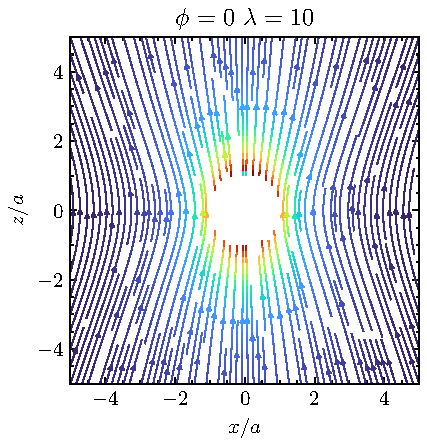
\includegraphics[height = 0.33\textwidth]{image/Vnst_l_10_0.pdf}
    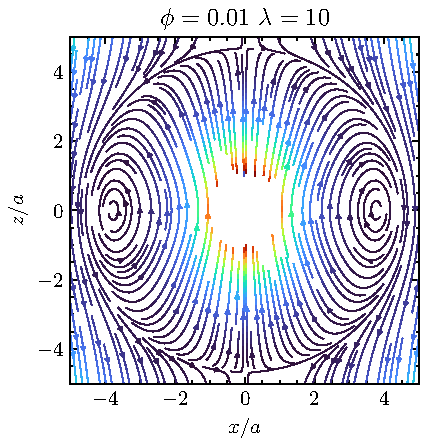
\includegraphics[height = 0.33\textwidth]{image/Vnst_l_10_1.pdf}
    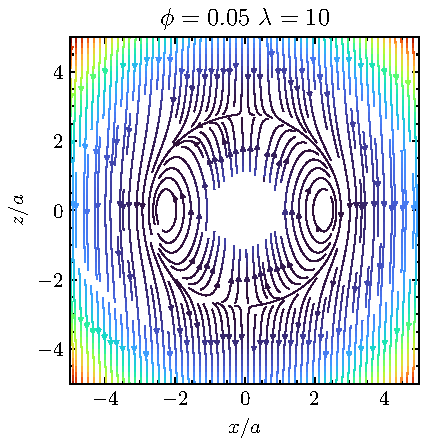
\includegraphics[height = 0.33\textwidth]{image/Vnst_l_10_5.pdf}
    % 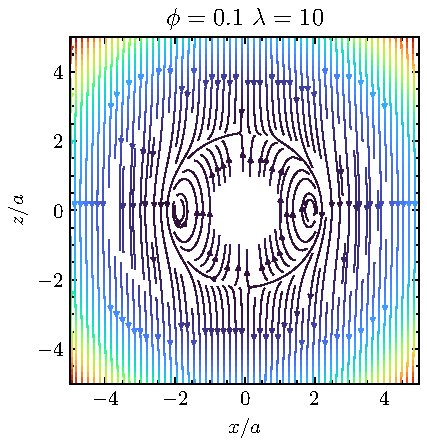
\includegraphics[height = 0.33\textwidth]{image/Vnst_l_10_10.pdf}
    \caption{Streamlines of the disturbance velocity field $\textbf{v}_f^\text{nst}(\textbf{r}_f)$ \eqref{eq:v_nst_solution_adim}  in the cross-section given by the plane $(\textbf{e}_x,\textbf{e}_z)$, for multiples volume fraction $\phi = 0, 0.01$ and $0.05$ at $\lambda = 10$.  
    The color map indicates the magnitude of the velocity, from black which corresponds to a velocity magnitude of 0, to the color at the interface which corresponds to 1.
    In this situation $\textbf{e} = \textbf{e}_z$ and $\textbf{k} = -\textbf{e}_z$}
    \label{fig:vnst_vertical}
\end{figure}
We can observe on \ref{fig:vnst_vertical} (left) that $\textbf{v}^\text{nst}_f(\phi =0)$ corresponds to the disturbance field of an isolated particle in Stokes flow. 
This is easily understandable considering that the last term on the right-hand side of \ref{eq:v_nst_solution_adim} cancel for $\phi=0$, thus leaving us with an expression equivalent to \ref{eq:solution_isolated}, which is the disturbance field of an isolated particle. 
At finite volume fraction, $\phi =0.01$, we  observe in \ref{fig:vnst_vertical} (middle), that a downstream velocity starts to appear at a large distance from the particle center.  
As discussed previously, this ``backflow velocity'' is given by the term $\phi A |\textbf{x}- \textbf{y}|^2 \textbf{k}$ in \ref{eq:solution_isolated}.
The particle is thus surrounded by a spherical shell within which the disturbance field has a positive vertical velocity, and outside which the velocity is negative.
In the following discussion, we call this spherical shell the \textit{recirculation region}.   
For higher volume fractions ($\phi = 0.05$), the backflow velocity is even stronger leading to a smaller recirculation region around the particle. 

Let us discuss the form of \ref{eq:functional_form_avg} in the specific case displayed in \ref{fig:vnst_vertical}, i.e. spherical droplets rising in stokes flow. 
Since $\textbf{e}_p = - \textbf{k}$ we have $\textbf{e}_p\textbf{k} = - \textbf{kk}$. 
Additionally, one can use \ref{eq:closure_A} into the expression for $C_k^{(1)}$ and $C_{ek}^{(1)}$. 
In this specific case, by carrying out the calculation, we obtain, 
\begin{equation}
    C_k^{(1)} \textbf{kk} + C_{ek}^{(1)} \textbf{ke}_p
    = 0. 
    \label{eq:cancelation1}
\end{equation}
Applying the same reasoning, one can also deduce that, 
\begin{equation}
    C_k^{(2)} \textbf{k}\cdot \textbf{k} + C_{ek}^{(2)} \textbf{k}\cdot \textbf{e}_p
    = 0. 
    \label{eq:cancelation2}
\end{equation}
Consequently, we deduce that the contribution from the gravity acceleration to the \textit{Reynolds stress} tensor, remains zero in this simplified situation. 
This might seem surprising considering the seemingly non-negligible action of the gravity on the velocity field displayed \ref{fig:vnst_vertical}. 
However, we must understand from this, that the velocity variance generated by the backflow velocity, also induces a decrease of the velocity variance generated by the particle motion compared to the isolated case.
In other words, the backflow velocity generated at the boundaries of the recirculation region has a low-velocity variance, which is exactly balanced by the velocity variance generated by the backflow at the exterior of the recirculation region.    
Note that this explanation is only true when $\textbf{k} = - \textbf{e}_p$. 

In the next section we examine a situation where the velocity of the dispersed phase is not in the opposite direction of gravity. 



\subsubsection{Horizontal motions}

We now consider the case were $\textbf{e}_p = \textbf{e}_x$, and $\textbf{k} = - \textbf{e}_z$, where $\textbf{e}_z$ is still the vertical unit vector and $\textbf{e}_x$ the Horizontal unit vector. 
Of course, in the steady-state regime and isolated from the boundary of the domain, $\textbf{e}_p$, cannot be otherwise than vertical.  
However, in a more general case, $\textbf{e}_p$ have absolutely no reason to be in the vertical direction due inertial effects.
Hence, studying this situation remains relevant, as it represents the zeroth-order term of an inertial solution expanded in a Taylor series with respect to $Re$.  
In this case, $A$ is given by \ref{eq:A_general} and requires the norm of the relative velocity $U$ to be computed.

\begin{figure}[h!]
    \centering
    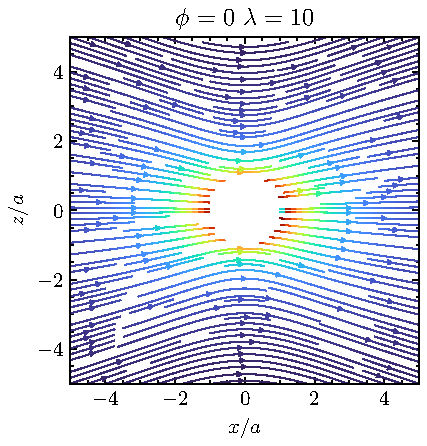
\includegraphics[height = 0.33\textwidth]{image/Vnst_H_l_10_0.pdf}
    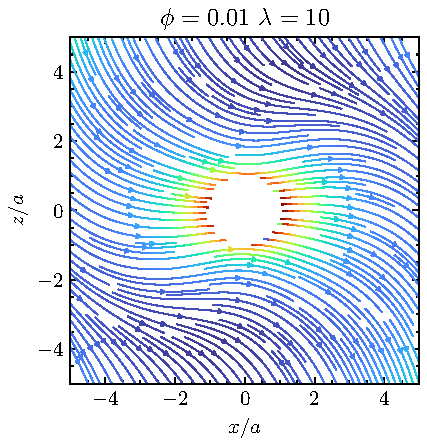
\includegraphics[height = 0.33\textwidth]{image/Vnst_H_l_10_1.pdf}
    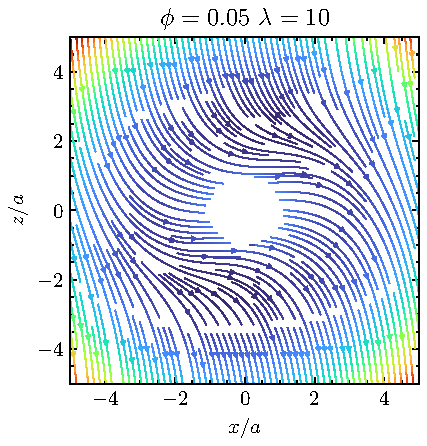
\includegraphics[height = 0.33\textwidth]{image/Vnst_H_l_10_5.pdf}
    % 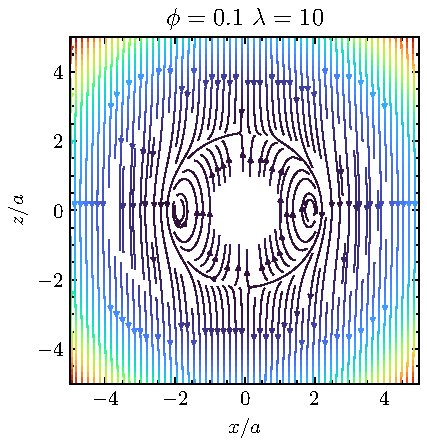
\includegraphics[height = 0.33\textwidth]{image/Vnst_l_10_10.pdf}
    \caption{Streamlines of the disturbance velocity field $\textbf{v}^\text{nst}(\textbf{r}_f)$  \eqref{eq:v_nst_solution_adim} in the cross-section given by the plane $(\textbf{e}_x,\textbf{e}_z)$, for multiples volume fraction $\phi = 0, 0.01$ and $0.05$ at $\lambda = 10$.  
    The color map indicates the magnitude of the velocity, from black which corresponds to a velocity magnitude of 0, to the color at the interface which corresponds to 1.
    In this situation $\textbf{e} = \textbf{e}_x$ and $\textbf{k} = -\textbf{e}_z$.
    The constant $A$ have been arbitrarily set to $1$. }
    \label{fig:vnst_horizontal}
\end{figure}
In \ref{fig:vnst_horizontal} we display the streamlines generated by the velocity field $\textbf{v}_f^\text{nst}$. 
As before, we remark that at $\phi = 0$, $\textbf{v}_f^\text{nst}$ corresponds to the disturbance velocity field of an isolated droplet translating horizontally in Stokes flow. 
At $\phi = 0.01$, see \ref{fig:vnst_horizontal} (middle), the effect of gravity induces a downstream backflow, this time, it is not in the opposite direction of the disturbance velocity of the drop.
At higher volume fractions this downstream flow is stronger, and the recirculation region around the particle is smaller. 
Note that at $|\textbf{r}|\to\infty $, $\textbf{v}^\text{nst}$ represents a vertical downstream flow. 
In short, we observe the same phenomenon as in the situation reported on \ref{fig:vnst_vertical}, except that the droplet disturbance field is not in the opposite direction of the backflow velocity. 

In this situation, the relation given by \ref{eq:cancelation1} and \ref{eq:cancelation2} are not valid anymore. 
Thus, in this case, the \textit{Reynolds stress} tensor is given by, 
\begin{equation}
    \frac{\avg{\chi_f \textbf{u}_f'\textbf{u}_f'}}{\phi_f U^2}
    = 
    C^{(1)}_e 
    \textbf{e}_x\textbf{e}_x
    % + \frac{\pavg{\textbf{u}_\alpha'\textbf{u}_\alpha'}}{n_p U^2}
    +C^{(1)}_k    
    \textbf{e}_z\textbf{e}_z
    - C^{(1)}_{ek} 
        \frac{1}{2}
        (\textbf{e}_x\textbf{e}_z+ \textbf{e}_z \textbf{e}_x)
    + [C^{(2)}_e + C^{(2)}_k - (C^{(1)}_k + C^{(1)}_e )/3 ]  \bm\delta. 
\end{equation}
The contribution from the wake of the particles is still present and is given by $C_e^{(1)}$ and $C_e^{(2)}$. 
This contribution is aligned with the direction of the droplet velocity, $\textbf{e}_x\textbf{e}_x$. 
Regarding the buoyancy forces, it provides an additional contribution that is proportional to $\textbf{e}_z\textbf{e}_z$. 
Finally, the cross terms $\textbf{e}_p \textbf{k}$ provide off-diagonal terms proportional to $\textbf{e}_z \textbf{e}_x$ or $\textbf{e}_x \textbf{e}_z$. 
The isotropic part of this tensor is the sum of the aforementioned contributions. 
Consequently, this proves that the Reynolds stress tensor posses off diagonal terms given by $C^{(1)}_{ek} 
\frac{1}{2} (\textbf{e}_x\textbf{e}_z+ \textbf{e}_z \textbf{e}_x)$ , that are related to the correlation of the backflow with the droplet disturbance field. 

\subsection{Discussion}

In this section, we have considered the translating motion of a spherical droplet in Stokes flow. 
The \textit{Reynolds stress} closure obtained is a function of $\textbf{u}_{fp}$ the relative phase velocity and the direction of the buoyancy force $\textbf{g}$. 
In the low inertia and dilute regime, we have shown that the ambient body force field $\textbf{g}$ plays a non-negligible role on the \textit{Nearest Neighbor Conditional Averaged} disturbance fields.
When the droplet translation is vertical (in the opposite direction of gravity) the terms related to the buoyancy force turn out to cancel out in the \textit{Reynolds stress} closure.
However, we have shown that it is not the case when the droplet's mean motion were not aligned with the direction of gravity.  

To extend this model, one must consider a more general ambient field, not only a uniform velocity field as demonstrated in this section, but mean shearing motions, or quadratic flows and so on. 
This will be the purpose of the last section of this chapter. 
Nevertheless, as this theoretical approach is new, we focus on numerically validating this model as a first step. 

% \section{Numerical experiments. }

In this section, we compare the theoretical results, to the numerical results obtained with \texttt{Basilisk} introduced in \ref{chap:DNS}. 
We recall that we are working with a set of simulations covering the parameter ranges displayed in \ref{tab:simulations_recall}. 
\begin{table}[h!]
    \centering
    \caption{Dimensionless parameter range investigated in this work.}
    \begin{tabular}{|ccccccc|ccc|}
        \hline
        \multicolumn{7}{|c}{Primary parameters} & \multicolumn{3}{||c|}{Secondary parameters}\\ \hline
        \multicolumn{1}{|c|}{$Ga$}                               & \multicolumn{1}{c|}{$Bo$}                   & \multicolumn{1}{c|}{$\phi$} & \multicolumn{1}{c|}{$\lambda$}                    & \multicolumn{1}{c|}{$\zeta$}                & \multicolumn{1}{c|}{$N_b$} & $t^*_\text{end}$ & \multicolumn{1}{||c|}{$\mathcal{L}/d$} & \multicolumn{1}{c|}{$Re$}  & $We$   \\ \hline
        \multicolumn{1}{|c|}{\multirow{4}{*}{$5\rightarrow 80$}} & \multicolumn{1}{c|}{\multirow{4}{*}{$0.5$}} & \multicolumn{1}{c|}{$1\%$}  & \multicolumn{1}{c|}{\multirow{4}{*}{$10$ \& $1$}} & \multicolumn{1}{c|}{\multirow{4}{*}{$0.9$}} & \multicolumn{1}{c|}{$160$} & $400$           & \multicolumn{1}{||c|}{$20$}            & \multicolumn{1}{c|}{$1.1\to 110$} & {$0.03\to 0.95$} \\ 
        \multicolumn{1}{|c|}{}                                   & \multicolumn{1}{c|}{}                       & \multicolumn{1}{c|}{$5\%$}  & \multicolumn{1}{c|}{}                             & \multicolumn{1}{c|}{}                       & \multicolumn{1}{c|}{$800$} & $400$           & \multicolumn{1}{||c|}{$20$}            & \multicolumn{1}{c|}{$0.8\to 92$} &  {$0.02\to 0.67$}\\ 
        \multicolumn{1}{|c|}{}                                   & \multicolumn{1}{c|}{}                       & \multicolumn{1}{c|}{$10\%$} & \multicolumn{1}{c|}{}                             & \multicolumn{1}{c|}{}                       & \multicolumn{1}{c|}{$200$} & $1000$           & \multicolumn{1}{||c|}{$10$}            & \multicolumn{1}{c|}{$0.64\to 77$}&  {$0.01\to 0.47$}\\ 
        \multicolumn{1}{|c|}{}                                   & \multicolumn{1}{c|}{}                       & \multicolumn{1}{c|}{$20\%$} & \multicolumn{1}{c|}{}                             & \multicolumn{1}{c|}{}                       & \multicolumn{1}{c|}{$400$} & $1000$           & \multicolumn{1}{||c|}{$10$}            & \multicolumn{1}{c|}{$0.43\to 62$}&  {$9\cdot 10^{-3}\to 0.31$}\\ \hline
        \end{tabular}
    \label{tab:simulations_recall}
\end{table}
In the first step, we will make use of the simulation results at $Ga = 5$ which is considered to be comparable to the Stokes regime used for the theory. 
However, note that at $Ga = 5$, $Re \approx 1$ consequently inertial effects are already present. 
Nevertheless, due to numerical constraints lower \textit{Reynolds} numbers could not be reached. 

The two main results that we are seeking to validate are, the disturbance fields expression \eqref{eq:v_nst_solution_adim} and the \textit{Reynolds} stress closure tensor, \eqref{eq:functional_form_avg}. 
Consequently, in the first part of this section, we focus on the comparison of $\textbf{v}_f^\text{nst}$ obtained with the DNS to the solution given by \ref{eq:v_nst_solution_adim}.
Then, we compare the numerical value of $\avg{\chi_f \textbf{u}_f'\textbf{u}_f'}$ with the prediction of \ref{eq:functional_form_avg}. 
Finally, our goal will be to extend \ref{eq:functional_form_avg} to non-negligible inertial effect and volume fraction effects, i.e. to higher $Re$ and $\phi$. 

\subsection{Nearest neighbors conditionally averaged disturbance velocity}

To reconstruct $\textbf{v}_f^\text{nst}$ with the DNS we must discretize \ref{eq:def_f_nst}. 
We proceed as follows: 
(1) We consider all simulations time steps and locations in the mesh as an independent configuration $\FF$.
This assumption holds since the system is homogeneous and statistically steady in time.  
Thus, we consider that the field $\textbf{u}_f^0[\textbf{x},\FF,t]$ is given by the field $\textbf{u}[c,t]$, where $c$ is the label of a given cell in the mesh and $t$ the time step of the simulation. 
Here, it must be understood that $\FF$ corresponds to all different combinations of $c$ and $t$. 
(2) Finally, we discretize the distance vector $\textbf{r}$ from a point in the mesh to the center of mass of the nearest neighbor, in $n^{th}$ intervals, with the location of the center of the $k^{th}$ interval denoted by $\textbf{r}_k$, where $\textbf{r}_k = 1,\ldots,n$. 
Under these hypotheses, the \textit{nearest neighbors conditionally averaged} velocity fields, $\textbf{u}_f^\text{nst}$, can be obtained numerically as, 
\begin{equation}
    \textbf{u}_f^\text{nst}(\textbf{r}_k)
    = 
    \frac{1}{E_k}
    \sum_{\FF_k}^{E_k}
    \sum_i^N
    \textbf{u}[c,t] h_i[c,t],
    \label{eq:vnst_DNS}
\end{equation}
where $E_k$ corresponds to the total number of events and $N$ to the total number of particles in the flow.
$h_i[c,t]$ corresponds to the function $h_i[\textbf{x},t,\FF]$  (see \ref{eq:h_i_def}), evaluated at time step $t$ and at the center of cell $c$. 
Thus, $h_i[c,t] = 1$ when the $i^{th}$ droplet is the nearest neighbor to the location of the cell center $c$. 
$h_i[c,t]$ is a function of the droplet's center of mass positions, which are obtained using the same approach as in the previous chapters.
Then, to recover $\textbf{v}_f^\text{nst}/U$ from $\textbf{u}_f^\text{nst}$, we simply measure the mean relative phase velocity $U$ within the DNS, and use the formula: $\textbf{v}_f^\text{nst} /  U = \textbf{u}_f^\text{nst} / U -1 $. 



Because our DNS represents rising droplets in the direction of buoyancy, our results are to be compared with the theoretical prediction displayed on \ref{fig:vnst_vertical}. 
Thus, in \ref{fig:vnst_DNS} we display the reconstructed velocity fields based on the DNS, according to \ref{eq:vnst_DNS}, against the theoretical prediction given by \ref{eq:v_nst_solution_adim}. 
\begin{figure}
    \centering
    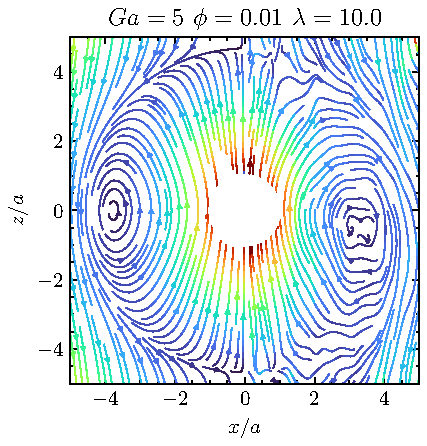
\includegraphics[width = 0.32\textwidth]{image/HOMOGENEOUS_final/Stream/Stream_PHI_1_Ga_5_l_10.pdf}
    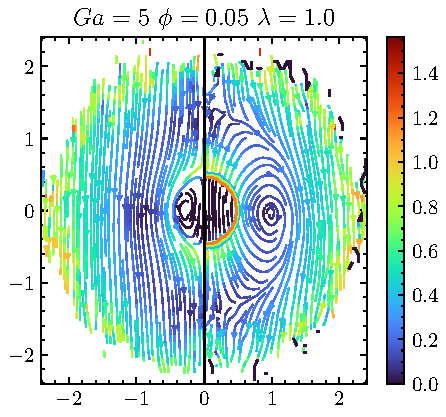
\includegraphics[width = 0.32\textwidth]{image/HOMOGENEOUS_final/Stream/Stream_PHI_5_Ga_5_l_10.pdf}
    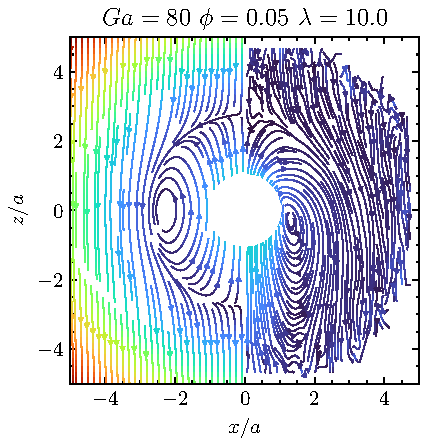
\includegraphics[width = 0.32\textwidth]{image/HOMOGENEOUS_final/Stream/Stream_PHI_5_Ga_80_l_10.pdf}
    \caption{Streamlines of the disturbance velocity field $\textbf{v}^\text{nst}$, in the cross-section given by the plane $(\textbf{e}_x,\textbf{e}_z)$, for two volume fractions $\phi = 0.01$ (left) and $\phi = 0.05$ (middle) at $\lambda = 10$ and $Ga = 5$.
    (right) plot of the inertial case $Ga = 80$. 
    On the left side of the panel ($x/a < 0$), we have re-plotted the theoretical solution provided by \ref{eq:v_nst_solution_adim}.   
    On the right side of the panel ($x/a > 0$), we have reconstructed the streamlines obtained with the DNS, using \ref{eq:vnst_DNS}. 
    The color map indicates the magnitude of the velocity, from black which corresponds to a velocity magnitude of 0, to the color at the interface of the droplet which corresponds to a magnitude of 1.}
    \label{fig:vnst_DNS}
\end{figure}
As seen on \ref{fig:vnst_DNS}:  %the common points that shear the velocity fields from the DNS to the theoretical prediction are the following: 
(1) both velocity fields exhibit approximately the same wake close to the interface of the droplet. 
That is the wake of an isolated rising vertical droplet. 
(2) For a distance large enough from the droplet center we see the downstream flow appears.
(3) The recirculation region, delimited by the null radial velocity (i.e. for the points $\textbf{r}$ following $\textbf{v}^\text{nst}\cdot \textbf{r} = 0$ with $|\textbf{r}|>a$), follows the same trends as the theoretical prediction, i.e. the radius is smaller for higher $\phi$. 
Additionally, the radii of the recirculation region have approximately the same size for both cases where $Ga = 5$. 

Regarding the differences, we can note that for the case $\phi = 0.01$, displayed on \ref{fig:vnst_DNS} (left) the wake of the particle is slightly asymmetric, while the theoretical solution is purely symmetric. 
The fore-aft symmetry of the wake of a particle as displayed in \ref{fig:vnst_vertical} is typically due to the absence of inertial effect. 
Thus, the non-fore-aft symmetry observed on the plot, \ref{fig:vnst_DNS} (left), is due to the non-negligible inertial effect present for this case. 
Indeed, as reported in \ref{tab:simulations_recall} the \textit{Reynolds} number for this case is $Re \approx 1$, implying that the inertial effects cannot be neglected. 
In opposition at $\phi = 0.05$, the numerical results exhibit a nearly fore-aft symmetric wake. 
This is consistent with the previous remark since for this case $Re < 1$. 

To extend our understanding we have also displayed on \ref{eq:vnst_DNS} (right) a high inertial case, with  $Ga = 80$. 
In this case, we see that the wake exhibits fore-aft asymmetry, which confirms that this trend comes with inertial effects. 
Additionally, we can note that the top boundary of the recirculation region is approximately at the same location as the theoretical prediction. 
However, the downstream boundary is different from the one predicted by the theoretical prediction, again that is because the fore-aft symmetry of the flow is broken.  
The symmetry of a distribution can be quantified by the ``skewness'' of the distribution. 
In the case of the continuous phase velocity distribution it is the triple velocity correlation $\avg{\chi_fk_f  \textbf{u}_f'}$ appearing in the pseudo turbulent energy equation \eqref{eq:dt_hybrid_k1}, that quantify the fore-aft symmetry.
As demonstrated, in Stokes regime $\avg{\chi_fk_f  \textbf{u}_f'} = 0$ due to the fore-after symmetry of the disturbance fields of spherical particles.  
Hence, the effect of inertia, which generates a fore-aft asymmetry in the particle's wake, will not necessarily impact the velocity variance but rather the skewness of the velocity distribution. 


To conclude, we can state that \ref{eq:v_nst_solution_adim} is well representative of the velocity field reconstructed with the DNS. 
Therefore, we can be confident regarding the accuracy of our \textit{Reynolds} stress closure at least for low \textit{Galileo} numbers. 




\subsection{Vertical velocity variance}

As discussed in the previous section, in the situation reproduced by the DNS, the velocity variance is given by \ref{eq:functional_form_avg} without the contribution of the buoyancy term (see \eqref{eq:cancelation1} and \ref{eq:cancelation2}). 
Additionally, for instance, we assert that the particle vertical velocity variance $\pavg{\textbf{u}_\alpha'\textbf{u}_\alpha'}_{zz}$ is negligible  at  $Ga =5$. 
In the next subsections, we show that this assumption is indeed confirmed by the DNS results. 
However, for the horizontal velocity variance, we will observe that it is not necessarily a valid assumption. 
Under these conditions, the vertical component of the velocity variance given by \ref{eq:functional_form_avg} is expressed as, 
\begin{equation}
    \frac{\avg{\chi_f \textbf{u}_f'\textbf{u}_f'}_{zz}}{\phi_f U^2}
    = \phi^{2/3} \left(
        \frac{2}{3}C_e^{(1)}+ C_e^{(2)}
    \right)
    = 
    \phi^{2/3}\Gamma\left(\frac{1}{3}\right) \frac{7}{60}\frac{(2+3\lambda)^2 }{(\lambda+1)^2}
    % \left(e^{-Re} - 1 \right)/2
    + \mathcal{O}(\phi), 
    % . 
    \label{eq:theoritical_simplified}
\end{equation}
where we recall that $\Gamma(1/3) \approx 2.67894$. 




\subsubsection{Comparison with the DNS}

In \ref{fig:uuyy} we compared the vertical velocity variance given by \ref{eq:theoritical_simplified} to the numerical results.
At low volume fraction and for all $\lambda$ very good agreements are obtained. 
Interestingly for all $\lambda$, \ref{eq:theoritical_simplified} seems to provide a good estimation for the Reynolds stress even at high volume fraction $\phi$, especially viscous droplets ($\lambda = 10$). 
Since no particle interaction terms of any kind are considered in the theory, this good agreement is likely coincidental.
\begin{figure}
    \centering
    % 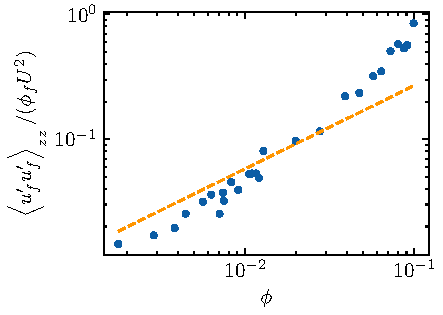
\includegraphics[height = 0.25\textwidth]{image/HOMOGENEOUS_final/CA/cartellier.pdf}
    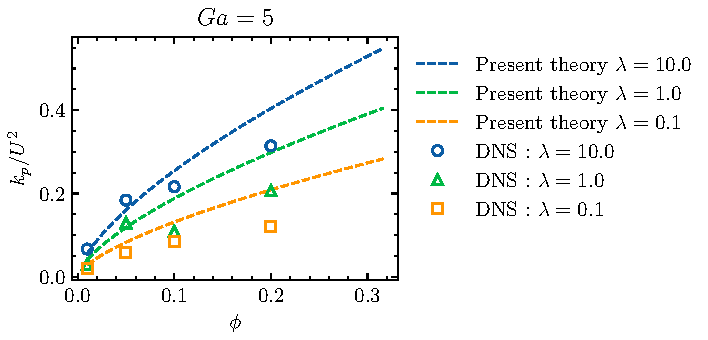
\includegraphics[height = 0.25\textwidth]{image/HOMOGENEOUS_final/CA/UUyy_Ga_5.pdf}
    \caption{Dimensionless value of the vertical velocity variance  in terms of the volume fraction $\phi$ for various $\lambda$ in the low inertial regime ($Ga = 5$). 
    % (left) Experimental  results  of \citet{cartellier2009induced} compared to \ref{eq:theoritical_simplified} with $\lambda = 0$ (dash dotted line) original scaling of \citet{cartellier2009induced}. 
    Comparison of the ``Present theory'' \eqref{eq:theoritical_simplified} against the velocity variance obtained with DNS results according to \eqref{eq:def_uuf_num}. 
    }
    \label{fig:uuyy}
\end{figure}
The red dashed line in \ref{fig:uuyy} (right) represents the potential flow solution of \citet{van1998pseudo} given by \ref{eq:van_wingarden_sol}. 
This model underpredicts the magnitude of the vertical pseudo-turbulence.
We deduce that the velocity variance produced by particles in Stokes flow is largely superior to in potential regime. 


\subsubsection{Comparison with the literature}

In \ref{fig:uuyy2}  we compare \ref{eq:theoritical_simplified} with $\lambda = 0$ to the  experimental measurements of \citet{cartellier2009induced}. 
We observe reasonable agreements from $\phi = 10^{-3}$ to moderate volume fraction ($\phi \approx 0.03$). 
In the low volume fraction regime \citet{cartellier2009induced} found that $\avg{\chi_f\textbf{u}_f'\textbf{u}_f'} / U^2 \sim \phi^{0.7 \pm 0.03}$,  while \ref{eq:theoritical_simplified} with $\lambda = 0$ predicts, $\avg{\chi_f\textbf{u}_f'\textbf{u}_f'} / U^2 \sim 1.25017 \cdot \phi^{2/3} $. 
Thus, our results overestimate \citet{cartellier2009induced} best fits by $25\%$. 
This can be explained by the non-negligible inertial effects present in \citet{cartellier2009induced} experiments, indeed they measured $Re \approx 10$ while our theory is valid in Stokes flow. 
\begin{figure}
    \centering
    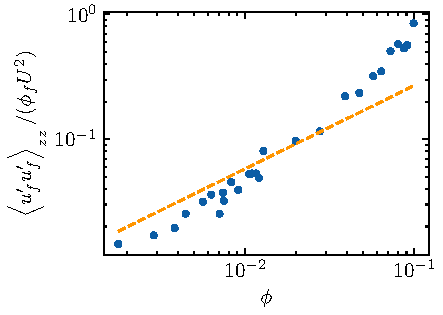
\includegraphics[height = 0.25\textwidth]{image/HOMOGENEOUS_final/CA/cartellier.pdf}
    \caption{Dimensionless value of the vertical velocity variance  in terms of the volume fraction $\phi$ for various $\lambda$ in the low inertial regime ($Ga = 5$). 
    (dots) Experimental  results  of \citet{cartellier2009induced}.
    (dashed line) Theoretical formula \ref{eq:theoritical_simplified} with $\lambda = 0$.
    (dash dotted line) \citet{cartellier2009induced}'s original scaling. 
    }
    \label{fig:uuyy2}
\end{figure}

It is reasonable to assume that the slight disparities observed between these results and the theory are due to the inertial effects or a non-negligible volume fraction effect. 
Thus, Considering the good agreements obtained with both, the numerical results and \citet{cartellier2009induced} experiments, we can state that \ref{eq:theoritical_simplified} is validated. 

\subsection{The Horizontal velocity variance}

Now that the vertical component of the velocity variance is validated, we turn our attention to the validation of the components in the normal direction to the gravity. 
Using the general formulation \ref{eq:functional_form_avg}, we write the horizontal component of the \textit{Reynolds} as, 
\begin{equation}
    \frac{\avg{\chi_f \textbf{u}_f'\textbf{u}_f'}_{xx}}{\phi_f U^2}
    = \phi^{2/3}\Gamma\left(\frac{1}{3}\right) \frac{1}{240}\frac{(2+3\lambda)^2 }{(\lambda+1)^2}
    + 
    C^{(1)}_e \left[
    \frac{\pavg{\textbf{u}_\alpha'\textbf{u}_\alpha'}_{xx}}{n_p U^2}
    - \frac{2k_p}{3U^2}  
    \right]
    + C^{(2)}_e
    \frac{2k_p}{U^2}  
    \label{eq:Horizontal_varience}
\end{equation}
Note how the first term on the right-hand side of \ref{eq:Horizontal_varience} is smaller than the one provided by \ref{eq:theoritical_simplified} ($1/240$ Vs. $7/60$). 
This means that the horizontal velocity variance produced by the mean vertical motion of the droplets is significantly lower than the vertical velocity variance. 
Additionally, in this formulation we have kept the terms related to the particle center of mass velocity variance. 


In \ref{fig:uuxx} (right) we display the numerical values of the horizontal velocity variance against the theoretical results provided by, \ref{eq:Horizontal_varience}. 
\begin{figure}
    \centering
    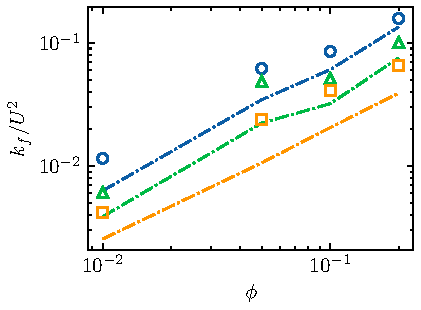
\includegraphics[height = 0.25\textwidth]{image/HOMOGENEOUS_final/CA/UUxx2_Ga_5.pdf}
    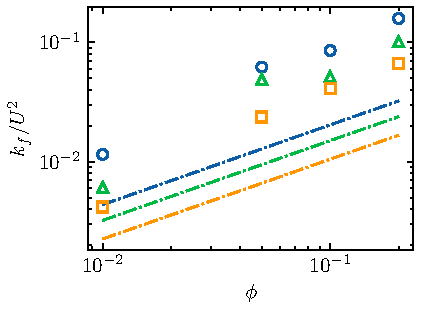
\includegraphics[height = 0.25\textwidth]{image/HOMOGENEOUS_final/CA/UUxx_Ga_5.pdf}
    \caption{Dimensionless value of the horizontal velocity varience  in terms of the volume fraction $\phi$ for various $\lambda$ in the low inertial regime ($Ga = 5$). 
    (left) Theoretical results \eqref{eq:Horizontal_varience} \underline{with} the particle velocity variance included
    (right) Theoretical results  \eqref{eq:Horizontal_varience} \underline{without} the particle velocity variance included. 
    }
    \label{fig:uuxx}
\end{figure}
It is seen that for all $\phi$ and $\lambda$ the theoretical predictions given by \ref{eq:Horizontal_varience}(right), when neglecting the particle phase velocity, i.e.  $k_p =0$ and $ \pavg{\textbf{u}_\alpha'\textbf{u}_\alpha'}_{xx} = 0 $, is underestimating the continuous phase velocity variance. 
Since the velocity variance produced by a Stokes disturbance field will be always larger (in dimensionless form) than the disturbance field given by an inertial particle, we must conclude that the lake of velocity variance predicted by the theory is due to the non-inclusion of the particle phase velocity variance. 
Indeed, according to \ref{fig:vnst_DNS} it seems that we can predict the effect of volume fraction on the averaged wake of the particle \eqref{eq:Horizontal_varience}.
Thus, the only reason why the fluid phase velocity variance is underestimated must be because of the absence of the particle phase velocity variance in this first approximation.  

On \ref{fig:uuxx} (left) we display the numerical values of the horizontal velocity variance against the theoretical results provided by, \ref{eq:Horizontal_varience}, including the values of $k_p$ and $\pavg{\textbf{u}_\alpha'\textbf{u}_\alpha'}_{xx}$ that is obtained with the DNS. 
The prediction in the dense regime ($\phi = 0.2$) seems greatly improved, while not many changes can be observed for the dilute regime. 
Indeed, in the dilute regime, we still obtain a significant error. 
At this stage it is hard to explain where does these differences come from however we can stipulate that the predicted magnitude of the velocity variance is greatly improved when including the particle phase center of mass variance. 

We can suppose that due to the relatively low magnitude of the horizontal velocity variance of the average wake of particles, the particle phase variance can no longer be neglected and must be accounted for. 
Thus, when developing an algebraic model for the \textit{Pseudo-turbulent} tensor, it is essential to consider the impact of the particle phase velocity variance, at least in the horizontal direction. 
Thus, a closure model for the particle phase velocity variance should be constructed first and incorporated into the \textit{Reynolds stress} model as outlined in \ref{eq:functional_form_avg} to remain consistent.

Nevertheless, in this chapter, we focus only on the modeling of the continuous phase velocity variance. 
We will model the particle phase velocity variance in the next chapter. 
Thus, in the subsequent sections, we make use of the particle center of mass velocity variance collected with the DNS to ensure a consistent modeling of the continuous phase \textit{Reynolds} stress.    


\subsection{Extension to higher inertial effects. }

In this subsection, we extend our model to higher \textit{Reynolds} numbers by making use of the DNS results. 
We assume the following properties to construct our semi-empirical model: 
(1) In the low inertial regime ($Re=0$) and low volume fraction ($\phi=0$) the \textit{Reynolds stress} must be given by  \ref{eq:functional_form_avg}. 
(2) The functional form given by \ref{eq:functional_form_avg} is preserved at finite $Re$ for the non-buoyancy terms. 
This means that the scalar $C_e^{(1)}$ and $C_e^{(2)}$ are the only degrees of freedom that we can use to include the finite inertial effects. 
(3) The semi-empirical expression  $C_e^{(1)}$ and $C_e^{(2)}$ should not take into account the effect of the particle phase velocity variance. 
Indeed, these are already taken into account through the terms $\pavg{\textbf{u}_\alpha'\textbf{u}_\alpha'}$ and $k_p$ in \ref{eq:functional_form_avg}. 
This means that we must perform a fit of $C_e^{(1)}$ and $C_e^{(2)}$ on the numerical data while including the particle velocity variance in \ref{eq:functional_form_avg}, that is directly obtained with the DNS.
In the subsequent chapter, we seek an analytical expression for $\pavg{\textbf{u}_\alpha'\textbf{u}_\alpha'}$ to close entirely \ref{eq:functional_form_avg} based on theoretical analysis.

In \ref{eq:functional_form_avg} the effects of inertia could be captured directly through the constant $A = Ga^2 /(12 Re)$. 
However, it has been found that this method yields no suitable results. 
This is because the formulation of $A$ is only valid in the Stokes flows. 
Indeed, \ref{eq:v_b_sol} is a singularity solution only valid in Stokes flows. 
Thus, we still consider that $C_k^{(2)}$ and $C_{ek}^{(2)}$ cancel-out according to \ref{eq:cancelation1} and \ref{eq:cancelation2} and play on the other parameters, i.e. $C_e^{(1)}$ and $C_e^{(2)}$,  to include inertial effects. 

In the following we first focus on the modeling of the trace of the \textit{Reynolds} stress, then once it is done we concentrate on the deviatoric part of this tensor. 

\subsubsection{The pseudo turbulent kinetic energy}

According to \ref{eq:functional_form_avg} the pseudo turbulent kinetic energy of the continuous phase can be written at $Re = 0$ and $\phi = 0$ by,
\begin{equation}
    k_f^{Re = 0}
    = 
    C_e^{(2)}  \left( U^2 + 2 k_p\right)  \frac{3}{2}
    % + \frac{3}{2} (C_k^{(2)} + C_{ek}^{(2)})
    \label{eq:TKE}
\end{equation}
We recall that in the stokes flow regime $C_k^{(2)}$ and $C_{ek}^{(2)}$ cancel-out. 
We propose the following semi-empirical formulation to express the fluid phase kinetic energy: 
\begin{equation}
    k_f
    = 
    k_f^{Re = 0}
    \cdot \frac{\left(e^{-Re} +1\right)}{2}.
    \label{eq:semi_empirical}
\end{equation}


In  \ref{fig:kf} we display the values of $k_f$ obtained with the DNS against the semi-empirical formula given by \ref{eq:semi_empirical} with (dot-dashed lines) and without (dashed lines) the particle phase velocity variance. 
We can observe that \ref{eq:semi_empirical} with the particle phase velocity variance included, fit reasonably all of our numerical results. 
We note that \ref{eq:semi_empirical} without $k_p$ (dashed lines) seem to underpredict the fluid phase velocity variance for $\phi = 0.2$. 
At lower volume fraction it is not clear whether it improves the predictions or not. 
Anyhow, for $\phi \le 0.1$ the particle phase velocity variance seems negligible compared to the averaged wake contribution. 

Consequently, this rather simple formula \eqref{eq:semi_empirical},  fits nicely all of our numerical results regardless of the viscosity ratio, \textit{Reynolds} numbers, and volume fraction.  
Thus, according to \ref{eq:semi_empirical}, it appears that the contribution of finite inertial effect leads to a reduction by a factor of 2 in the magnitude of the fluid phase kinetic energy when the \textit{Reynolds} number is large enough. 
Surprisingly, the dependence with $\phi$ and $\lambda$ do not seem to be affected by greater \textit{Reynolds} number, as witnessed by the absence of $\phi$ and $\lambda$ in \ref{eq:semi_empirical}. 
\begin{figure}
    \centering
    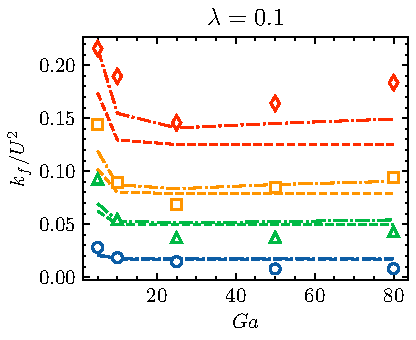
\includegraphics[height = 0.25\textwidth]{image/HOMOGENEOUS_final/CA/KF2_l_0.pdf}
    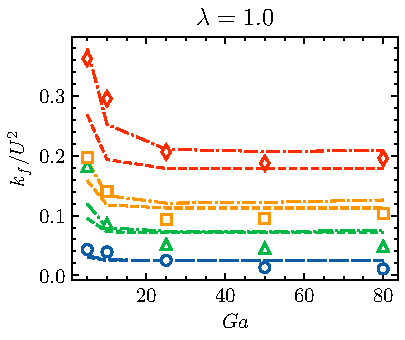
\includegraphics[height = 0.25\textwidth]{image/HOMOGENEOUS_final/CA/KF2_l_1.pdf}
    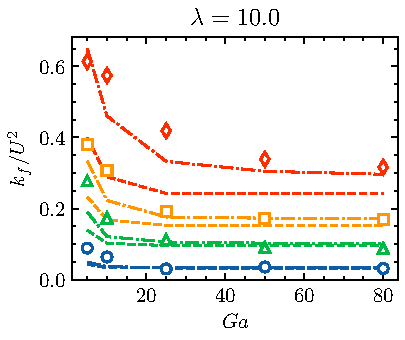
\includegraphics[height = 0.25\textwidth]{image/HOMOGENEOUS_final/CA/KF2_l_10.pdf}
    \caption{Dimensionless continuous phase pseudo turbulent energy, $k_f/U^2$ in terms of the \textit{Galileo} number.
    (left) $\lambda = 0.1$
    (middle) $\lambda = 1$
    (right) $\lambda = 10$
    (Symbols) DNS results computed according to \ref{eq:def_uuf_num}
    ($\pmb\bigcirc$) $\phi = 0.01$; ($\pmb\triangle$) $ \phi = 0.05$; ($\pmb\square$) $\phi = 0.1$ ($\pmb\lozenge$) $\phi = 0.2$.
    (dot-dashed lines) Semi-empirical formula \ref{eq:semi_empirical} \underline{including} the results of the DNS for the particle phase velocity fluctuations. 
    (dashed lines) Semi-empirical formula \ref{eq:semi_empirical} \underline{excluding} the particle phase velocity fluctuations. 
    }
    \label{fig:kf}
\end{figure}


\subsubsection{Deviatoric part of the Reynolds stress tensor}


From \ref{eq:functional_form_avg} we define the Deviatoric normalized part of the \textit{Reynolds Stress}, as, 
\begin{equation}
    \textbf{D} =
    \frac{3\avg{\chi_f\textbf{u}_f'\textbf{u}_f'}}{2 k_f} - 1
    = 
    b_f^{Re,\phi = 0} \left[
        \textbf{e}_p\textbf{e}_p
        + \frac{\pavg{\textbf{u}_\alpha'\textbf{u}_\alpha'}}{n_p U^2}
         - \frac{1}{3}(\textbf{e}_p\cdot \textbf{e}_p+2k_p/U^2)\bm\delta
    \right]
    \label{eq:D_def}
\end{equation}
Where the constant $b_f^{Re,\phi =0} = \frac{27}{10}$ in the Stokes and dilute regime \eqref{eq:constants}. 
To extend the domain of validity of \textbf{D} we must adjust the scalar $b_f^{Re,\phi = 0}$ to higher $Re$, and $\phi$.  


In \ref{fig:bf} we display the vertical (hollow symbols) and horizontal (filled symbols) components of $\textbf{D}$. 
It is shown that a good semi-empirical fit for $b_f$ is given by, 
\begin{equation}
    b_f = \frac{27}{10}  \text{exp}\left\{- 3\left(\phi^{5/6} + \frac{10^{-3}}{\lambda+1}Re\right)\right\}. 
    \label{eq:b_f}
\end{equation}
\begin{figure}
    \centering
    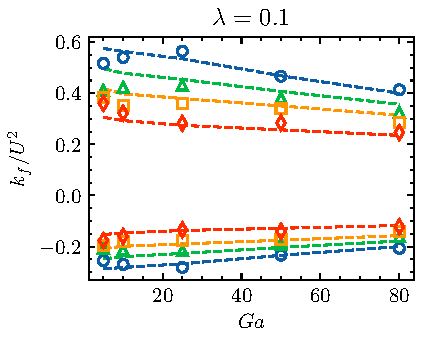
\includegraphics[height = 0.25\textwidth]{image/HOMOGENEOUS_final/CA/D2_l_0.pdf}
    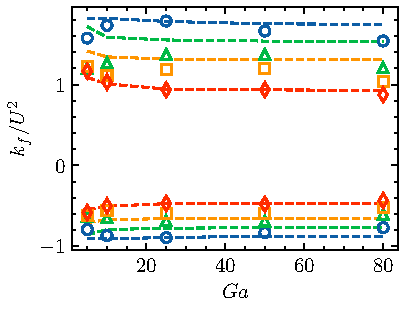
\includegraphics[height = 0.25\textwidth]{image/HOMOGENEOUS_final/CA/D2_l_1.pdf}
    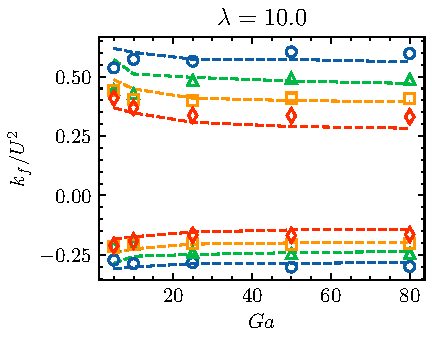
\includegraphics[height = 0.25\textwidth]{image/HOMOGENEOUS_final/CA/D2_l_10.pdf}
    \caption{Deviatoric part of the \textit{Reynolds stress} tensor, $\textbf{D}$, in terms of the \textit{Galileo} number for multiple viscosity ratios:
    (left) $\lambda = 0.1$,
    (middle) $\lambda = 1$,
    (right) $\lambda = 10$. 
    (Symbols) DNS results computed according to \ref{eq:def_uuf_num}, (hollow symbols) $\textbf{D}_{yy}$ and (filled symbols) $\textbf{D}_{xx}$. 
    (dot-dashed lines) Values of $\textbf{D}_{xx}$ given by \ref{eq:D_def} using \ref{eq:b_f}, including the particle phase velocity fluctuations obtained with the DNS. 
    (dashed lines) Values of $\textbf{D}_{yy}$ given by \ref{eq:D_def} using \ref{eq:b_f}
    ($\pmb\bigcirc$) $\phi = 0.01$; ($\pmb\triangle$) $ \phi = 0.05$; ($\pmb\square$) $\phi = 0.1$ ($\pmb\lozenge$) $\phi = 0.2$.
    }
    \label{fig:bf}
\end{figure}
We clearly observe that $b_f/b_f^{Re,\phi = 0}$ varies with $\phi$, $\lambda$ and the $Re$, while $k_f/k_f^{Re = 0}$ where just a function of $Re$. 
Specifically, for $\lambda = 10$ we observe that $b_f$ depends weakly on $Re$ or $Ga$, where it is a lot more dependent for bubbles. 

% This may be in contradiction with the results of \citet{mehrabadi2015pseudo} as his fitted constant $b_f$ is $Re$ dependent for solid sphere, i.e. $\lambda = \infty$. 
% Indeed, they $b_f$ reads in our notation as, 
% \begin{equation*}
%     \frac{0.523}{1+0.305 e^{-0.114}} \text{Exp}\left\{\frac{-3.511}{1+1.801 e^{-0.005Re(1-\phi)}}\right\}
% \end{equation*}
% This dispersencies in the results is still unclear to us.  


Although \ref{eq:b_f} and \ref{eq:semi_empirical} do not match exactly the numerical results, we prefer not to overfit our results and kept a rather simple fit for $b_f$ and $k_f$. 
In summary, with the constant $b_f$ and $k_f$ fitted on our numerical results we extended our \textit{Reynolds stress} model for higher $Re$, $\phi$, and $\lambda$. 
It must be remembered that since we studied only vertically rising buoyant bubbly flow we only extended the validity of this fit in this specific configuration. 



\subsection{Final validation}

We would like to end this section with a series of validations comparing our final model to the experimental and numerical results at finite \textit{Reynolds number}. 

On \ref{fig:trygvason} we first display the pseudoturbulence kinetic energy Vs. a series of numerical results from \citet{bunner2002dynamics,loisy2016direct,wang2021numerical} and experimental results of \citet{martinez2007measurement}.  
We can observe that the predicted magnitude of $k_f$ is in very good agreement with all these results. 
These studies concern either fixed arrays of particles or dilute suspensions of particles, in both cases the particle velocity variance is negligible, thus we consider that $k_p = 0$ in \ref{eq:semi_empirical}. 
We can observe that setting $\lambda \to\infty$ in \ref{eq:semi_empirical}, captures quantitatively the results of \citet{wang2021numerical} for solid particle fixed array. 
It also seems to correspond to the pseudo turbulence generated by the experimental results of \citet{martinez2007measurement} which considered rising bubbles in water. 
We assume that, because their bubbles are contaminated this can be considered as a no-slip boundary condition at the surface of the bubbles, which hence correspond to solid particles, i.e. $\lambda \to \infty$.  
\begin{figure}
    \centering
    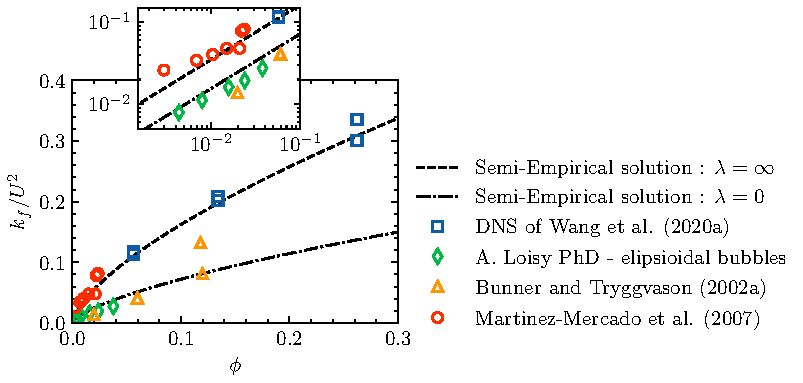
\includegraphics[height = 0.35\textwidth]{image/HOMOGENEOUS_final/CA/KFliterature.pdf}
    \caption{Dimensionless continuous phase pseudo turbulent energy, $k_f/U^2$ in terms of the \textit{Galileo} number.
    (Symbols) DNS and experimental results of: 
    ($\pmb\square$)  Particle-resolved Direct Numerical Simulations (PR-DNS)
    of fixed solid spherical particle assemblies at $20< Re < 100$  by \citet{wang2021numerical}; 
    ($\pmb\lozenge$) Direct numerical simulation (DNS) of rising deformable bubbles at $Re \approx 30$ \citep{loisy2016direct}
    ($\pmb\triangle$) DNS of rising spherical bubbles by \citet{bunner2002dynamics}. 
    ($\pmb\bigcirc$) Experiment of rising spherical bubbles in water by \citet{martinez2007measurement} at $Re \approx 30$. 
    (dot-dashed lines) Semi-empirical formula \ref{eq:semi_empirical} at $Re \approx 30$ with $\lambda = 0$. 
    (dashed lines)  Semi-empirical formula \ref{eq:semi_empirical} at $Re \approx 30$ with $\lambda = \infty$.
    }
    \label{fig:trygvason}
\end{figure}
In \ref{fig:trygvason} we also compared our analytical formula to the DNS results of \citet{bunner2002dynamics} and \citet{loisy2016direct} which considered rising bubbly flows. 
As can be seen from the (dashed lines) in \ref{fig:trygvason} our semi-empirical formula captures quantitatively their results. 

As the previous validation concerned the low but finite \textit{Reynolds number} regime, we now challenge ourselves and compare our semi-empirical formula \eqref{eq:semi_empirical} to DNS out of our range of \textit{Reynolds} numbers. 
In \citet{mehrabadi2015pseudo} they performed DNS of a fixed array of spherical solid spheres, from $Re_m = 1$ to $Re_m=300$ where $Re_m = (1- \phi) Re$ is the Reynolds number based on the mean slip velocity. 
\begin{figure}
    \centering
    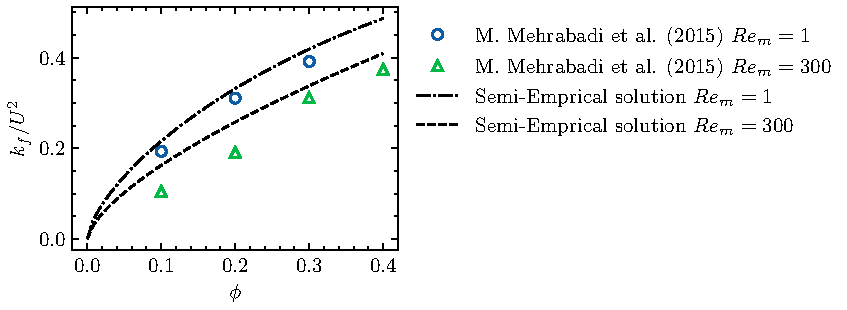
\includegraphics[height = 0.25\textwidth]{image/HOMOGENEOUS_final/CA/tenneti.pdf}
    \caption{Dimensionless continuous phase pseudo turbulent energy, $k_f/U^2$ in terms of the volume fraction $\phi$.
    (Symbols) 
    results of Particle-resolved Direct Numerical Simulations
    of fixed particle assemblies by \citet{mehrabadi2015pseudo}
    ($\pmb\bigcirc$) $Re_m = (1-\phi) \approx 1$; ($\pmb\triangle$) $Re_m \approx 300$;
    (dot-dashed lines) Semi-empirical formula \ref{eq:semi_empirical} at $Re_m = 1$
    (dashed lines) Semi-empirical formula \ref{eq:semi_empirical} at $Re_m = 300$
    }
    \label{fig:tennet}
\end{figure}
As shown in \ref{fig:tennet} (dot-dashed line), the results at low Reynolds number ($Re_m=1$) of \citet{mehrabadi2015pseudo}  correspond quantitatively to \eqref{eq:semi_empirical}. 
However, we can remark that at $Re_m = 300$, the relation $k_f \sim \phi^{2/3}$, seems not valid anymore, even at low $\phi$. 
This is evidenced by the empirical formula proposed by \citet{mehrabadi2015pseudo}, see Eq (7.1) of their paper. 
Nevertheless, it is remarkable that \ref{eq:semi_empirical} still provides a reasonable quantitative prediction, even at $Re_m = 300$. 


Finally, to validate the functional form of \ref{eq:functional_form_avg} regarding the inclusion of the particle phase velocity variance, we compare our results to the study of \citet{shajahan2023inertial}. 
They performed DNS of free arrays of solid particles under sedimentation.  
\begin{figure}
    \centering
    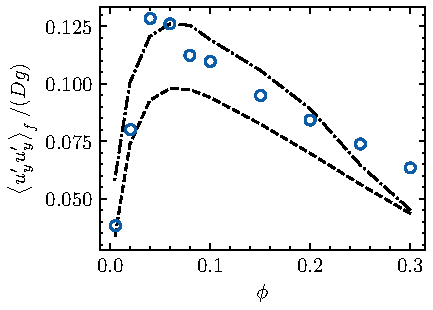
\includegraphics[height = 0.25\textwidth]{image/HOMOGENEOUS_final/CA/tariq.pdf}
    \caption{Dimensionless vertical velocity varience, in terms of the volume fraction $\phi$. 
    (Symbols) results of Particle-resolved Direct Numerical Simulations  of gravitational settling of monodisperse solid spheres by \citet{shajahan2023inertial} at $Ga = 144$. 
    (dot-dashed lines) Semi-empirical formula \underline{including} \citet{shajahan2023inertial}'s results for the particle phase velocity fluctuations. 
    (dashed lines) Semi-empirical formula \underline{excluding} the particle phase velocity fluctuations. 
    }
    \label{fig:tariq}
\end{figure}
We can observe on \ref{fig:tariq} (dashed lines) that the semi-emprical formula slightly underestimates the result when we neglect the particle phase velocity variance. 
When we include the contribution of the particle phase velocity variance (that we obtained in their study), we can note that the prediction improved a lot. 
We conclude that the general functional form of \ref{eq:functional_form_avg} seems to capture the dependence of the \textit{Reynolds} stress with the particle phase velocity variance. 

\section{What about the remaining terms and the C.L divergence paradox }

In \ref{chap:pseudoturbulence} we demonstrated that the Reynolds stress tensor could be expressed as,
\begin{equation}
    \avg{\chi_f \textbf{u}_f'\textbf{u}_f'}
    = 
    \phi_f
    \int_{\mathbb{R}^3}
    \textbf{v}_f^\text{nst}
    \textbf{v}_f^\text{nst}
    P_\text{nst}^f
    d\textbf{r}
    + 
    \phi_f
    \int_{\mathbb{R}^3}
    \textbf{v}_f^\text{nst}
    \textbf{v}_f^\text{nst}
    P_\text{nst}^f
    d\textbf{y}
    + 
    \int_{\mathbb{R}^3}
    \avg{
        \chi_f
        \textbf{u}_f''
        \textbf{u}_f''
        % \sum_i 
        % \delta(\textbf{x}+\textbf{y}-\textbf{x}_i)
        % \delta(\textbf{w}-\textbf{u}_i)
        % h_i
        \delta_\text{nst}
    }
    d\textbf{y}.
    \label{ap:eq:relation_ensemble_nst}
\end{equation}
For the sake of simplicity, in this appendix we consider that all droplets posses the same center of mass velocity $\textbf{u}_p$. 
Although the first term on the RHS can be computed at $\mathcal{O}(\phi)$ (see \ref{chap:pseudoturbulence}) no justifications have been provided to ensure that the second term could be neglected. 
In this appendix we demonstrate that, (1) the nearest particles' statistics formulation of the Reynolds stress \eqref{ap:eq:relation_ensemble_nst} leads to the same results as \citet{caflisch1985variance} if one consider the presence of the second term, and (2) that for periodic domain containing several droplets/particles, only the averaged wake of the nearest neighbor is predominant on the final result. 


\subsection{Zhang's idea}

\begin{equation}
    \avg{\textbf{u}'\textbf{u}'}
    =
    \int_{\mathbb{R}^3}\avg{\textbf{u}'\textbf{u}'\delta_{nst}} d\textbf{r}
\end{equation}
then derive directly an equation for $\textbf{u}'$ or $\textbf{u}_f'$. 

So i need $\textbf{u}^0\textbf{u}^0\delta_{nst}$ to which i subtract the equation for $\textbf{u} \textbf{u}$
that is to be computed with 
\begin{align}
    \label{eq:dt_rhou_k2}
    \pddt [\rho_k/2(u_k^0)^2]  
    + \div [\rho_k/2(u_k^0)^2\textbf{u}_k^0 - \textbf{u}_k^0 \cdot \bm{\sigma}_k^0]
    &=
    \rho_k\textbf{u}_k^0 \cdot \textbf{g}  
    -  \bm{\sigma}_k^0 : \grad \textbf{u}_k^0,
    \\
    \label{eq:dt_rhoe_k}
    \pddt (\rho_ke_k^0)  
    + \div (
        \rho_ke_k^0\textbf{u}_k^0
        + \textbf{q}_k^0
        )
    &= 
    \bm{\sigma}_k^0 : \grad \textbf{u}_k^0,
\end{align} 
\subsection{Contribution of the second-nearest droplet}

Using similar method to what is done for \ref{ap:eq:relation_ensemble_nst} we may demonstrate that,  
\begin{align*}
    \avg{\chi_f \textbf{u}_f'\textbf{u}_f'}[\textbf{x},t]
    &= 
    \int_{\mathbb{R}^3}
    \avg{\chi_f \textbf{u}_f'\textbf{u}_f' 
    \sum_i^N \delta(\textbf{x}_i - \textbf{x}- \textbf{r}_1)
    h_i
    }
    d\textbf{r}_1\\
    &= 
    \int_{\mathbb{R}^3}
    \int_{\mathbb{R}^3}
    \avg{\chi_f \textbf{u}_f'\textbf{u}_f' 
    \sum_i^N \delta(\textbf{x}_i - \textbf{x}- \textbf{r}_1)
    h_i
    \sum_{j\neq i}^N \delta(\textbf{x}_j - \textbf{x}- \textbf{r}_2)
    h_j
    }
    d\textbf{r}_2
    d\textbf{r}_1
\end{align*}
Doing so we arrive at the conslusion that, 
\begin{multline}
    \avg{\chi_f \textbf{u}_f'\textbf{u}_f'}
    = 
    \phi_f
    \int_{\mathbb{R}^3}
    \textbf{v}_f^\text{nst}
    \textbf{v}_f^\text{nst}
    P_\text{nst}^f
    d\textbf{r}_1
    + 
    \phi_f
    \int_{\mathbb{R}^6}
    \textbf{v}_f^\text{2-nst}
    \textbf{v}_f^\text{2-nst}
    P_\text{2-nst}^f
    d\textbf{r}_1
    d\textbf{r}_2 \\
    + 
    \int_{\mathbb{R}^6}
    \avg{
        \chi_f
        \textbf{u}_f'''
        \textbf{u}_f'''
        % \sum_i 
        % \delta(\textbf{x}+\textbf{y}-\textbf{x}_i)
        % \delta(\textbf{w}-\textbf{u}_i)
        % h_i
        \delta_\text{nst}
    }
    d\textbf{r}_1
    d\textbf{r}_2.
\end{multline}
where we have introduced the following notation, 
\begin{align}
    \phi_f
    &= 
    \avg{\chi_f}\\
    \phi_f P_\text{nst}^f 
    &= 
    \avg{\chi_f  
    \sum_i^N \delta(\textbf{x}_i - \textbf{x}- \textbf{r})
    h_i
    }\\
    \phi_f P_\text{nst}^f \textbf{u}_f^\text{nst}
    &= 
    \avg{\chi_f  
    \sum_i^N \delta(\textbf{x}_i - \textbf{x}- \textbf{r})
    h_i
    }\\
    \phi_f P_\text{2-nst}^f
    &= 
    \avg{\chi_f  
    \sum_i^N \delta(\textbf{x}_i - \textbf{x}- \textbf{r})
    h_i
    \sum_{j\neq i}^N \delta(\textbf{x}_j - \textbf{x}- \textbf{r})
    h_j
    }\\
    \phi_f P_\text{2-nst}^f \textbf{u}_f^\text{2-nst}
    &= 
    \avg{\chi_f \textbf{u}_f^0 
    \sum_i^N \delta(\textbf{x}_i - \textbf{x}- \textbf{r})
    h_i
    \sum_{j\neq i}^N \delta(\textbf{x}_j - \textbf{x}- \textbf{r})
    h_j
    }
\end{align}
where $P_\text{2-nst}^f[\textbf{r}_1, \textbf{r}_2|\textbf{x}]$ is the probability of finding the center of mass of the two nearest droplets to the point $\textbf{x}$ (being occupied by the continuous phase) at the location $\textbf{r}_1$ and $\textbf{r}_2$.  

Additionally, we introduce the disturbance velocity fields, 
\begin{align}
    \textbf{v}^\text{nst-f}_f[\textbf{r}_1,\textbf{x}] &= \textbf{u}^\text{nst-f}_f - \textbf{u}_f\\
    \textbf{v}^\text{2-nst-f}_f[\textbf{r}_1,\textbf{r}_2,\textbf{x}] &= \textbf{u}^\text{2-nst-f}_f - \textbf{u}_f^\text{nst-f}\\
    \textbf{v}'''_f &= \textbf{u}^0_f - \textbf{u}^\text{2-nst-f}_f
\end{align}
As discussed in the body of the text it is also useful to consider the bulk velocity evaluated at an arbitrary point \textbf{z}, knowing that the continuous phase is present at \textbf{x} and that the nearest neighbor to this point is present at $\textbf{r}_1$, and eventually that a second-nearest neighbor is present at $\textbf{r}_2$. 
Therefore, we introduce the fields, 
\begin{align}
    \textbf{v}^\text{nst-f}[\textbf{z}| \textbf{r}_1,\textbf{x}] &= \textbf{u}^\text{nst} - \textbf{u}\\
    \textbf{v}^\text{2-nst-f}[\textbf{z}| \textbf{r}_1,\textbf{r}_2,\textbf{x}] &= \textbf{u}^\text{2-nst} - \textbf{u}^\text{nst}\\
\end{align}
The alternative definitions of these fields are, 
\begin{align}
    P_\text{nst-f}^f \textbf{v}^\text{nst-f} &= \avg{ \textbf{u}^0 \left[\chi_f \sum_i^N \delta(\textbf{x}_i - \textbf{x}- \textbf{r})h_i - P_\text{nst}^f\right]}\\
    P_\text{2-nst-f}^f \textbf{v}^\text{2-nst-f} &= \avg{ \textbf{u}^0 \chi_f \sum_i^N \delta(\textbf{x}_i - \textbf{x}- \textbf{r})h_i \left[\sum_{j\neq i}^N \delta(\textbf{x}_j - \textbf{x}- \textbf{r}) h_j  - P_\text{2-nst}^\text{nst-f} \right] }
\end{align}
where $P_\text{2-nst}^\text{nst-f}$ is the probability of finding the second-nearest neighbor to \textbf{x} at $\textbf{r}_2$ knowing that the first nearest neighbor is already at $\textbf{r}_1$. 
For sake of brevity we introduce the notations, 
\begin{align}
    \delta_\text{nst-f}[\FF,t,\textbf{x},\textbf{r}_1] &\to \chi_f \sum_i^N \delta(\textbf{x}_i - \textbf{x}- \textbf{r})h_i \\
    \delta_\text{2-nst-f}[\FF,t,\textbf{x},\textbf{r}_1,\textbf{r}_2]  &\to  \chi_f \sum_i^N \delta(\textbf{x}_i - \textbf{x}- \textbf{r}_1)h_i \sum_{j\neq i}^N \delta(\textbf{x}_j - \textbf{x}- \textbf{r}_2) h_j  \\
    \delta_\text{nst-f}'[\FF,t,\textbf{x},\textbf{r}_1] &\to \chi_f \sum_i^N \delta(\textbf{x}_i - \textbf{x}- \textbf{r})h_i - P_\text{nst}^f\\
    \delta_\text{2-nst-f}'[\FF,t,\textbf{x},\textbf{r}_1,\textbf{r}_2]  &\to  \chi_f \sum_i^N \delta(\textbf{x}_i - \textbf{x}- \textbf{r}_1)h_i \left[\sum_{j\neq i}^N \delta(\textbf{x}_j - \textbf{x}- \textbf{r}_2) h_j  - P_\text{2-nst}^\text{nst-f} \right]
\end{align}
With this notation note that, 
\begin{align}
    \avg{\delta_\text{2-nst-f}'} &= 0\\
    P_\text{2-nst-f} \textbf{v}^\text{2-nst-f} &= \avg{\delta_\text{2-nst-f}' \textbf{u}^0}\\
    P_\text{2-nst-f} (\phi_f^\text{2-nst-f} -\phi_f^\text{nst-f}) &= \avg{\delta_\text{2-nst-f}' \chi_f}= - \avg{\delta_\text{2-nst-f}' \chi_d}= - P_\text{2-nst-f} (\phi_d^\text{2-nst-f} -\phi_d^\text{nst-f})
\end{align} 
The methodology to derive the mass and momentum equations governing $\textbf{v}^\text{nst}$ and $\textbf{v}^\text{2-nst}$ is then clear, we multiply the local single-fluid formulation of the momentum equation evaluated at a point \textbf{z} by $\delta_\text{2-nst-f}'$ or $\delta_\text{nst-f}'$, and ensemble average the resulting equations. 

In Stokes regime the single fluid formulation of the mass and momentum equations reads as, 
\begin{align}
    \div \textbf{u}^0 & =0 \\
    \div (\chi_f \bm\sigma_f^0 + \chi_d \bm\sigma_d^0 + \delta_\Gamma \bm\sigma_\Gamma^0)
    &=
    - (\chi_d \rho_d + \chi_f \rho_f) \textbf{g}
\end{align}
Averaging gives, 
\begin{align}
    \div \avg{\delta_\text{2-nst-f}' \textbf{u}^0} & =0 \\
    \div \avg{\delta_\text{2-nst-f}' (\chi_f \bm\sigma_f^0 + \chi_d \bm\sigma_d^0 + \delta_\Gamma \bm\sigma_\Gamma^0)}
    &=
    - \avg{\delta_\text{2-nst-f}'(\chi_d \rho_d + \chi_f \rho_f) \textbf{g}}
\end{align}

Then, noticing that, 
\begin{align*}
    \avg{\delta_\text{2-nst-f}' \chi_f \bm\sigma_f^0}
    =&
    -  P^f_\text{2-nst-f} \tau^\text{2-nst-f}_f \bm\delta
    + \mu_f P^f_\text{2-nst-f} \left[
        \grad \textbf{v}^\text{2-nst-f}
        + (\grad \textbf{v}^\text{2-nst-f})^\dagger
    \right]\\
    &- \avg{ \chi_d \delta_\text{2-nst-f}'\textbf{e}_d^0 } 
    % +  P^f_\text{2-nst-f} (\phi_d^\text{2-nst-f} p^\text{2-nst-f}_f - \phi_d^\text{nst-f} p^\text{nst-f})
    + \avg{\chi_d (p^\text{2-nst-f}_f \delta_\text{2-nst-f} - \delta_\text{nst-f}P_\text{2-nst}^\text{nst-f} p^\text{nst-f}_f )}\\
    \avg{\delta_\text{2-nst-f}'(\chi_d \rho_d + \chi_f \rho_f)}
    &=
    \avg{\delta_\text{2-nst-f}'\chi_d (\rho_d - \rho_f)}
\end{align*}
where $\tau^\text{2-nst}_f = p_f^\text{2-nst-f} - p_f^\text{nst-f}$ is the disturbance pressure field. 
For any tensor $\textbf{A}$ appearing under the divergence sign in the momentum equation we may write 
\begin{equation}
    \div\avg{\chi_d \textbf{A}}
    =
    \div\pOavg{\textbf{A}}
    -\frac{1}{2} \grad\grad : \pOavg{\textbf{Ar}+\textbf{rA}}
\end{equation}
Additionally, any integral of the stress, or moments of the stress may be written as, 
\begin{align*}
    \intO{
        \bm\sigma_d^0
    }
    + 
    \intS{
        \bm\sigma_\Gamma^0
    }
    &=
    \intS{\textbf{r}\bm\sigma_f^0 \cdot \textbf{n}}\\
    \intO{
        \textbf{r}\bm\sigma_d^0+ \textbf{r}\bm\sigma_d^0
    }
    + 
    \intS{
        \textbf{r}\bm\sigma_\Gamma^0+\textbf{r}\bm\sigma_\Gamma^0
    }
    &=
    \intS{\textbf{rr}\bm\sigma_f^0 \cdot \textbf{n}}
    + 
    \rho_d \intO{\textbf{rr}}
\end{align*}

Using this formulation for the stresses tensors and also for the pressure and internal shear tensor we arrive at the conclusion that, 
\begin{align}
    P_\text{2-nst-f}\div \textbf{u}^\text{2-nst-f} & =0 \\
    P_\text{2-nst-f}\div \bm\Sigma^\text{2-nst-f}
    &=
    P_\text{2-nst-f}\div \bm\sigma^\text{2-nst-f}_\text{eff}
    - \avg{\delta_\text{2-nst-f}'\delta_p  (\rho_d - \rho_f) \intO{}}
\end{align}
with the effective stress defined as, 
\begin{multline}
    \bm\sigma^\text{2-nst-f}_\text{eff}
    =
    - \avg{\delta_p \delta_\text{2-nst-f}'\intS{\textbf{r}\bm\sigma_f^0 \cdot \textbf{n}}}
    + \avg{\delta_p \delta_\text{2-nst-f}' \intO{\textbf{e}_d^0} }  \\
    -\bm\delta \avg{\delta_p \left(\intO{p^\text{2-nst-f}_f }\delta_\text{2-nst-f} - \delta_\text{nst-f}P_\text{2-nst}^\text{nst-f} \intO{p^\text{nst-f}_f} \right)}\\
    + \frac{1}{2}\div \left[
        \avg{\delta_p \delta_\text{2-nst-f}'\intS{\textbf{rr}\bm\sigma_f^0 \cdot \textbf{n}}}
        + \avg{\delta_p \delta_\text{2-nst-f}'\rho_f \intO{\textbf{rr}}}
    \right]\\
    + \frac{1}{2}\div \left[
        - \avg{\delta_p \delta_\text{2-nst-f}' \intO{\textbf{r}\textbf{e}_d^0+ \textbf{e}_d^0 \textbf{r}} }  \right. \\ \left. 
        - \avg{\delta_p \left(\intO{p^\text{2-nst-f}_f (\textbf{r}\bm\delta + \bm\delta \textbf{r})}\delta_\text{2-nst-f} - \delta_\text{nst-f}P_\text{2-nst}^\text{nst-f} \intO{p^\text{nst-f}_f (\textbf{r}\bm\delta + \bm\delta \textbf{r})} \right)}
    \right]
\end{multline}

\begin{align}
    P_\text{2-nst-f}[\textbf{r}_2,\textbf{r}_1,\textbf{x}]
    &= 
    P_\text{nst-f}[\textbf{r}_1,\textbf{x}]
    P_\text{2-nst-f}[\textbf{r}_2|\textbf{r}_1,\textbf{x}]
    = 
    \phi_f[\textbf{x}]
    P_\text{nst-f}[\textbf{r}_1|\textbf{x}]
    P_\text{2-nst-f}[\textbf{r}_2|\textbf{r}_1,\textbf{x}]\\
    P_\text{2--f}[\textbf{r}_2,\textbf{r}_1,\textbf{x}]
    &= 
    P_\text{1-f}[\textbf{r}_1,\textbf{x}]
    P_\text{2-f}[\textbf{r}_2|\textbf{r}_1,\textbf{x}]
    = 
    \phi_f[\textbf{x}]
    P_\text{1-f}[\textbf{r}_1|\textbf{x}]
    P_\text{2-f}[\textbf{r}_2|\textbf{r}_1,\textbf{x}]
\end{align}
Additionally, following \citet{zhang2021ensemble} we may now introduce, 
\begin{align}
    h_\text{1-nst}[\textbf{r}_1, \textbf{x}]
    =
    P_\text{nst-f}[\textbf{r}_1 , \textbf{x}] / P_\text{1-f}[\textbf{r}_1 ,\textbf{x}]
    = 
    P_\text{nst-f}[\textbf{r}_1 | \textbf{x}] /P_\text{1-f}[\textbf{r}_1 |\textbf{x}]
\end{align}
where $h_\text{2-nst}[\textbf{r}_1, \textbf{x}]$ is the probability of finding no particles center of mass in the spherical shell $a < |\textbf{z} - \textbf{x}| < |\textbf{r}_1 - \textbf{x}|$. 
Similarly
\begin{align}
    h_\text{2-nst}[\textbf{r}_2,\textbf{r}_1, \textbf{x}]
    =
    P_\text{2-nst-f}[\textbf{r}_2 ,\textbf{r}_1 , \textbf{x}] / P_\text{2-f}[\textbf{r}_2 ,\textbf{r}_1 ,\textbf{x}]
    =
    P_\text{2-nst-f}[\textbf{r}_2 |\textbf{r}_1 , \textbf{x}] 
    / 
    P_\text{2-f}[\textbf{r}_2 |\textbf{r}_1 ,\textbf{x}]
    h_\text{1-nst}
\end{align}
where $h_\text{2-nst}[\textbf{r}_2,\textbf{r}_1, \textbf{x}]$ is the probability that $\textbf{r}_1$ and $\textbf{r}_2$ are the nearest particles to \textbf{x}, knowing both particles are present and fluid at \textbf{x}. 
In other worlds it is the probability that no-other particles are present in the spherical shell $a < |\textbf{z} - \textbf{x}| < |\textbf{r}_1 - \textbf{x}|$ excluding the volume that the first particle occupy. 

Finally, 
\begin{equation}
    P_\text{2-nst-f}[\textbf{r}_2 ,\textbf{r}_1 , \textbf{x}] 
    =
    h_\text{2-nst}[\textbf{r}_2,\textbf{r}_1, \textbf{x}] 
    / h_\text{1-nst}[\textbf{r}_2,\textbf{r}_1 ]
    P_\text{2-f}[\textbf{r}_2 ,\textbf{r}_1 ,\textbf{x}]
\end{equation}
\paragraph*{Second option (may be better): }

\begin{equation}
    h_2[\textbf{r}_2,\textbf{r}_1,\textbf{x}]
    = 
    P_\text{2-nst-f}[\textbf{r}_2|\textbf{r}_1,\textbf{x}]
    / 
    P_\text{2-f}[\textbf{r}_2|\textbf{r}_1,\textbf{x}]
\end{equation}
So that $h_2$ is the probability of finding no particle for the points \textbf{z} in the region $|\textbf{r}_1- \textbf{x}|<|\textbf{z}- \textbf{x}|<|\textbf{r}_2- \textbf{x}|$, making the particle 2 the second closested. 



\paragraph*{Summary}

\begin{equation}
    P_\text{2-nst-f}
    = 
    \phi_f 
    P_\text{nst-f}
    P_\text{2-nst-f}
    = 
    \phi_f 
    h_1 P_\text{1-f}
    h_2 P_\text{2-f}
\end{equation}
In the dilute regime where there is no overlap it is easy to compute all of these terms. 


To compute the probability $h_1$ it is easy. 
It is one minus th proba of finding a particle in the volume $V$. 
In that case the volume is, 
\begin{equation}
    V = \frac{4}{3}\pi (r_1^3 - a^3)
\end{equation}
then we introduce the infinitesimal volume $dv = V / N$. The probability of finding a part in sucha small volume is $n_p v$ and thus, 
\begin{equation}
    h_1 
    = \lim_{N\to\infty}
    (1-n_p \frac{V}{N})^N 
    = e^{-n_p V}
\end{equation}

\begin{tikzpicture}

    % Define points
    \coordinate (X) at (0,0); % Center X
    \coordinate (r1) at (3,0); % Point r1
    \coordinate (r2) at (2.6,3); % Point r2 (farther than r1)

    % Dashed circles centered at X
    \draw[dashed] (X) circle (1); % Dashed circle from X to r1
    \draw[dashed] (X) circle (3); % Dashed circle from X to r1
    \draw[dashed] (X) circle (4); % Dashed circle from X to r2
    \draw[dashed] (r1) circle (2); % Dashed circle from X to r2

    % Solid circle centered at r1 with radius 2a
    \draw[thick] (r1) circle (2);

    % Shaded region between r1 and r2, excluding the solid circle
    \begin{scope}
        \clip (r1) circle (2);
        % \fill (X) circle (6);
    \end{scope}

    % Draw labels
    \fill (X) circle (2pt) node[left] {\Large $\textbf{x}$};
    \fill (r1) circle (2pt) node[below] {\Large $\textbf{r}_1$};
    \fill (r2) circle (2pt) node[below] {\Large $\textbf{r}_2$};

\end{tikzpicture}

The same reasoning can be made for $h_2$ except that the volume in question is, 
\begin{equation}
    V = \{
        |\textbf{r}_1 - \textbf{x}| < |\textbf{z} - \textbf{x}| < |\textbf{r}_2 - \textbf{x}|
        \setminus
        |\textbf{z} - \textbf{r}_1| < 2a
    \}
\end{equation}
For consistness we intriducde 
\begin{equation}
    V = \{
        r_1 < |\textbf{z} - \textbf{x}| < r_2
        \setminus
        |\textbf{z} - \textbf{r}_1| < 2a
    \}
\end{equation}
We must find the volume of the spherical caps. 
The volume of the spherical shell excluding the sphere at $\textbf{r}_1$ can be computed as, 
\begin{equation}
    V 
    = 
    \int_0^{2\pi}
    \int_{r_1}^{r_2}
    \int_{\theta_{min}(r)}^{\pi}
    r^2
    \sin\theta
    d\theta 
    dr
    d\varphi
\end{equation}
where we have choosen a local coordinate system centered at $\textbf{x}$ in the direction of $\textbf{r}_1$. 
In this situation the eq of the surface of the sphere at $\textbf{r}_1$ might be written, 
\begin{align}
    x^2
    + y^2
    + (z-r_1)^2
    &= (2a)^2\\
    r^2 \sin^2\theta_{min}
    + (r \cos\theta_{min} -r_1)^2
    &= (2a)^2\\
    - r^2 
    + 2 \cos\theta_{min} r r_1 
    - r_1^2
    &= - (2a)^2\\
    + 2 \cos\theta_{min} r r_1 
    &= 
    r^2 
    + 
    (r_1+2a)(r_1-2a)
\end{align}
Thus, 
\begin{equation}
    \theta_{min}
    = \left\{
    \begin{tabular}{ll}
        $\arccos\{
        \frac{
            r^2 
            + r_1^2
             - (2a)^2
        }{2 r r_1}\}
        $&$
        \forall r < (r_1+2a)$\\
        $ 
        0
        $&$
        \forall r > (r_1+2a)$
    \end{tabular}
    \right.
\end{equation}


So for points $r_2 <r_1 +2a$ the integration goes like, 
\begin{align}
    V 
    &= 
    \int_0^{2\pi}
    d\varphi
    % \left[
    \int_{r_1}^{r_2}
    \int_{\theta_{min}(r)}^{\pi}
    % +
    %     \int_{r_1+2a}^{r_2}
    %     \int_{0}^{\pi}
    % \right]
    r^2
    \sin\theta
    d\theta 
    dr\\
    &= 
    \pi /r_1
    \int_{r_1}^{r_2} 
    [2r^2r_1 +  
        r^3 
        + r(r_1^2
        - (2a)^2)
    ]
    dr\\
    &= 
    \pi /r_1
    [2r^3/3r_1 
        +  r^4/4
        + r^2/2 (r_1^2 - (2a)^2)
    ]_{r_1}^{r_2} \\
    &= 
    \pi /r_1
    [\frac{2r_1}{3}(r_2^3-r_1^3) 
    + \frac{1}{4} (r_2^4-r_1^4)
        + \frac{1}{2}(r_2^2 - r_1^2) (r_1^2 - (2a)^2)]\\
    & = \frac{4\pi}{3}
    \frac{ 
     8 r_{1} \left(r_{2}^{3} - r_{1}^{3}\right) 
    + 3 (r_{2}^{4} - r_{1}^{4})
    + 6  \left(r_{1}^{2} - (2 a)^{2} \right) \left(r_{2}^{2} - r_{1}^{2}\right)}{16 r_{1}}
\end{align}

For points $r_2 > r_1 +2a$ we have, 
\begin{align}
    V &= 
    \pi /r_1
    [\frac{2r_1}{3}((r_1 + 2a)^3-r_1^3) 
    + \frac{1}{4} ((r_1 + 2a)^4-r_1^4)
        + \frac{1}{2}((r_1 + 2a)^2 - r_1^2) (r_1^2 - (2a)^2)]
    \\
    &+\frac{4\pi}{3}(r_2^3 - (r_1+(2a)^3))\\
    &
    =
    \frac{4\pi}{3}\left[
        -\frac{3a^4}{r_1}
        - 4 a^3 
        + r_2^3
        -r_1^3
    \right]
\end{align}

Assuming $r_1/a \to r_1$ and $r_2/a \to r_2$ we have, 
\begin{align}
    V 
    &= 
    \frac{4\pi a^3}{3}
    \frac{ 
     8 r_{1} \left(r_{2}^{3} - r_{1}^{3}\right) 
    + 3 (r_{2}^{4} - r_{1}^{4})
    + 6  \left(r_{1}^{2} - 4 \right) \left(r_{2}^{2} - r_{1}^{2}\right)}{16 r_{1}}
    \\
    V 
    &= 
    \frac{4\pi a^3}{3}\left[
        -\frac{3}{r_1}
        - 4 
        + r_2^3
        -r_1^3
    \right]
\end{align}



We conclude that, 
\begin{align}
    h_1 &= \exp\left\{-\phi (r_1^3 - 1)\right\}& \forall r_1 > a\\
    h_2 &= \exp\left\{-\phi 
        \frac{ 
        8 r_{1} \left(r_{2}^{3} - r_{1}^{3}\right) 
       + 3 (r_{2}^{4} - r_{1}^{4})
       + 6  \left(r_{1}^{2} - 4 \right) \left(r_{2}^{2} - r_{1}^{2}\right)}{16 r_{1}}
    \right\} &\forall  r_2 < r_1 + 2\\ 
    h_2 &= \exp\left\{-\phi 
    \left[
        -\frac{3}{r_1}
        - 4 
        + r_2^3
        -r_1^3
    \right]
    \right\} &\forall  r_2 > r_1 + 2 
\end{align}

\paragraph*{Results : }
For the $r_2 < r_1 + 2$ we have, 
\begin{equation}
    P_{2-nst}^f[\textbf{r}_2 | \textbf{r}_1,\textbf{x}]
    = 
    n_p[\textbf{r}_2]
    \exp\left\{-\phi 
        \frac{ 
        8 r_{1} \left(r_{2}^{3} - r_{1}^{3}\right) 
       + 3 (r_{2}^{4} - r_{1}^{4})
       + 6  \left(r_{1}^{2} - 4 \right) \left(r_{2}^{2} - r_{1}^{2}\right)}{16 r_{1}}
    \right\} 
\end{equation}
and for $r_2 > r_1 + 2$
\begin{equation}
    P_{2-nst}^f[\textbf{r}_2 | \textbf{r}_1,\textbf{x}]
    = 
    n_p[\textbf{r}_2]
    \exp\left\{-\phi 
    \left[
        -\frac{3}{r_1}
        - 4 
        + r_2^3
        -r_1^3
    \right]
    \right\} 
\end{equation}
and for both cases $P_{2-nst}^f = 0 $ for $r_2 < r_1$ and $|\textbf{r}_2-\textbf{r}_1|<2a$. 
Note that we should have 
\begin{equation}
    \int_{
        r_1 < r_2
        \setminus
        |\textbf{r}_2 - \textbf{r}_1| < 2a
    }
    P_{2-nst}^f[\textbf{r}_2 | \textbf{r}_1,\textbf{x}]
    d\textbf{r}_2 
    = 1 
\end{equation}


\paragraph*{Check : }

\begin{equation}
    \int_{
        \mathcal{D}_1 + \mathcal{D}_2
    }
    P_{2-nst}^f
    d\textbf{r}_2 
    = 
    \int_{
        \mathcal{D}_1 
    }
    P_{2-nst}^f
    d\textbf{r}_2 
    + 
    \int_{
        \mathcal{D}_2
    }
    P_{2-nst}^f
    d\textbf{r}_2 
\end{equation}

The first integral, 
\begin{multline}
    \int_{
        \mathcal{D}_1 
    }
    P_{2-nst}^f
    d\textbf{r}_2 
    \\=
    \frac{3 \phi}{4\pi}
    \int_0^{2\pi}
    \int_{r_1}^{r_1+2}
    \int_{\theta_{min}}^{\pi}
    \exp\left\{-\phi 
    \frac{ 
    8 r_{1} \left(r_{2}^{3} - r_{1}^{3}\right) 
   + 3 (r_{2}^{4} - r_{1}^{4})
   + 6  \left(r_{1}^{2} - 4 \right) \left(r_{2}^{2} - r_{1}^{2}\right)}{16 r_{1}}
    \right\} 
    r_2^2
    \sin\theta
    d\theta
    d\varphi
    dr_2
    \\=
    \frac{3 \phi}{4\pi}
    \int_0^{2\pi}
    \int_{r_1}^{r_1+2}
    \exp\left\{-\phi 
    \frac{ 
    8 r_{1} \left(r_{2}^{3} - r_{1}^{3}\right) 
   + 3 (r_{2}^{4} - r_{1}^{4})
   + 6  \left(r_{1}^{2} - 4 \right) \left(r_{2}^{2} - r_{1}^{2}\right)}{16 r_{1}}
    \right\} 
    r_2^2
    [-\cos\theta]_{\theta_{min}}^{\pi}
    d\varphi
    dr_2
    \\=
    \frac{3 \phi}{4\pi}
    2\pi
    \int_{r_1}^{r_1+2}
    r_2^2
    [1
    + \frac{
        r_2^2 
        + r_1^2
         - 4
    }{2 r_2 r_1}]
    \exp\left\{-\phi 
    \frac{ 
    8 r_{1} \left(r_{2}^{3} - r_{1}^{3}\right) 
   + 3 (r_{2}^{4} - r_{1}^{4})
   + 6  \left(r_{1}^{2} - 4 \right) \left(r_{2}^{2} - r_{1}^{2}\right)}{16 r_{1}}
    \right\} 
    dr_2
    \\=
    \frac{3 \phi}{4\pi}
    \frac{\pi}{r_1}
    \int_{r_1}^{r_1+2}
    [2r_2^2r_1
    + 
        r_2^3
        + r_2 (r_1^2
         - 4)]
    \exp\left\{-\phi 
    \frac{ 
    8 r_{1} \left(r_{2}^{3} - r_{1}^{3}\right) 
   + 3 (r_{2}^{4} - r_{1}^{4})
   + 6  \left(r_{1}^{2} - 4 \right) \left(r_{2}^{2} - r_{1}^{2}\right)}{16 r_{1}}
    \right\} 
    dr_2
    \\
    =
    1 
    - 
    \exp\left\{
        -\phi (6r_1^2 + 12 r_1 + 4 - \frac{3}{r_1})
        \right\}
\end{multline}

The second integral, 
\begin{multline}
    \int_{
        \mathcal{D}_2 
    }
    P_{2-nst}^f
    d\textbf{r}_2 
    =
    \frac{3 \phi}{4\pi}
    \int_0^{2\pi}
    \int_{r_1+2}^\infty
    \int_{0}^{\pi}
    \exp\left\{-\phi 
    \left[
        -\frac{3}{r_1}
        - 4 
        + r_2^3
        -r_1^3
    \right]
    \right\} 
    r_2^2
    \sin\theta
    d\theta
    d\varphi
    dr_2 \\
    =
    3 \phi
    \int_{r_1+2}^{\infty}
    \exp\left\{-\phi 
    \left[
        -\frac{3}{r_1}
        - 4 
        + r_2^3
        -r_1^3
    \right]
    \right\} 
    r_2^2
    dr_2 \\
    = \exp\left\{
        - \phi [
            6 r_1 
            + 12 r_1
            + 4
            - \frac{3}{r_1}
        ]
    \right\}
\end{multline}

We obtain indeed, 

\begin{equation}
    \int_{
        \mathcal{D}_1 + \mathcal{D}_2
    }
    P_{2-nst}^f
    d\textbf{r}_2 
    = 
    1
\end{equation}


\subsubsection{Evaluation of the effect of a second nearest part on the RS}

In the first place let us introduce the relation, 
\begin{align*}
    \avg{\chi_f \textbf{u}_f'\textbf{u}_f'}[\textbf{x},t]
    &= 
    \int_{\mathbb{R}^3}
    \avg{\chi_f \textbf{u}_f'\textbf{u}_f' 
    \sum_i^N \delta(\textbf{x}_i - \textbf{x}- \textbf{r}_1)
    h_i
    }
    d\textbf{r}_1\\
    &= 
    \int_{\mathbb{R}^3}
    \textbf{v}_f^\text{nst}
    \textbf{v}_f^\text{nst}
    P_f^\text{nst}
    d\textbf{r}_1
    + 
    \int_{\mathbb{R}^3}
    \avg{\chi_f \textbf{u}_f''\textbf{u}_f'' 
    \sum_i^N \delta(\textbf{x}_i - \textbf{x}- \textbf{r}_1)
    h_i
    }
    d\textbf{r}_1
    % \int_{\mathbb{R}^3}
    % \int_{\mathbb{R}^3}
    % \avg{\chi_f \textbf{u}_f'\textbf{u}_f' 
    % \sum_i^N \delta(\textbf{x}_i - \textbf{x}- \textbf{r})
    % h_i
    % \sum_{j\neq i}^N \delta(\textbf{x}_j - \textbf{x}- \textbf{r}_2)
    % h_j
    % }
    % d\textbf{r}_2
    % d\textbf{r}_1
\end{align*}
where $\textbf{u}_f'' = \textbf{u}_f^0 - \textbf{u}_f^\text{nst}$. 

Then, notice that the second term can be further expressed as, 
\begin{align}
    \avg{\chi_f \textbf{u}_f''\textbf{u}_f'' 
    \sum_i^N \delta(\textbf{x}_i - \textbf{x}- \textbf{r}_1)
    h_i
    }
    = 
    \int 
    \avg{\chi_f \textbf{u}_f''\textbf{u}_f'' 
    \sum_i^N \delta(\textbf{x}_i - \textbf{x}- \textbf{r}_1)h_i
    \sum_{j\neq i }^N \delta(\textbf{x}_j - \textbf{x}- \textbf{r}_2)h_j
    }
    d\textbf{r}_2\\
    =
    \int 
    \textbf{v}_f^\text{2-nst}
    \textbf{v}_f^\text{2-nst}
    P_\text{2-nst-f}
    d\textbf{r}_2
    + 
    \int 
    \avg{\chi_f \textbf{u}_f'''\textbf{u}_f''' 
    \sum_i^N \delta(\textbf{x}_i - \textbf{x}- \textbf{r}_1)h_i
    \sum_{j\neq i }^N \delta(\textbf{x}_j - \textbf{x}- \textbf{r}_2)h_j
    }
    d\textbf{r}_2
\end{align}
Where, $\textbf{u}_f''' = \textbf{u}_f^0 - \textbf{u}_f^\text{2-nst}$ and, 
\begin{equation}
    \textbf{v}_f^\text{2-nst}[\textbf{r}_2,\textbf{r}_1,\textbf{x}]
    = 
    \textbf{u}_f^\text{2-nst}[\textbf{r}_2,\textbf{r}_1,\textbf{x}]
    - \textbf{u}_f^\text{nst}[\textbf{r}_1,\textbf{x}]
\end{equation}
which might be obtained as, 
\begin{equation}
    \textbf{v}_f^\text{2-nst} P_\text{f-nst-2}
    = 
    (
    \textbf{u}_f^\text{2-nst}
    - \textbf{u}_f^\text{nst}
    )P_\text{f-nst-2}
    = 
    \avg{
        \chi_f \textbf{u}_f^0 \delta_\text{nst}
        (
            \delta_{nst-2}
            - P_\text{nst-2}^\text{f-nst}
        )
    }
\end{equation}
Anyhow the int can be expressed as, 

\begin{multline}
    \int 
    \textbf{v}_f^\text{2-nst}
    \textbf{v}_f^\text{2-nst}
    P_\text{2-nst-f}
    d\textbf{r}_2
    = 
    P_\text{nst-f}
    \int 
    \textbf{v}_f^\text{2-nst}
    \textbf{v}_f^\text{2-nst}
    P_2^\text{nst-f}
    d\textbf{r}_2\\
    = 
    P_\text{nst-f}
    \int 
    \mathcal{O}(\bm\delta/r_2^2)
    P_2^\text{nst-f}
    d\textbf{r}_2
\end{multline}
since $\textbf{v}_f^\text{2-nst}$ does not contains the mean effect of the particle in $r_1$ it is a most $\mathcal{O}(1/r_2)$.

Thus, the final contribution of this term is, 
\begin{multline}
    \int      P_\text{nst-f}
    \int 
    \mathcal{O}(1/r_2^2)
    P_2^\text{nst-f}
    d\textbf{r}_2
    d\textbf{r}_1
\end{multline}
We recall that, 
\begin{equation}
    P_\text{nst-f}
    = \frac{4\phi}{3\pi}
    \exp{[-\phi (r_1^3 - 1)]}
\end{equation}
Such that, 
\begin{multline}
    \int     \frac{4\phi}{3\pi}
    \exp{[-\phi (r_1^3 - 1)]}
    \int 
    \mathcal{O}(1/r_2^2)
    P_2^\text{nst-f}
    d\textbf{r}_2
    d\textbf{r}_1
\end{multline}

This integral can be computed into the two respective region of integration, yielding, 

The first integral, 
\begin{multline}
    \int_{
        \mathcal{D}_1 
    }
    \frac{1}{r_2^2}P_{2-nst}^f
    d\textbf{r}_2 
    =\\
    \frac{3 \phi}{4\pi}
    \frac{\pi}{r_1}
    \int_{r_1}^{r_1+2}
    [2r_1
    + 
        r_2
        +     
        \frac{1}{r_2}
        (r_1^2 - 4)]
    \exp\left\{-\phi 
    \frac{ 
    8 r_{1} \left(r_{2}^{3} - r_{1}^{3}\right) 
   + 3 (r_{2}^{4} - r_{1}^{4})
   + 6  \left(r_{1}^{2} - 4 \right) \left(r_{2}^{2} - r_{1}^{2}\right)}{16 r_{1}}
    \right\} 
    dr_2\\
\end{multline}

The second integral, 
\begin{multline}
    \int_{
        \mathcal{D}_2 
    }
    \frac{1}{r_2^2}P_{2-nst}^f
    d\textbf{r}_2 
    =
    3 \phi
    \int_{r_1+2}^{\infty}
    \exp\left\{-\phi 
    \left[
        -\frac{3}{r_1}
        - 4 
        + r_2^3
        -r_1^3
    \right]
    \right\} 
    dr_2 
\end{multline}



\subsection*{$N^{th}$ nearest neighbor}

\begin{equation}
    \avg{
        \chi_f \textbf{u}_f' \textbf{u}_f'
    }
    =
    \int d \textbf{r}^N \avg{
        \chi_f \textbf{u}_f' \textbf{u}_f'
        \prod_{k=0}^{N-1} \sum_{i_k \neq i_{k-1},i_{k-2},\ldots, i_0}^{N-k}
        \delta(\textbf{x}_{i_k} - \textbf{x} - \textbf{r}_k)
        h_{i_k}
    }
\end{equation}
The conditional field, 
\begin{equation}
    \textbf{u}^{N-nst} P_{N-nst}
    = 
    \sum_i^N (1+\grad^2) \mathcal{G}(\textbf{r}_i)+\ldots
\end{equation}



\subsection*{conditional eq for the two-nearest neighbor equaiton}


For consistness we note, 
\begin{align}
    \chi_f[\textbf{x}] \sum_i \delta(\textbf{x}_i-\textbf{x}-\textbf{r}_1)h_i
    &\to 
    \delta_\text{f-nst}[\textbf{x},\textbf{r}_1]\\
    \chi_f[\textbf{x}] 
    \sum_i \delta(\textbf{x}_i-\textbf{x}-\textbf{r}_1)h_i
    \sum_{j\neq i} \delta(\textbf{x}_i-\textbf{x}-\textbf{r}_2)h_j
    &\to 
    \delta_\text{f-2-nst}[\textbf{x},\textbf{r}_1,\textbf{r}_2]\\
\end{align}
We need an equaiton for the velocity field, 
\begin{equation}
    \textbf{v}_f^\text{2-nst}P_\text{f-2-nst}
    =
    \avg{
        \textbf{u}_f^0 
        (\delta_\text{2-nst-f} - \delta_\text{nst-f} P^\text{nst-f}_\text{2-nst})
    }
\end{equation}
At the points $\textbf{x}$ note that $\textbf{v}_f^\text{2-nst} = \textbf{v}^\text{2-nst}$ with,
\begin{equation}
    (\textbf{v}^\text{2-nst}P_\text{f-2-nst})[\textbf{z},\textbf{x},\textbf{r}_1,\textbf{r}_2]
    =
    \avg{
        \avg{
            \textbf{u}^0[\textbf{z}]
            (\delta_\text{2-nst-f} - \delta_\text{nst-f} P^\text{nst-f}_\text{2-nst})
        }
    }
\end{equation}

In order to be even more concise we note,
\begin{equation}
    \delta_\text{2-nst-f} - \delta_\text{nst-f} P^\text{nst-f}_\text{2-nst}
    \to 
    \Pi_\text{2-nst-f}^\text{nst-f}
\end{equation}


The local scale equaitons, 
\begin{align}
    \div \textbf{u}^0  &= 0 \\
    \rho_f \pddt \textbf{u}^0
    + \rho_f \div \textbf{u}^0\textbf{u}^0
    &= 
    \div \bm\sigma^* 
    + \rho_f \textbf{g}
    + \kappa \delta_\Gamma(\bm\sigma_f^0 \cdot \textbf{n})
\end{align}
with 
\begin{align}
    \bm\sigma^0 
    &= \chi_f \bm\sigma_f^0
    + \chi_f \bm\sigma_d^0/\zeta
    + \delta_\Gamma \bm\sigma_\Gamma^0/\zeta\\
    \zeta
    &= \rho_d / \rho_f\\
    \kappa
    &= (1-\zeta)/\zeta\\
\end{align}

Multiplying the right-hand side (Stokes eq) by  $\Pi_\text{2-nst-f}^\text{nst-f}$ and averaging yields, 
\begin{align}
    \div (P_\text{2-nst-f} \textbf{v}^\text{2-nst-f}) &= 0 \\
    \div \bm\sigma_\text{2-nst-f}^\text{eff}
    &= 
    - \kappa  \avg{\Pi_\text{2-nst-f}^\text{nst-f} \delta_\Gamma(\bm\sigma_f^0 \cdot \textbf{n})}
\end{align}
with, 
\begin{align}
    \bm\sigma_\text{2-nst-f}^\text{eff}
    &= 
    \avg{\Pi (\chi_f \bm\sigma_f^0
    + \chi_f \bm\sigma_d^0/\zeta
    + \delta_\Gamma \bm\sigma_\Gamma^0/\zeta
    )}\\
    &= 
    - P_\text{2-nst-f} \tau_f^\text{2-nst-f} \bm\delta
    +\mu_f P_\text{2-nst-f} (
        \grad \textbf{v}^\text{2-nst-f}
        + ^\dagger\grad \textbf{v}^\text{2-nst-f}
    )\\
    &+ P_\text{2-nst-f} (\phi_d^{nst} p_f^\text{2-nst-f} -\phi_d^{nst} p_f^\text{nst-f})
    + \avg{\Pi(+ \chi_f (\bm\sigma_d^0/\zeta - 2\mu_f \textbf{e}_d^0)
    + \delta_\Gamma \bm\sigma_\Gamma^0/\zeta)}
\end{align}
where $\tau$ is the disturbance pressure field $\tau^\text{2-nst-f}_f = p^\text{2-nst-f}_f - \tau^\text{nst-f}_f$.
Expanding the drag force term etc and keeping only the homogeneous terms yields,
\begin{align}
    \bm\sigma_\text{2-nst-f}^\text{eff}
    &= 
    \avg{\Pi (\chi_f \bm\sigma_f^0
    + \chi_f \bm\sigma_d^0/\zeta
    + \delta_\Gamma \bm\sigma_\Gamma^0/\zeta
    )}\\
    &= 
    - P_\text{2-nst-f} \tau_f^\text{2-nst-f} \bm\delta
    +\mu_f P_\text{2-nst-f} (
        \grad \textbf{v}^\text{2-nst-f}
        + ^\dagger\grad \textbf{v}^\text{2-nst-f}
    )\\
    &
    % + P_\text{2-nst-f} (\phi_d^{nst} p_f^\text{2-nst-f} -\phi_d^{nst} p_f^\text{nst-f})
    + \pavg{\Pi \intS[i]{\textbf{r}\bm\sigma_f^0\cdot \textbf{n} -2\mu_f \textbf{e}_d^0}}\\
    &-\frac{1}{2}\div  \left[
        \pavg{\Pi \intS[i]{\textbf{rr}\bm\sigma_f'\cdot \textbf{n} -2\mu_f (\textbf{r}\textbf{e}_d^0+\textbf{e}_d^0 \textbf{r})}}
        + \pavg{\Pi} \textbf{V} \rho_f \textbf{g}
    \right]
\end{align}
Indeed, in stokes flow regime we have, 
\begin{multline}
    \intO{ \textbf{r}(\bm{\sigma}^0_d)_{ik}+r_{k}(\bm{\sigma}^0_d)_{ji}}
    +\intS{ \textbf{r}(\bm{\sigma}^0_I)_{ik}+r_{k}(\bm{\sigma}_\Gamma^0)_{ji}}
    = 
    \intS{  \textbf{rr} (\bm{\sigma}_f^0\cdot\textbf{n}_d)_i }
    + \intO{ \textbf{rr}  \rho_d \textbf{g} } 
    \label{eq:dt_P2_alpha_bis}
\end{multline}



Accoring to the relation, 
\begin{equation}
    (\delta_\Gamma \ldots)[\textbf{z}]
    =
    \sum_k \delta(\textbf{x}_k - \textbf{z}) \intS{\ldots}
    - \div \sum_k \delta(\textbf{x}_k - \textbf{z}) \intS{\textbf{r}\ldots}
    % +\frac{1}{2} \grad\grad : \sum_i \delta(\textbf{x}_i - \textbf{z}) \intS{\textbf{rr}\ldots}
\end{equation}
Additionally, the product, 
\begin{align}
    \Pi_\text{2-nst-f}^\text{nst-f}
    \sum_i \delta(\textbf{x}_i - \textbf{z}) 
    &= 
    \chi_f[\textbf{x}] 
    \sum_i \delta(\textbf{x}_i-\textbf{x}-\textbf{r}_1)h_i
    \sum_{j\neq i} \delta(\textbf{x}_i-\textbf{x}-\textbf{r}_2)h_j
    \sum_k \delta(\textbf{x}_k - \textbf{z}) \\
    &- 
    P^\text{nst-f}_\text{2-nst}\chi_f[\textbf{x}] 
    \sum_i \delta(\textbf{x}_i-\textbf{x}-\textbf{r}_1)h_i
    % \sum_{j\neq i} \delta(\textbf{x}_i-\textbf{x}-\textbf{r}_2)h_j
    \sum_k \delta(\textbf{x}_k - \textbf{z}) \\
    &= 
    \chi_f[\textbf{x}] 
    \sum_i \delta(\textbf{x}_i-\textbf{x}-\textbf{r}_1)h_i
    \sum_{j\neq i} \delta(\textbf{x}_i-\textbf{x}-\textbf{r}_2)h_j
    [ \delta(\textbf{x}_j - \textbf{z}) +  \delta(\textbf{x}_i - \textbf{z})  + \sum_{k\neq i,j} \delta(\textbf{x}_k - \textbf{z}) ]\\
    &- P^\text{nst-f}_\text{2-nst}\chi_f
    \sum_i \delta(\textbf{x}_i-\textbf{x}-\textbf{r}_1)h_i
    [\delta(\textbf{x}_i - \textbf{z})  + \sum_{k\neq i} \delta(\textbf{x}_k - \textbf{z}) ]\\
\end{align}
Under the avg operator it is clear that, 
\begin{multline}
    \avg{(\ldots)\Pi_\text{2-nst-f}^\text{nst-f} \sum_i \delta(\textbf{x}_i - \textbf{z}) }
    =
    \delta(\textbf{r}_1 - \textbf{z}) \avg{(\ldots)\Pi_\text{2-nst-f}^\text{nst-f} }
    % -\delta(\textbf{r}_1 - \textbf{z}) P^\text{nst-f}_\text{2-nst} \avg{(\ldots)\delta_\text{2-nst-f}}\\
    +\delta(\textbf{r}_2 - \textbf{z}) \avg{(\ldots)\delta_\text{2-nst-f}}\\
    + \avg{(\ldots)\delta_\text{2-nst-f} \sum_{k\neq i,j} \delta(\textbf{x}_k - \textbf{z}) }
    - P^\text{nst-f}_\text{2-nst} \avg{(\ldots) \delta_\text{nst-f} \sum_{k\neq i} \delta(\textbf{x}_k - \textbf{z}) }\\
\end{multline}

In Stokes regime we may write, 
\begin{equation*}
    \intS[i] {\bm\sigma_f^0 \cdot \textbf{n}} =
    \rho_d \textbf{g} v
\end{equation*}
where $v=v_i$ for mono-disperse suspenison. 
Thus we obtain, 
\begin{multline}
    \avg{\Pi_\text{2-nst-f}^\text{nst-f} \sum_i \delta(\textbf{x}_i - \textbf{z}) \intS[i] {\bm\sigma_f^0 \cdot \textbf{n}}}
    =
    % \delta(\textbf{r}_1 - \textbf{z}) \avg{\rho_d \textbf{g} v \Pi_\text{2-nst-f}^\text{nst-f} }
    % -\delta(\textbf{r}_1 - \textbf{z}) P^\text{nst-f}_\text{2-nst} \avg{(\ldots)\delta_\text{2-nst-f}}\\
    + \rho_d \textbf{g} v \delta(\textbf{r}_2 - \textbf{z}) P_\text{2-nst-f}\\
    + \rho_d \textbf{g} v \avg{\delta_\text{2-nst-f} \sum_{k\neq i,j} \delta(\textbf{x}_k - \textbf{z}) 
    -  P^\text{nst-f}_\text{2-nst} \delta_\text{nst-f} \sum_{k\neq i} \delta(\textbf{x}_k - \textbf{z}) }\\
    =
    % \delta(\textbf{r}_1 - \textbf{z}) \avg{\rho_d \textbf{g} v \Pi_\text{2-nst-f}^\text{nst-f} }
    % -\delta(\textbf{r}_1 - \textbf{z}) P^\text{nst-f}_\text{2-nst} \avg{(\ldots)\delta_\text{2-nst-f}}\\
    + P_\text{2-nst-f} \rho_d \textbf{g} v \delta(\textbf{r}_2 - \textbf{z}) 
    - P_\text{2-nst-f} \rho_d \textbf{g} v n_p \int_{r_1<|\textbf{z}' - \textbf{x}| <r_2} \delta(\textbf{z}'-\textbf{z})d\textbf{z}\\
\end{multline}

\begin{multline}
    \avg{\textbf{V}\rho_f \textbf{g}\Pi_\text{2-nst-f}^\text{nst-f} \sum_i \delta(\textbf{x}_i - \textbf{z}) }
    =
    % \delta(\textbf{r}_1 - \textbf{z}) \avg{\textbf{V}\rho_f \textbf{g}\Pi_\text{2-nst-f}^\text{nst-f} }
    % -\delta(\textbf{r}_1 - \textbf{z}) P^\text{nst-f}_\text{2-nst} \avg{\textbf{V}\rho_f \textbf{g}\delta_\text{2-nst-f}}\\
    +\textbf{V}\rho_f \textbf{g}\delta(\textbf{r}_2 - \textbf{z}) \avg{\delta_\text{2-nst-f}}\\
    +\textbf{V}\rho_f \textbf{g} \avg{\delta_\text{2-nst-f} \sum_{k\neq i,j} \delta(\textbf{x}_k - \textbf{z}) }
    -\textbf{V}\rho_f \textbf{g} P^\text{nst-f}_\text{2-nst} \avg{ \delta_\text{nst-f} \sum_{k\neq i} \delta(\textbf{x}_k - \textbf{z}) }\\
    =
    + P_\text{2-nst-f} \bm\delta V \rho_f \textbf{g}\delta(\textbf{r}_2 - \textbf{z}) 
    - P_\text{2-nst-f} \bm\delta V \rho_f \textbf{g} n_p \int_{r_1<|\textbf{z}' - \textbf{x}| <r_2} \delta(\textbf{z}'-\textbf{z})d\textbf{z}
\end{multline}


Let call $S$ the stress on the particle $i$ then,
\begin{multline}
    \avg{\textbf{S}_k\Pi_\text{2-nst-f}^\text{nst-f} \sum_k \delta(\textbf{x}_k - \textbf{z}) }
    =
    \delta(\textbf{r}_1 - \textbf{z}) \avg{\Pi_\text{2-nst-f}^\text{nst-f}  \textbf{S}_i}
    % -\delta(\textbf{r}_1 - \textbf{z}) P^\text{nst-f}_\text{2-nst} \avg{\textbf{S}_k\delta_\text{2-nst-f}}\\
    +\delta(\textbf{r}_2 - \textbf{z}) \avg{\delta_\text{2-nst-f} \textbf{S}_j}\\
    + \avg{\delta_\text{2-nst-f} \sum_{k\neq i,j} \delta(\textbf{x}_k - \textbf{z}) \textbf{S}_k }
    - P^\text{nst-f}_\text{2-nst} \avg{\delta_\text{nst-f} \sum_{k\neq i} \delta(\textbf{x}_k - \textbf{z}) \textbf{S}_k }\\
    = 
    \delta(\textbf{r}_1 - \textbf{z}) (\textbf{S}_{1}^\text{2-nst-f} - \textbf{S}_{1}^\text{nst-f}) P_\text{2-nst-f}
    + \delta(\textbf{r}_2 - \textbf{z}) \textbf{S}_2^\text{2-nst-f} P_\text{2-nst-f}\\
    + P_\text{2-nst-f} n_p \int_{r_2 < |\textbf{z}' - \textbf{z}|}\textbf{S}[\textbf{z}'|\textbf{r}_1,\textbf{r}_2,\textbf{x}]\delta(\textbf{z}'-\textbf{z})d\textbf{z}
    - P_\text{2-nst-f} n_p \int_{r_1 < |\textbf{z}' - \textbf{z}|}\textbf{S}[\textbf{z}'|\textbf{r}_1,\textbf{x}] \delta(\textbf{z}'-\textbf{z}) d\textbf{z}
\end{multline}
if one assume that $\textbf{S}[\textbf{z}'|\textbf{r}_1,\textbf{r}_2,\textbf{x}] = \textbf{S}[\textbf{z}'|\textbf{r}_1,\textbf{x}]$ in the region $r_2 > |\textbf{z}-\textbf{x}|$ posses the same formula then 
\begin{multline}
    \avg{\textbf{S}_k\Pi_\text{2-nst-f}^\text{nst-f} \sum_k \delta(\textbf{x}_k - \textbf{z}) }
    =
    \delta(\textbf{r}_1 - \textbf{z}) (\textbf{S}_{1}^\text{2-nst-f} - \textbf{S}_{1}^\text{nst-f}) P_\text{2-nst-f}
    + \delta(\textbf{r}_2 - \textbf{z}) \textbf{S}_2^\text{2-nst-f} P_\text{2-nst-f}\\
    % + P_\text{2-nst-f} n_p \int_{r_2 < |\textbf{z}' - \textbf{z}|}\textbf{S}[\textbf{z}'|\textbf{r}_1,\textbf{r}_2,\textbf{x}]\delta(\textbf{z}'-\textbf{z})d\textbf{z}
    % - P_\text{2-nst-f} n_p \int_{r_2 < |\textbf{z}' - \textbf{z}|}\textbf{S}[\textbf{z}'|\textbf{r}_1,\textbf{x}] \delta(\textbf{z}'-\textbf{z}) d\textbf{z}
    - P_\text{2-nst-f} n_p \int_{r_1 < |\textbf{z}' - \textbf{z}|<r_2}\textbf{S}[\textbf{z}'|\textbf{r}_1,\textbf{x}] \delta(\textbf{z}'-\textbf{z}) d\textbf{z}
\end{multline}
Note that the terms with $\delta(\textbf{r}_{1,2} - \textbf{z})$ in factor arent funciton of $\textbf{z}$ them selfs thus the final eq might be written, (when $P_\text{2-nst-f}\neq =0$)
\begin{align}
     \div \textbf{v}^\text{2-nst-f} &= 0 \\
    - \grad\tau_f^\text{2-nst-f} 
    +\mu_f \grad^2\textbf{v}^\text{2-nst-f}
    = 
    &- (\rho_f - \rho_d) \textbf{g} v \delta(\textbf{r}_2 - \textbf{z}) \\
    &+ (\rho_f - \rho_d) \textbf{g} v n_p \int_{r_1<|\textbf{z}' - \textbf{x}| <r_2} \delta(\textbf{z}'-\textbf{z})d\textbf{z} \\
    &-  (\textbf{S}_{1}^\text{2-nst-f} - \textbf{S}_{1}^\text{nst-f})  \cdot \grad \delta(\textbf{r}_1 - \textbf{z}) \\
    &-  \textbf{S}_2^\text{2-nst-f}  \cdot \grad \delta(\textbf{r}_2 - \textbf{z}) \\
    &+  n_p \int_{r_1 < |\textbf{z}' - \textbf{z}|<r_2}\textbf{S}[\textbf{z}'|\textbf{r}_1,\textbf{x}] \cdot \grad\delta(\textbf{z}'-\textbf{z}) d\textbf{z}\\
    &+ \frac{1}{2} V \rho_f \textbf{g}\grad^2\delta(\textbf{r}_2 - \textbf{z}) \\
    &- \frac{1}{2} V \rho_f \textbf{g} n_p \int_{r_1<|\textbf{z}' - \textbf{x}| <r_2} \grad^2\delta(\textbf{z}'-\textbf{z})d\textbf{z} \\
\end{align}


\subsection{Recursive demonstration with simplified PDF}
Let us consider the pdf, 
\begin{equation}
    P_n [\textbf{r}_n \ldots \textbf{r}_1|\textbf{x}]
    = 
    \frac{3\phi}{4\pi} e^{-\phi (r_n^3 -  1)}
\end{equation}
Equally we may use the notation , 
\begin{equation}
    P_n [\textbf{r}_n | \textbf{r}_{n-1} \ldots, \textbf{r}_1, \textbf{x}]
    = 
    \frac{3\phi}{4\pi} e^{-\phi (r_n^3 -  (r_{n-1}))}
\end{equation}

Using the decomposition etc we obtain 
\begin{align}
    \avg{\chi_f \textbf{u}_f'\textbf{u}_f'}/ \phi_f
    &=
    \int_{0}^{\infty}
    \left\{
        \textbf{u}^1
        \textbf{u}^1
        P_1 
        +
        \int_{r_1}^{\infty}
        \left[
        \textbf{u}^2
        \textbf{u}^2
        P_2 
        + \ldots
        \textbf{u}^{n-1}
        \textbf{u}^{n-1}
        P_{n-1}
        + 
        \int_{r_{n-1}}^{\infty}
        \textbf{u}^n
        \textbf{u}^n
        P_n
        \ldots
        d\textbf{r}_n 
        \right]
        d\textbf{r}_2
    \right\}
    d\textbf{r}_1 \\
    &=
    \sum_{i=1}^N 
    \prod_{k=1}^i \left(
        P_{k_{k-1}}
        \int_{r_{k-1}}^{\infty}
        d\textbf{r}_k 
    \right)
    \textbf{u}^i
    \textbf{u}^i
\end{align}


Assuming $u^i$ is the stokslet of the part in $i^{th}$ wehavegot, 
\begin{equation}
    (\textbf{u}^i )^2
     = 1/r_i^2
\end{equation}
\begin{align}
    \avg{\chi_f \textbf{u}_f'\cdot \textbf{u}_f'}/ \phi_f
    &=
    \sum_{i=1}^N 
    \prod_{k=1}^{i+1} \left(
        4\pi r_k^2
        \int_{r_{k-1}}^{\infty}
        d\textbf{r}_k 
    \right)
    \frac{1}{r_{i+1}^2}
    e^{-\phi(r_{i+1}^3- 1)}\\
    &=
    \sum_{i=1}^N 
    \prod_{k=1}^{i+1} \left(
        4\pi r_k^2
        \int_{r_{k-1}}^{\infty}
        d\textbf{r}_k 
    \right)
    \frac{1}{r_{i+1}^2}
    e^{-\phi(r_{i+1}^3- 1)}\\
\end{align}


\subsection{Finite sized domain. }


\begin{figure}[h!]
    \centering
    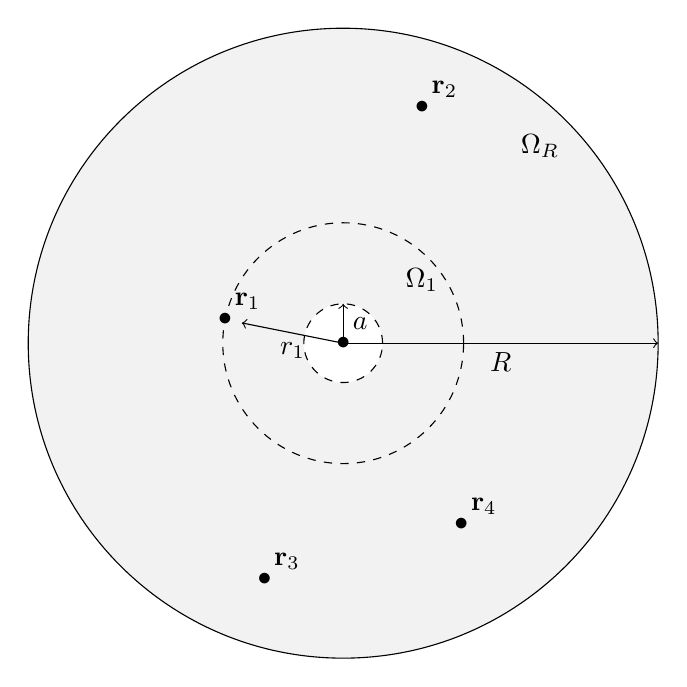
\begin{tikzpicture}
        \draw[fill=gray!10] (0,0) circle (4);
        \draw[dashed,fill=white] (0,0) circle (0.5);
        \draw[->](0,0)--(4,0)node[midway,below]{$R$};
        \draw[->](0,0)--(0,0.5)node[midway,right]{$a$};
        \node (O) at (0,0){$\bullet$}; 
        \node (r1) at (-1.5,0.3){$\bullet$}; 
        \node (r2) at (1,3){$\bullet$}; 
        \node (r3) at (-1,-3){$\bullet$}; 
        \node (r4) at (1.5,-2.3){$\bullet$}; 
        \draw (r1) node [above right] {$\textbf{r}_1$};
        \draw (r2) node [above right] {$\textbf{r}_2$};
        \draw (r3) node [above right] {$\textbf{r}_3$};
        \draw (r4) node [above right] {$\textbf{r}_4$};
        \draw[->] (0,0) -- (r1) node [midway, below] {$r_1$};
        \node  at (2.5,2.5){$\Omega_R$}; 
        \draw[dashed] (0,0) circle (1.529);
        \node  at (1,0.8){$\Omega_1$}; 
    \end{tikzpicture}
\end{figure}
We assume that, 
\begin{itemize}
    \item The number of droplets /particles in the domain is constant and is noted $N$. 
    Droplets might rise and go out the domain however we assume that the same number go inside at the same time as the domain is supposed either physical or periodic, or large enough. 
    \item The size of the domain $\Omega_R$ is $4/3 \pi R^3$
    \item All the length can be made dimensionless with the radius of a droplet noted $a$.
\end{itemize}


\subsubsection{Decomposition of the 2points nearest particle statistics probability}

We search to compute the probability distrbution $P_\text{2-nst-f}[\textbf{r}_1,\textbf{r}_2,\textbf{x}]$ defined as, 
\begin{align}
    \phi_f
    &= 
    \avg{\chi_f}\\
    \phi_f P^f_1
    &= 
    \avg{\chi_f \sum_{i=1}^{N}\delta(\textbf{x}_i - \textbf{x} - \textbf{r})}\\
    \phi_f P_\text{nst}^f =
    \phi_f P_1^f h_\text{nst}^\text{1-f}
    &= 
    \avg{\chi_f  
    \sum_i^N \delta(\textbf{x}_i - \textbf{x}- \textbf{r})
    h_i
    }\\
    \phi_f P_\text{2-nst}^f
    &= 
    \avg{\chi_f  
    \sum_i^N \delta(\textbf{x}_i - \textbf{x}- \textbf{r})
    h_i
    \sum_{j\neq i}^N \delta(\textbf{x}_j - \textbf{x}- \textbf{r})
    h_j
    }
\end{align}

This distribution can be decomposed as, 
\begin{equation}
    P_\text{nst-f-2}
    =
    \phi_f
    P_\text{nst}^f
    P_\text{2-nst}^\text{nst-f}
\end{equation}
Each of these distributions can then be decomposed as, 
\begin{align}
    P_\text{nst}^f
    &=
    P_\text{1}^f
    h^\text{1-f}_\text{nst}\\
    P_\text{2-nst}^\text{nst-f}
    &=
    P_\text{2}^\text{nst-f}
    h^\text{2-f}_\text{nst}
\end{align}
where, 
\begin{itemize}
    \item $P_\text{1}^f$ is the probability of finding a particle at $\textbf{r}_1$ knowing the continuous phase is at $\textbf{x}$
    \item $h^\text{1-f}_\text{nst}$ is the probability that the particle at $\textbf{r}_1$ is the nearest one to the point \textbf{x} knowing that there is indeed a particle at $\textbf{r}_1$ and the fluid at \textbf{x}. 
    \item $P_\text{2}^\text{nst-f}$ is the probability of finding a particle at $\textbf{r}_2$ knowing the continuous phase is at $\textbf{x}$ and the nearest particle to \textbf{x} is at $\textbf{r}_1$. 
    \item $h^\text{2-f}_\text{nst}$ is the probability that the particle at $\textbf{r}_2$ is the second-nearest one to the point \textbf{x} knowing that there is indeed a particle at $\textbf{r}_1$ and the fluid at \textbf{x}. 
\end{itemize}

\subsubsection{Unconditional number density}
The probability of finding a particle center of mass in a small element $d\textbf{x}$ around a point \textbf{x} is, 
\begin{equation}
    n_p(\textbf{x}+ \textbf{r})
    = \avg{\sum_{i=1}^N \delta(\textbf{x}-\textbf{x}_i[\FF,t])}
    =
    \frac{N}{\frac{4}{3}\pi R^3}
    \;\;\;\; \forall |\textbf{r}| = r < R  
\end{equation}
Additionally we can define the volume fraction, 
\begin{equation}
    \phi = 4/3 \pi a^3 n_p
\end{equation}
\subsubsection{One point conditioned particle statistics}

At the first level or accuracy we stipulate that the number density at a given point \textbf{x}+\textbf{r} within $\Omega_R$ knowing that the continuous phase is at \textbf{x} can be defined as, 
\begin{equation}
    P_\text{1}^f(\textbf{x}+ \textbf{r})
    = \avg{\sum_{i=1}^N \delta(\textbf{x}-\textbf{x}_i[\FF,t])}
    =
    \frac{N}{\frac{4}{3}\pi R^3 (1 - (a/R)^3)}
    =
    \frac{n_p}{ (1 - (a/R)^3)}
    \;\;\;\; \forall a< r < R   
\end{equation}
The second equality is determined using ``ergodic'' assumption. 

The probability $h^\text{1-f}_\text{nst}$ is the probability of finding no particle in the domain, $\Omega_1$. 
The methodology is  as follow,
(1) The probability of finding a particle in the infinitesimal portion of the volume $V_1$ is $P^\text{1-f}_1 dV_1$ where $dV_1 = V_1 / n$ for $n\in \mathbb{N}$. 
(2) $P^\text{1-f}_1$ is the number density of particles conditioned on that the nearest particles to the point \textbf{x} is at $\textbf{r}_1$, thus, 
\begin{equation}
    P^\text{nst-f}_1
    =
    \frac{N - 1}{\frac{4}{3}\pi R^3 (1 - (r_1/R)^3)}
    % \approx
    % \frac{N_v }{\frac{4}{3}\pi R^3 (1 - (r_1/R)^3)}
    = 
     \frac{n_p - \frac{3}{4 \pi R^3}}{1 - (r_1/R)^3}
\end{equation} 
(3) The probability of finding no particles in any of these $n$ subdomain is $(1 - V_1 P^\text{nst-f}_1 /n)^n$, hence, 
\begin{equation}
    h^\text{1-f}_\text{nst}
    =
    \lim_{n\to\infty}
    (1 - \frac{V_1 P^\text{nst-f}_1}{n})^n
    =
    e^{-P^\text{nst-f}_1 V_1 }
    =
    e^{- \frac{\phi - \frac{a^3}{ R^3}}{1 - (r_1/R)^3}  (r_1^3 - 1) }
\end{equation}


Hence, the probability $P_\text{nst}^f$ is defined as, 
\begin{equation}
    P_\text{nst}^f
    =
    \frac{3 a^3}{4 \pi}\frac{\phi}{ (1 - (a/R)^3)}
    e^{- (\phi - \frac{a^3}{ R^3})\frac{(r_1^3 - 1)}{1 - (r_1/R)^3}   }
\end{equation}
Making all the length dimensionless with the particles radius gives 
\begin{equation}
    P_\text{nst}^f
    =
    \frac{3 }{4 \pi}\frac{\phi}{ 1 - 1/R^3}
    e^{- \phi \frac{r_1^3 -1 }{1 - (r_1/R)^3}}
\end{equation}
% \section{Conclusion}

In this study, we provided a theoretical and empirical formula, to predict the values of the \textit{Reynolds} stress tensor for steady-state buoyant rising emulsions of mono-dispersed droplets. 
We then provided quantitative comparison with experimental and numerical studies found in the literature. 
To conclude : 
\begin{enumerate}
    \item We first demonstrated why the usual method to derive continuous phase averaged ensemble quantities could not be applied to the closure of the \textit{Reynolds} stress tensor. 
    % While this fact was known a long time ago, we provided a clear proof of why it is the case, and a solution to avoid this issue. 
    \item Based on the \textit{Nearest particle statistics} framework we have shown that the ensemble-averaged \textit{Reynolds} stress could be expressed through the integration of the \textit{nearest-neighbor conditionally averaged} wake around a droplet \eqref{eq:relation_ensemble_nst}. 
    After deriving the \textit{nearest-neighbor conditionally averaged} Stokes equations we could obtain an analytical formula for the \textit{nearest-neighbor conditionally averaged} wake around a droplet.
    This enabled us to compute the \textit{Reynolds} stress tensor in the low inertia and dilute regime for an arbitrary viscosity ratio $\lambda$. 
    \item  Then, we made use of DNS of buoyant rising emulsions of mono-dispersed droplets to extend the validity of this \textit{Reynolds} stress closure, given by \ref{eq:functional_form_avg}, to arbitrary $Re$ and $\phi$. 
    Good agreements are obtained comparing our model to the present model in the literature.  
\end{enumerate}
Although, \ref{eq:functional_form_avg} provides us with an algebraic model for $\avg{\chi_f \textbf{u}_f'\textbf{u}_f'}$ it still needs the values of $\pavg{\textbf{u}_\alpha' \textbf{u}_\alpha'}$ to be computed. 
Therefore, the next step must be the derivation of a model for the particle phase velocity variance, $\pavg{\textbf{u}_\alpha' \textbf{u}_\alpha'}$. 
This will be treated in a future study. 

Finally, we would like to reiterate that we have only examined the effect of mean uniform relative motion on $\avg{\chi_f \textbf{u}_f'\textbf{u}_f'}$. However, as shown in \ref{chap:daniel15}, for pure extensional flow $\avg{\chi_f \textbf{u}_f'\textbf{u}_f'} \sim a^2\phi \textbf{E}_f \cdot \textbf{E}_f$.
In other words, further work is necessary to develop a semi-empirical model for the \textit{Reynolds} stress in terms of mean shear at higher \textit{Reynolds} numbers.
Nevertheless, the presence of $a^2$ in this expression implies that this contribution may be negligible when a proper separation of scales is considered.
That is also what experimental results seem to suggest \citet{guazzelli2011}. 

\bibliography{Bib/bib_bulles.bib}
\appendix
% \section{Computation of the derive of $h_i$}
\label{ap:computationof_h}

The definitions with $r_i = |\textbf{x}_i - \textbf{x}|$.  

\begin{equation*}
    h_i(\textbf{x},t,\FF)
    = 
    \frac{1}{N(\textbf{x},t,\FF)}
    \prod_j
    H(r_j - r_i)
\end{equation*}
and 
\begin{equation*}
    N(\textbf{x},t\FF)
    = \sum_i \prod_j 
    H(r_j - r_i)
\end{equation*}

The Gradient of this function gives
\begin{equation*}
    \pddt  h_i(\textbf{x},t,\FF)
    = 
    -  \frac{\pddt N(\textbf{x},t,\FF)}{N(\textbf{x},t,\FF)^2}
    \prod_j
    H(r_j - r_i)
    + \frac{1}{N(\textbf{x},t,\FF)}
    \pddt \prod_j
    H(r_j - r_i)
\end{equation*}
\begin{equation*}
    \pddx  h_i(\textbf{x},t,\FF)
    = 
    -  \frac{\pddx N(\textbf{x},t,\FF)}{N(\textbf{x},t,\FF)^2}
    \prod_j
    H(r_j - r_i)
    + \frac{1}{N(\textbf{x},t,\FF)}
    \pddx \prod_j
    H(r_j - r_i)
\end{equation*}
with, 
\begin{equation*}
    \pddt 
    \prod_j
    H(r_j - r_i)
    = 
    \sum_k 
    \delta(r_k - r_i)
    (\textbf{u}_k  \cdot \hat{\textbf{r}}_k - \textbf{u}_i  \cdot \hat{\textbf{r}}_i)
    \prod_{j\neq k}
    H(r_j - r_i)
\end{equation*}
\begin{equation*}
    \pddx
    \prod_j
    H(r_j - r_i)
    = 
    \sum_k 
    \delta(r_k - r_i)
    ( \hat{\textbf{r}}_i -  \hat{\textbf{r}}_k)
    \prod_{j\neq k}
    H(r_j - r_i)
\end{equation*}

\begin{align*}
    \pddt r_k
    = \pddt [(\textbf{x}_k(\FF,t) - \textbf{x})\cdot (\textbf{x}_k(\FF,t) - \textbf{x})]^{1/2}\\
    = 
    2 \textbf{u}_k(\FF,t)  \cdot (\textbf{x}_k(\FF,t) - \textbf{x})
    \frac{1}{2}[(\textbf{x}_k(\FF,t) - \textbf{x})\cdot (\textbf{x}_k(\FF,t) - \textbf{x})]^{- 1/2}
    = 
    \textbf{u}_k  \cdot \hat{\textbf{r}}_k
\end{align*}
\begin{align*}
    \pddx r_k
    = \pddx [(\textbf{x}_k(\FF,t) - \textbf{x})\cdot (\textbf{x}_k(\FF,t) - \textbf{x})]^{1/2}
    = - \hat{\textbf{r}}_k
\end{align*}

The $N$ function derivative gives 
\begin{equation*}
    \pddt 
    N 
    = \pddt 
    \sum_i \prod_j
    H(r_j - r_i)
    = 
    \sum_i 
    \sum_k 
    \delta(r_k - r_i)
    (\textbf{u}_k  \cdot \hat{\textbf{r}}_k - \textbf{u}_i  \cdot \hat{\textbf{r}}_i)
    \prod_{j\neq k}
    H(r_j - r_i) = 0 
\end{equation*}

Thus, we have \citet{zhang2021ensemble} 
\begin{align*}
    \pddt  h_i(\textbf{x},t,\FF)
    = 
    \frac{1}{N(\textbf{x},t,\FF)}
    \sum_k 
    \delta(r_k - r_i)
    (\textbf{u}_k  \cdot \hat{\textbf{r}}_k - \textbf{u}_i  \cdot \hat{\textbf{r}}_i)
    \prod_{j\neq k}
    H(r_j - r_i)
    \\
    \textbf{u}_i \cdot \grad h_i(\textbf{x},t,\FF)
    = 
    \frac{1}{N(\textbf{x},t,\FF)}
    \sum_k 
    \delta(r_k - r_i)
    (\textbf{u}_i  \cdot \hat{\textbf{r}}_i -  \textbf{u}_i  \cdot\hat{\textbf{r}}_k)
    \prod_{j\neq k}
    H(r_j - r_i)
    \\
\end{align*}
Since $\delta(r_k - r_i)$ we have $r_k = r_i$ therefor $H(r_k - r_i) = H(0) = 1 $
\begin{align*}
    \pddt  h_i(\textbf{x},t,\FF)
    = 
    \sum_k 
    \delta(r_k - r_i)
    (\textbf{u}_k  \cdot \hat{\textbf{r}}_k - \textbf{u}_i  \cdot \hat{\textbf{r}}_i)
    h_i
    \\
    \textbf{u}^0 \cdot \grad h_i(\textbf{x},t,\FF)
    = 
    \sum_k 
    \delta(r_k - r_i)
    (\textbf{u}^0  \cdot \hat{\textbf{r}}_i -  \textbf{u}^0  \cdot\hat{\textbf{r}}_k)
    h_i
    \\
\end{align*}
Idea, maybe if i sum on i it cancel ? 
\begin{align*}
    \pddt  h_i(\textbf{x},t,\FF) +\textbf{u}^0 \cdot \grad h_i(\textbf{x},t,\FF)
    &= 
    \sum_k 
    \delta(r_k - r_i)
    (\textbf{u}_k  \cdot \hat{\textbf{r}}_k  - \textbf{u}_i  \cdot \hat{\textbf{r}}_k)
    h_i
    \\
    &= 
    \sum_k 
    \delta(r_k - r_i)
    [(\textbf{u}_k  - \textbf{u}^0) \cdot \hat{\textbf{r}}_k - (\textbf{u}_i - \textbf{u}^0)  \cdot \hat{\textbf{r}}_i]
    h_i
    \\
\end{align*}
This can be treated in a similar way that previously

ensemble average these equations gives 


\end{document}

